%%%%%%%%%%%%%%%%%%%%%%%%%%%%%%%%%%%%%%%%%%%%%%%%%%%%
% Document type, global settings, and packages
%%%%%%%%%%%%%%%%%%%%%%%%%%%%%%%%%%%%%%%%%%%%%%%%%%%%

\documentclass[12pt]{report}   %12 point font for Times New Roman
\usepackage{graphicx}  %for images and plots
\usepackage[letterpaper, left=1.5in, right=1in, top=1in, bottom=1in]{geometry}
\usepackage[doublespacing]{setspace}  %use this package to set linespacing as desired
\usepackage{times}  %set Times New Roman as the font
\usepackage[explicit]{titlesec}  %title control and formatting
\usepackage[titles]{tocloft}  %table of contents control and formatting
%%\usepackage[backend=bibtex, sorting=none]{biblatex}  %reference manager
\usepackage{natbib}
\usepackage[bookmarks=true, hidelinks]{hyperref}
\usepackage[page]{appendix}  %for appendices
\usepackage{rotating}  %for rotated, landscape images
\usepackage{pdfpages} %%for including an existing pdf in the newly generated pdf; here, I am including my annotation guidelines as an appendix
\usepackage{multirow}
\usepackage{gb4e} % MD: some versions of latex need this package to be loaded last
\noautomath %%LK: I found that adding this immediately after gb4e fixes the problem!
%%%%%%LK: Below: I added from BEA2013
\usepackage{rotating}
\usepackage{tikz}
\usetikzlibrary{shapes,arrows}
\usepackage{graphicx}
\usepackage{tikz-dependency}
\usepackage{natbib}
\usepackage{url}
\usepackage{gb4e} % MD: some versions of latex need this package to be loaded last
\usepackage{amsmath}
\DeclareMathOperator*{\argmax}{arg\,max}
\DeclareMathOperator*{\argmin}{arg\,min}
\usepackage{tikz-qtree}
\usepackage{multirow}
\usepackage{rotating}
\usepackage{booktabs}
%%%%%%LK: Above: I added from BEA2013
\usepackage{array}
\newcommand{\PreserveBackslash}[1]{\let\temp=\\#1\let\\=\temp}
\newcolumntype{C}[1]{>{\PreserveBackslash\centering}p{#1}}
\newcolumntype{R}[1]{>{\PreserveBackslash\raggedleft}p{#1}}
\newcolumntype{L}[1]{>{\PreserveBackslash\raggedright}p{#1}}


%%%%%%%%%%%%%%%%%%%%%%%%%%%%%%%%%%%%%%%%%%
%Below copied from naaclhlt2018.sty
%%%%%%%%%%%%%%%%%%%%%%%%%%%%%%%%%%%%%%%%%%
%\RequirePackage{natbib}
% for citation commands in the .tex, authors can use:
% \citep, \citet, and \citeyearpar for compatibility with natbib, or
% \cite, \newcite, and \shortcite for compatibility with older ACL .sty files
\renewcommand\cite{\citep}	% to get "(Author Year)" with natbib    
\newcommand\shortcite{\citeyearpar}% to get "(Year)" with natbib    
\newcommand\newcite{\citet}	% to get "Author (Year)" with natbib    
%%%%%%%%%%%%%%%%%%%%%%%%%%%%%%%%%%%%%%%%%%
%Above copied from naaclhlt2018.sty
%%%%%%%%%%%%%%%%%%%%%%%%%%%%%%%%%%%%%%%%%%

%%%%%%%%%%%%%%%%%%%%%%%%%%%%%%%%%%%
% Bibliography
%%%%%%%%%%%%%%%%%%%%%%%%%%%%%%%%%%%

%Add your bibliography file here
%\bibliography{references}
%\bibliography{levi}
%%%% prevent certain fields in references from printing in bibliography
%%%\AtEveryBibitem{\clearfield{issn}}
%%%\AtEveryBibitem{\clearlist{issn}}
%%%
%%%\AtEveryBibitem{\clearfield{language}}
%%%\AtEveryBibitem{\clearlist{language}}
%%%
%%%\AtEveryBibitem{\clearfield{doi}}
%%%\AtEveryBibitem{\clearlist{doi}}
%%%
%%%\AtEveryBibitem{\clearfield{url}}
%%%\AtEveryBibitem{\clearlist{url}}
%%%
%%%\AtEveryBibitem{%
%%%  \ifentrytype{online}
%%%    {}
%%%    {\clearfield{urlyear}\clearfield{urlmonth}\clearfield{urlday}}}
%\newcommand{\feat}[1]{\texttt{#1}}
\newcommand{\feat}[1]{\textsc{#1}}
\newcommand{\param}[1]{\texttt{#1}}
\newcommand{\md}[1]{\marginpar{\scriptsize MD: #1}}
\newcommand{\lk}[1]{\marginpar{\scriptsize LK: #1}}
% for removing all marginpars ==> good for final submission! %%nice trick!
%\renewcommand{\marginpar}[1]{}


\newcommand\BibTeX{B{\sc ib}\TeX}
%%\usepackage{gb4e}  % MD: some versions of latex need this package to be loaded last


%%%%%%%%%%%%%%%%%%%%%%
% Start of Document
%%%%%%%%%%%%%%%%%%%%%%

\begin{document}
%\doublespacing  %set line spacing

%%%%%%%%%%%%%%%%%%%%%%%%%%%%%%%%%%%%%
% Title Page
%%%%%%%%%%%%%%%%%%%%%%%%%%%%%%%%%%%%%
\currentpdfbookmark{Title Page}{titlePage}  %add PDF bookmark for this page
%% Define your thesis title, your name, your school, and your month and year of graduation here

\newcommand{\thesisTitle}{Semantic Analyis of Image-Based Learner Sentences}
\newcommand{\yourName}{L. K.}
\newcommand{\yourDepartment}{Department of Linguistics}
\newcommand{\yourSchool}{Indiana University}
\newcommand{\yourMonth}{September or October}
\newcommand{\yourYear}{2018}
%%%%%%%%%%%%%%%%%%%%%%%%%%%%%%%%%%%%%%%%%%%%%%%%%%%%%%%%%
% Do not edit these lines unless you wish to customize
% the template
%%%%%%%%%%%%%%%%%%%%%%%%%%%%%%%%%%%%%%%%%%%%%%%%%%%%%%%%%



\begin{titlepage}
\newgeometry{top=2in}
\begin{center}

{\large \MakeUppercase{\thesisTitle}}\\
\vspace{7\baselineskip}
\yourName\\
\vfill
Submitted to the faculty of the University Graduate School\\
in partial fulfillment of the requirements\\
for the degree\\
Doctor of Philosophy\\
in the Department of \yourDepartment,\\
\yourSchool\\
\yourMonth{} \yourYear{}

\end{center}
\restoregeometry
\end{titlepage}


%%%%%%%%%%%%%%%%%%%%%%%%%%%%%%%%%%%%%
% Approval Page
%%%%%%%%%%%%%%%%%%%%%%%%%%%%%%%%%%%%%
\pagenumbering{roman}
\setcounter{page}{2} % set the page number appropriately based on the number of intro pages
\newpage
%% Define your committee members. If you have less than 6, simple delete/comment the unused lines

\newcommand{\committeeChairpersonTypedName}{Markus Dickinson}
\newcommand{\committeeChairpersonPostNominalInitials}{PhD}

\newcommand{\committeeMemberTwoTypedName}{Sandra Kuebler}
\newcommand{\committeeMemberTwoPostNominalInitials}{PhD}

\newcommand{\committeeMemberThreeTypedName}{David Stringer}
\newcommand{\committeeMemberThreePostNominalInitials}{PhD}

\newcommand{\committeeMemberFourTypedName}{Sunyoung Shin}
\newcommand{\committeeMemberFourPostNominalInitials}{PhD}

% Uncomment to add another committee member
%\newcommand{\committeeMemberFiveTypedName}{Name}
%\newcommand{\committeeMemberFivePostNominalInitials}{Post-Nominal Initials}

\newcommand{\myRule}{\rule{0.5\textwidth}{0.4pt}}

\newcommand{\approvalDay}{06}
\newcommand{\approvalMonth}{08}
\newcommand{\approvalYear}{2021}

%%%%%%%%%%%%%%%%%%%%%%%%%%%%%%%%%%%%%%%%%%%%%%%%%%%%%%%%%
% Do not edit these lines unless you wish to customize
% the template
%%%%%%%%%%%%%%%%%%%%%%%%%%%%%%%%%%%%%%%%%%%%%%%%%%%%%%%%%


\newgeometry{left=1in}

\begin{center}
 
Accepted by the Graduate Faculty, Indiana University, in partial fulfillment of the requirements for the degree of Doctor of Philosophy.

\end{center}

\vspace{2\baselineskip}

\ifdefined\committeeMemberFourTypedName
Doctoral Committee\\

\null\hfill \myRule\\
\null\hfill \committeeChairpersonTypedName, \committeeChairpersonPostNominalInitials\\
\null\hfill \myRule\\
\null\hfill \committeeMemberTwoTypedName, \committeeMemberTwoPostNominalInitials\\
\null\hfill \myRule\\
\null\hfill \committeeMemberThreeTypedName, \committeeMemberThreePostNominalInitials\\
\null\hfill \myRule\\
\null\hfill \committeeMemberFourTypedName, \committeeMemberFourPostNominalInitials\\

\ifdefined\committeeMemberFiveTypedName
\null\hfill \myRule\\
\null\hfill \committeeMemberFiveTypedName, \committeeMemberFivePostNominalInitials\\
\fi

\fi
\vfill
Date of Defense: \approvalMonth/\approvalDay/\approvalYear
\restoregeometry


%%%%%%%%%%%%%%%%%%%%%%%%%%%%%%%%%%%%%
% Copyright
%%%%%%%%%%%%%%%%%%%%%%%%%%%%%%%%%%%%%
\newpage
%%%%%%%%%%%%%%%%%%%%%%%%%%%%%%%%%%%%%%%%%%%%%%%%%%%%%%%%%
% Do not edit these lines unless you wish to customize
% the template
%%%%%%%%%%%%%%%%%%%%%%%%%%%%%%%%%%%%%%%%%%%%%%%%%%%%%%%%%

\clearpage
\begin{center}

\vspace*{\fill}
Copyright \copyright{} \yourYear{}\\
\textit{\yourName}
\vspace*{\fill}

\end{center}
\clearpage


%%%%%%%%%%%%%%%%%%%%%%%%%%%%%%%%%%%%%
% Dedication
%%%%%%%%%%%%%%%%%%%%%%%%%%%%%%%%%%%%%
\newpage
% Define your dedication statement here

\newcommand{\yourDedication}{Dedicated to yo mama!}

%%%%%%%%%%%%%%%%%%%%%%%%%%%%%%%%%%%%%%%%%%%%%%%%%%%%%%%%%
% Do not edit these lines unless you wish to customize
% the template
%%%%%%%%%%%%%%%%%%%%%%%%%%%%%%%%%%%%%%%%%%%%%%%%%%%%%%%%%

\begin{center}

\vspace*{\fill}
\yourDedication\\
\vspace*{\fill}

\end{center}

%%%%%%%%%%%%%%%%%%%%%%%%%%%%%%%%%%%%%
% Acknowledgments
%%%%%%%%%%%%%%%%%%%%%%%%%%%%%%%%%%%%%
\newpage
\phantomsection
\addcontentsline{toc}{chapter}{Acknowledgements}
\begin{centering}
\textbf{ACKNOWLEDGEMENTS}\\
\vspace{\baselineskip}
\end{centering}

I would like to thank Markus Dickinson, my main advisor, for his countless hours of help and guidance throughout this dissertation. None of this would have happened without your patience and mentorship. You have been exceedingly generous in sharing both your time and your expertise in matters of linguistics, natural language processing, annotation, learner language, and intelligent computer assisted language learning, not to mention rock music, comedy, and life in general. Thank you for all your efforts in seeing this work through with me. Working with you has been a pleasure and a blessing for which I will be forever grateful.

I would also like to thank the members of my dissertation committee for their invaluable efforts: David Stringer for his expert feedback on matters of second language acquisition and general linguistics; Sunyoung Shin for his excellent input on matters of statistics and language testing; and especially Sandra Kuebler for her consistent expertise, guidance, and generous feedback on matters of natural language processing, dependency grammars, and research design throughout this dissertation and my graduate coursework. Thank you all.

I am also deeply indebted to other professors, colleagues, and friends for all their support in matters personal and academic over the last many years. These people are too many to mention, but I would like to thank in particular the numerous faculty, staff, and friends from the Department of Linguistics and the Department of Second Language Studies at Indiana University Bloomington who kept me on the right path. I would also like to thank all my friends in the Bloomington pottery community for keeping me ``centered'' and offering a much-needed sanctuary from the struggles of academia. I am also very grateful to the members of the Bloomington trivia community, particularly my dear comrades on Team \textit{Sparkle Motion} (aka \textit{Seabass and the Fellas} aka \textit{Hot Ham Water}...) for their enduring friendship; thank you. 

Finally, I would like to thank my family for their moral support through what has been the most challenging enterprise of my life. I am grateful to numerous extended family members, but especially my brothers, Colby and Shaun. Thank you. And most of all, to my mother, Marilyn, thank you dearly. From emotional support to last-minute, late-night proofreading, you were always ready to offer whatever I needed.  Without you and your faith in me, I never would have completed this dissertation.

%%%%%%%%%%%%%%%%%%%%%%%%%%%%%%%%%%%%%
% Abstract
%%%%%%%%%%%%%%%%%%%%%%%%%%%%%%%%%%%%%
\newpage
\phantomsection
\addcontentsline{toc}{chapter}{Abstract}
%%%%%%%%%%%%%%%%%%%%%%%%%%%%%%%%%%%%%%%%%%%%%%%%%%%%%%%%%
% Do not edit these lines unless you wish to customize
% the template
%%%%%%%%%%%%%%%%%%%%%%%%%%%%%%%%%%%%%%%%%%%%%%%%%%%%%%%%%
%\newgeometry{left=1in}

\begin{center}

\yourName\\

\vspace{2.5em}
SEMANTIC ANALYSIS OF IMAGE-BASED LEARNER SENTENCES

\end{center}

\vspace{1.5\baselineskip}
%\vspace{.2\baselineskip}

An intelligent computer-assisted language learning (ICALL) system is an application to provide users instruction and practice as they learn a second language.
In order to be more effective and more widely adopted, ICALL must better align with second language acquisition (SLA) research, moving away from menu-based or fill-in-the-blank exercises and toward the task-based and communicative methods the research supports.

As a first step in this direction, this dissertation presents a mechanism by which an ICALL system can judge the appropriateness of an advanced English learner's response to an image-based prompt simply by comparison with a collection of crowdsourced native speaker (NS) responses. It relies on well-established natural language processing (NLP) techniques, namely syntactic dependency parsing, lemmatization and term frequency-inverse document frequency (tf-idf). To ensure broader success, this method was designed to be flexible, expandable and low-cost by relying on readily available tools and using crowdsourced models instead of custom rules or expert knowledge. Compared to more advanced machine learning NLP approaches, my system maintains a high degree of transparency, making it ideal for integration with an ICALL feedback module.

\newpage

To evaluate my approach, I collected a corpus of over 13,000 picture description task (PDT) responses from NSs and English learners. I developed and applied an annotation scheme of five binary features intended to capture aspects of nativelikeness and semantic appropriateness, and showed these features to have a high degree of inter-annotator agreement. I used a preference task to establish feature weights and benchmark rankings of learner responses. I showed that my system output generally correlates well with the benchmark rankings and shows a promising degree of accuracy in predicting the annotations. 

%\newpage

\ifdefined\committeeMemberFourTypedName

\null\hfill \myRule\\
\null\hfill \committeeChairpersonTypedName, \committeeChairpersonPostNominalInitials\\
\null\hfill \myRule\\
\null\hfill \committeeMemberTwoTypedName, \committeeMemberTwoPostNominalInitials\\
\null\hfill \myRule\\
\null\hfill \committeeMemberThreeTypedName, \committeeMemberThreePostNominalInitials\\
\null\hfill \myRule\\
\null\hfill \committeeMemberFourTypedName, \committeeMemberFourPostNominalInitials\\

\ifdefined\committeeMemberFiveTypedName
\null\hfill \myRule\\
\null\hfill \committeeMemberFiveTypedName, \committeeMemberFivePostNominalInitials\\
\fi

\fi
\restoregeometry


%%%%%%%%%%%%%%%%%%%%%%%%%%%%%%%%%%%%%
% Table of Contents
%%%%%%%%%%%%%%%%%%%%%%%%%%%%%%%%%%%%%

% Format for Table of Contents
\renewcommand{\cftchapdotsep}{\cftdotsep}  %add dot separators
\renewcommand{\cftchapfont}{\bfseries}  %set title font weight
\renewcommand{\cftchappagefont}{}  %set page number font weight
\renewcommand{\cftchappresnum}{Chapter }
\renewcommand{\cftchapaftersnum}{:}
\renewcommand{\cftchapnumwidth}{5em}
\renewcommand{\cftchapafterpnum}{\vskip\baselineskip} %set correct spacing for entries in single space environment
\renewcommand{\cftsecafterpnum}{\vskip\baselineskip}  %set correct spacing for entries in single space environment
\renewcommand{\cftsubsecafterpnum}{\vskip\baselineskip} %set correct spacing for entries in single space environment
\renewcommand{\cftsubsubsecafterpnum}{\vskip\baselineskip} %set correct spacing for entries in single space environment

%format title font size and position (this also applys to list of figures and list of tables)
\titleformat{\chapter}[display]
{\normalfont\bfseries\filcenter}{\chaptertitlename\ \thechapter}{0pt}{\MakeUppercase{#1}}

\renewcommand\contentsname{Table of Contents}
\currentpdfbookmark{Table of Contents}{TOC}
\begin{singlespace}
\tableofcontents
\end{singlespace}


\clearpage

%%%%%%%%%%%%%%%%%%%%%%%%%%%%%%%%%%%%%
% List of figures and tables
%%%%%%%%%%%%%%%%%%%%%%%%%%%%%%%%%%%%%
\phantomsection
\addcontentsline{toc}{chapter}{List of Tables}
\begin{singlespace}
\setlength\cftbeforetabskip{\baselineskip}  %manually set spacing between entries
\listoftables
\end{singlespace}

\clearpage

\phantomsection
\addcontentsline{toc}{chapter}{List of Figures}
\begin{singlespace}
\setlength\cftbeforefigskip{\baselineskip}  %manually set spacing between entries
\listoffigures
\end{singlespace}

\clearpage

%%%%%%%%%%%%%%%%%%%%%%%%%%%%
%
% Chapters
%
%%%%%%%%%%%%%%%%%%%%%%%%%%%%

%%%%%%%%%%%%%%%%%%%%%%
% formatting
%%%%%%%%%%%%%%%%%%%%%%

% resume page numbering for rest of document
\clearpage
\pagenumbering{arabic}
\setcounter{page}{1} % set the page number appropriately

% Adjust chapter title formatting
\titleformat{\chapter}[display]
{\normalfont\bfseries\filcenter}{\MakeUppercase\chaptertitlename\ \thechapter}{0pt}{\MakeUppercase{#1}}  %spacing between titles
\titlespacing*{\chapter}
  {0pt}{0pt}{30pt}	%controls vertical margins on title
  
% Adjust section title formatting
\titleformat{\section}{\normalfont\bfseries}{\thesection}{1em}{#1}

% Adjust subsection title formatting
\titleformat{\subsection}{\normalfont\bfseries}{\thesubsection}{1em}{#1}

% Adjust subsubsection title formatting
\titleformat{\subsubsection}{\normalfont\itshape}{\thesubsubsection}{1em}{#1}

%%%%%%%%%%%%%%%%
% Chapter 1
%%%%%%%%%%%%%%%%

\chapter{Introduction}
\label{chap:intro}

\section{Motivation}
\label{sec:motivation}


This work is motivated by the desire to bridge a disconnect between the fields of second language acquisition (SLA) and intelligent computer-assisted language learning (ICALL), with most SLA research supporting communicative and task-based learning methods, while many existing ICALL applications focus on vocabulary exercises and explicit grammar instruction and correction. By combining existing language resources and natural language processing (NLP) tools to form an non-native speaker (NNS) sentence scoring system and then investigating the results, my work aims to demonstrate that reliable, automatic, contextual, meaning-based analysis of NNS sentences (whether for testing, tutoring or otherwise) is possible without the need for developing expensive new datasets or processing tools, and thus to encourage the use of such approaches in ICALL systems. 

Within SLA and language pedagogy, tasks and task-based language teaching (TBLT) have been recognized since at least the 1980s for their effectiveness and ability to elicit natural \textit{interlanguage} \cite{ellis2003task}. In the context of language learning, whereas an \textit{exercise} is an activity focused on language form, a \textit{task} is ``an activity which requires learners to use language, with an emphasis on meaning, to attain an objective'' \cite{bygate2001researching}. Since the inception of ICALL roughly 40 years ago, it has largely failed to incorporate task-based approaches or the findings of SLA, relying on exercises instead. Summarizing the state of ICALL nearly three decades ago, \citet{oxford1993intelligent} lamented that most projects relied on ``outdated language learning and teaching references'' and urged the field to ``devote as much attention to its language learning/teaching principles as it does to its exciting technology''. A number of researchers have worked to narrow this gap between ICALL and TBLT, but it remains a major obstacle today. \citet{ziegler2017interdisciplinary} argue that the ``current lack of a stronger connection between SLA and the NLP research underlying ICALL is indeed a missed opportunity,'' not only because the implications of SLA research can lead to more effective ICALL systems, but also because ICALL, with its ability to administer interesting tasks and collect large amounts of learner data in a variety of forms, can unlock new methodological opportunities in SLA.

In assessing why meaning-focused ICALL projects have not gained traction, \citet{schulze2010taking} points out numerous concerns. First, these projects tend to require tremendous time and effort and are tailored for highly specific situations, meaning they do not easily transfer to new learners, languages, or activities. Moreover, they tend to rely on academic research funding, meaning development stops when the funding is exhausted. My work here attempts to avoid some of these obstacles in the push toward meaning-oriented and SLA-informed ICALL. This dissertation does not present a full ICALL system nor a specific learning module. Instead, I concentrated on the development of an underlying mechanism for judging the appropriateness of learner responses to simple questions; my hope is that it will inspire ICALL developers to adapt this mechanism to a range of tasks and scenarios or even new languages.

The idea to work on such a mechanism began with a vision of what meaning-focused, pedagogically sound ICALL might look like. In Section~\ref{section:ICALL}, I discuss a number of ICALL projects that inspired my own ideas here. In short, my vision for such a project is a game in which learners navigate a virtual world, using their L2 to respond to visual stimuli and interact with non-player characters to accomplish realistic tasks and solve problems. I see such a game as playing out like a \textit{Choose Your Own Adventure}-esque story, where changes in the storyline result from L2 interactions (as opposed to menu-based decisions).
%A notable inspiration here was an ICALL project for second language learners of German called \textit{Herr Kommissar} \cite{desmedt:95}. In this now-defunct application, learners take on the role of a detective interviewing suspects and witnesses, simulating realistic communication for the task of solving crimes. The system relied largely on a custom-built database of verb classes and related lexical items not readily adaptable elsewhere.

To overcome the many barriers to development and adoption of semantically-focused ICALL systems, a guiding principle of my work is that any system based on it should be easy to use and expand. If one possible end goal here is an ICALL system
% (\`a la \textit{Herr Kommissar}) 
 in which users respond to images and questions in order to affect the course of a story, a language instructor should be able to easily add new stories by importing images and text prompts. Traditionally, this would also require the development of a robust answer key capable of handling learner variation. I take a different approach here, hypothesizing that NS responses can serve as a model by which an NLP pipeline can automatically score NNS responses. This would allow language instructors to simply crowdsource the necessary ``answer keys'' to their new ICALL modules from NSs. Developing a such an end product would require considerable resources and a team of several researchers. What I present instead in this dissertation is a proof-of-concept using picture description task (PDT) responses from NSs and NNSs and a prototype scoring system.


\section{Research questions}
\label{sec:RQ}
Developing semantic analysis for novel ICALL scenarios requires investigating a number of facets. Below, I present and motivate the six major research questions that this dissertation seeks to answer. Later, in the dissertation overview in Section~\ref{sec:overview}, I point out where these questions are addressed.
%Given both the practical need to develop a GS and the theoretical issues surrounding nativeness and ultimate attainment, the first research question is:

My work here relies on images to constrain the range of responses to a predictable and manageable set of meanings. For semantic analysis of these image-based sentences to proceed, one must have a notion of what are necessary and sufficient parts of the image for NNSs to describe. To annotate this by hand is costly, whereas collecting comparable responses from NSs is relatively easy. This leads directly to the first two research questions:

\begin{itemize}
%\setbeamercovered{transparent}
%%%**in this PDT environment (which is a proxy for more real settings) or other constrained setting, what are appropriate representations and GS that allow one to provide (non-grammar-based) feedback (or for some "useful" evaluation)?

\item[RQ1.]{Are the responses of advanced second language learners of English sufficiently similar to those of NSs to allow automatic evaluation based on a collection of NS responses? In other words, do learners demonstrate significant overlap with native-like usage in a PDT setting?} %What differences exist and what NLP tools are needed to account for them?
\end{itemize}
%The images of the communication task serve as a rough simulation of real world scenes; given the lack (and desirability) of learner tools that analyze language content in visual contexts, the second research question is:

\begin{itemize}
\item[RQ2.]{In the constrained communicative environment of a PDT, what are appropriate response and model representations for the purpose of providing meaning-oriented feedback or evaluation? In other words, which linguistic components are crucial and which are superfluous?}
\end{itemize}
%As mentioned above, one goal of this project is to show that content-based evaluation of learner sentences is possible without the expense of developing major new tools or language resources; in this vein, the third research question is: 

With the goal of automatic response scoring, these desired components of linguistic analysis and representation can guide decisions regarding the forming of an appropriate NLP pipeline. The next three research questions primarily address the relevant NLP concerns:

\begin{itemize}
\item[RQ3.]{What kinds of existing NLP tools and language resources can be integrated to form a content analysis system for open response language learning tasks?}
\end{itemize}
%As discussed later, this work attempts to take statistical methods traditionally used to analyze the frequencies of individual words in sentences and apply those methods to the frequencies of syntactic dependencies in sentences, as one means of deriving semantic information from syntactic tools. Thus, the fourth research question is:

\begin{itemize}
\item[RQ4.]{How do ``bag-of-words'' and ``bag-of-dependencies'' approaches compare in terms of performance? Is a bag-of-words approach alone adequate for our needs?}
\end{itemize}
%Given that the system has thus far relied primarily on a parser, lemmatizer and spelling correction module, without the inclusion of semantic tools, the fifth research question is: %and given NLP trends that focus on surface forms over deeper processing...

\begin{itemize}
\item[RQ5.]{Can the accuracy of the system be improved by the inclusion of semantic information from tools like semantic role labelers, WordNet, or word and sentence embeddings?}
\end{itemize}
%%Are increases in performance valuable enough to offset the computational costs? In other words, how deep should the processing be in order to achieve our goal of providing a meaning-based ICALL component that is lightweight and practical?} %%%**How deep should the processing be?

The processing of unannotated responses is a primary goal of this work, but in order to evaluate the output of my system, manually annotated responses are necessary. In keeping with the motivations of this dissertation, the annotation should capture response accuracy and appropriateness. My sixth and final research question focuses on these concerns:

\begin{itemize}
\item[RQ6.]{What is the annotation scheme for this task and can the system perform within the range of human performance? Relatedly, what does it mean for a response to be \textit{appropriate} and how can this be captured with annotation?}
\end{itemize}


\section{Overview}
\label{sec:overview}

The following sections are intended as a roadmap to this dissertation, showing each chapter's purpose and summarizing its findings.

\subsection{Chapter~\ref{chap:lit}: Related Work}

In Chapter~\ref{chap:lit}, I examine developments from the fields of SLA, ICALL, and NLP, and how my work relates these developments. I begin the chapter with a look at research and discussions from SLA that support the use of task-based and communicative approaches to second language learning, along with a look back at the methods they replaced. I follow with a brief overview of the history of computer-assisted language learning (CALL) and an examination of the shift to \textit{intelligent} CALL, or \textit{I}CALL, and what this shift means and entails. I give examples of past and present systems that rely on grammar and lexical drills, and contrast these with more sophisticated systems that attempt to focus on meaning over form.
%Much of the outside work relevant to this dissertation comes from the field of language testing, so I include an overview of testing research involving methods for automatically evaluating the sentences of language learners, focusing on systems that prioritize meaning.

I include a review of the NLP topics and technologies that my work is built on and explain why they are suited for my goals. This includes discussions of semantic textual similarity, bag-of-words analysis, topic analysis, dependency grammars and syntactic dependency parsing, lemmatization, and language modeling. I describe the tools available for these tasks and present my rationale for relying on them in my work.
%Because my work involves handling human descriptions of images, I also look at recent work in automatic image captioning and discuss why I chose not to rely on such technologies.

Chapter~\ref{chap:lit} most directly addresses research questions \textit{RQ3} and \textit{RQ6}.

\subsection{Chapter~\ref{chap:pilot}: Pilot Study}

My ambitions for this project present an unavoidable chicken-and-egg problem, which I attempt to take on in Chapter~\ref{chap:pilot}. In order to determine if a semantic similarity rating system can work for image-based sentences, one needs such sentences, and in order to determine if image-based sentences are suitable for a semantic similarity rating system, one needs such a system. This is not a standard NLP task like sentence parsing or part-of-speech tagging for which appropriate datasets are available, so I began with a pilot study in which I collected a small set of PDT responses and developed a handful of approaches to rating these responses. This chapter describes this pilot data and its collection and annotation. It then looks at my initial, rule-based system for extracting \textit{verb-subject-object} triples from dependency parses and attempting to match these NNS triples with NS triples. I examine the weaknesses of this system and explain how my initial findings lead to an improved approach. This new approach is more robust and adaptable, using term frequency-inverse document frequency (tf-idf) on dependency-parsed sentences to score NNS sentences according to their distance from a collection of NS parsed sentences. This found moderate success, but was limited by the small dataset and its inadequate \textit{error-nonerror} annotation, leading to the expanded dataset, more detailed annotation, and refined scoring system covered in the remainder of this dissertation. 

Chapter~\ref{chap:pilot} addresses research questions \textit{RQ1}, \textit{RQ2}, \textit{RQ3}, \textit{RQ4}, and \textit{RQ6}.


\subsection{Chapter~\ref{chap:data}: Data Collection}

In Chapter~\ref{chap:data}, I present the data collection instrument and the resulting dataset. In this PDT, I took even greater care to strip unnecessary detail from the images and thus elicit a more constrained range of responses. More importantly, whereas the pilot PDT depicted 10 transitive events only, this version included 10 each of intransitive, transitive, and ditransitive events. Additionally, I varied between \textit{targeted} prompts, which ask about the subject specifically, and \textit{untargeted} prompts, which simply ask the respondent to describe the event. I also collected responses from many more participants: 499 participants versus 54 in the pilot study. This resulted in 13,533 responses, where the pilot dataset contained only 530. The participants included 141 NNSs (university-level English as a Second Language students---overwhelmingly native speakers of Chinese) and 358 NSs. Of these NSs, 329 were crowdsourced and 29 were personally known to me; this distinction allowed me to compare the behavior of these groups for suitability for this project. I discuss this and other modifications in the data collection, and I describe surface level features of the dataset like the frequency of identical responses.

Chapter~\ref{chap:data} most directly addresses research questions \textit{RQ1} and \textit{RQ4}.

\subsection{Chapter~\ref{chap:annotation}: Annotation \& Weighting}

The development and implementation of the annotation scheme for this project is detailed in Chapter~\ref{chap:annotation}. I explain the evolution of my scheme, which began as a three-point scale indicating \textit{accurate and native-like}, \textit{accurate but not native-like}, and \textit{neither accurate nor native-like}. This was unreliable, and I describe how the constructs of \textit{accurate} and \textit{native-like} were ultimately split into five binary features, which I call \feat{core event}, \feat{answerhood}, \feat{grammaticality}, \feat{interpretability}, and \feat{verifiability}. This chapter explains how these features and the annotation guidelines developed through an iterative process with annotators. I present inter-annotator reliability data, with all features showing satisfactory raw agreement scores above 91\% and Cohen's kappas above 0.74. I also examine how the different participant groups compare with regard to the annotation features. The final section of this chapter discusses how I used a paired-response preference task to determine weights for each feature, allowing me to interpolate a holistic score for each response, which can in turn be used to produce a benchmark ranking of NNS responses. It is worth noting here that while the goal of my project is a system that can operate reliably on \textit{unannotated} (or \textit{unsupervised}) data, an important step to that end is producing a reliably annotated dataset to allow for evaluation of such systems.

Chapter~\ref{chap:annotation} addresses research questions \textit{RQ1}, \textit{RQ2}, and \textit{RQ6}.


\subsection{Chapter~\ref{chap:optimization}: Optimization}

In Chapter~\ref{chap:optimization}, I return to automatic content analysis, applying it to the new dataset. This begins with discussion of the ways in which I modified my system and expanded its settings, allowing it to deal with most any input in a reasonable way.
 The general focus of this chapter is the search for correlations between the performance of particular system settings on particular items. Essentially, this is an attempt to answer questions like, \textit{For predicting \feat{core event} annotations, should responses be represented internally as labeled dependencies or unlabeled dependencies?} and \textit{For evaluating NNS intransitive sentences, do crowdsourced or familiar NS responses work best as a model?} By identifying such trends, I show that not only can my system successfully operate as intended, but it can even leverage these correlations to automatically choose the optimal settings for new items.

I offer two methods for evaluating my system. First, for the individual binary annotation features, I use \textit{mean average precision} to determine how well system-produced rankings separate positively and negatively annotated responses. For comparison, I use a state-of-the-art statistical language modeling tool, SBERT, to rank NNS sentences by their similarity to the NS sentences. These experiments show that my system generally outperforms SBERT at assessing annotation features. For evaluating my system's performance at holistically ranking responses, I use Spearman's rank correlation to compare against the benchmark rankings derived from weighted annotations. I also compare SBERT response rankings with the benchmark rankings. These experiments show that SBERT generally outperforms my system at holistic ranking. Taken together, these results show that my system is preferable for identifying custom features, which may be very useful in particular ICALL tasks, but for more general purposes, a sophisticated tool like SBERT is more effective. Importantly, as the differences in performance of my system and SBERT are generally small, my system can offer a parallel analysis that is more accessible and explainable than SBERT's, and thus better suited for developing a feedback module for end users.

Chapter~\ref{chap:pilot} addresses research questions \textit{RQ1}, \textit{RQ2}, \textit{RQ3}, \textit{RQ4}, and \textit{RQ5}.


\subsection{Chapter~\ref{chap:conclusion}: Conclusion}
In Chapter~\ref{chap:conclusion}, I summarize how this dissertation successfully introduced a new method for processing NNS responses to visual prompts and ranking those responses in a way that predicts meaning-focused annotation features. I revisit each of the six research questions introduced in Section~\ref{sec:RQ} and discuss how they were answered by my research. I conclude with an outlook on how future research can build on the successes of the similarity-based content analysis approach introduced in this dissertation.


%\bigskip 
%
%and the I took the findings from this pilot study, collected a much larger dataset, developed and applied an annotation system, refined my rating system, used it to process the new data, then examined trends in the performance. By showing that reasonable correlations exist between the features of the data and the performance of the rating system and its settings, I believe the work validates both the data and the rating system overall.
%
%
%
%
%
%The remaining chapters of this dissertation are focused on answering a number of research questions regarding the data, how to represent...
%
%
%%This work relies heavily on dependency parsing and quantitative comparisons of syntactic dependencies to determine how well a NNS response matches the collection of NS responses.
%
%
%\par A major focus of the research will be establishing representations of NS and NNS sentences and a corresponding gold standard (GS) by which NNS responses can be evaluated. Many ICALL systems primarily handle grammar, in which case a grammar model is sufficient for conducting the analysis and providing feedback. Other systems are menu based, with users choosing responses from a pre-defined set. However, as the system under development allows for novel responses and addresses content over form, the defining of a meaning-based GS for communicative tasks will be both a central challenge and a major contribution to ICALL and to other areas of NLP that handle user sentences in communicative and visual contexts, such as dialog systems, translation systems and speech-to-text engines. Other major tasks will include refining the overall approach to handle a wide variety of PDT items eliciting many different sentence forms, establishing methods for discriminating between acceptable and non-acceptable responses, and automatically determining the optimal system settings for processing responses. The designing of a robust, pedagogically sound feedback module is beyond the scope of this dissertation, but the system will include a lightweight feedback module that at minimum provides the user with one or more of the NS responses that is most similar to the user's response. Beyond dependency parsing, this work will also examine the effect of incorporating semantic role labeling (SRL) tools and lexical information (hyper-/hypo-/synonyms via WordNet or similar resources) on coverage and overall performance.\\
%%%elaborate a little more -- motivation, framing
%
%
%\section{Organization}
%The dissertation will be organized as shown in section \ref{overview}. Discussion of the core issues in each section of the dissertation follows, in section \ref{discussion}.
%
%\subsection{Overview}
%\label{overview}
%\begin{enumerate}
%\item{\textbf{Introduction.} Overview of the project; motivations; goals.}
%\item{\textbf{Literature Review.} ICALL, NLP and related topics in SLA.}
%%%%**Also address image processing in NLP (automatic description of images, captioning, etc.}; also, how does language testing address this? (See Lapata paper from NAACL).
%\item{\textbf{Data Collection \& Description.} Description of the PDT, data, \& annotation.}
%\item{\textbf{Method.} Overview of current method \& our previous work. 
%\begin{enumerate}
%\item{\textbf{Previous Work.} Discussion of previous rule-based semantic triple methods and effectiveness.}
%\item{\textbf{Gold Standard.} Description of GS and decisions involved.}
%\item{\textbf{Response Processing and Representation.} Description of the representation and (pre)processing to derive it.} 
%\item{\textbf{Response Evaluation.} Description of methods to grade NNS responses via comparison with GS; translating these comparison scores into decisions.} 
%\end{enumerate}}
%\item{\textbf{Experiments \& Results.}} Presentation of experiments to determine the strongest approach and optimize the system.
%\item{\textbf{Feedback.} Explanation of our feedback module and its output.}
%\item{\textbf{Conclusion.} Summary of the work highlighting any important findings.}
%\end{enumerate}
%\subsection{Discussion}
%\label{discussion}
%\textbf{Introduction.} The work will begin with an overview of the project, the broader philosophical motivations of bridging the SLA-ICALL divide and the specific goals for the system. I will also explain how the system differs from existing ICALL systems, what major challenges are anticipated, and how the work fits into current and past work in ICALL and related areas.\\
%\\
%\textbf{Literature Review.} This work sits at the intersection of NLP, SLA and language testing, and related work from these fields will be examined. This includes work on PDTs, ICALL, dependency parsing, spelling correction, SRL and automatic evaluation of essays and short answers. This work will touch on related research in other domains, such as image processing in NLP (as in automatic image captioning). Despite much current interest in analyzing relationships between visual and linguistic information, this work will involve learner language, which has generally been overlooked in such research (for exceptions, see \cite{somasundaran:chodorow:14} and \cite{somasundaran:ea:15}). 
%
%Through its focus on language in context, the current project is in accord with contemporary theory in SLA and second language instruction, which suggest the limiting of explicit grammar instruction and feedback in favor of an approach that subtly integrates the teaching of form with conversation and task-based learning \citep{CelceMurcia:1991:GrammarPedagogy, CelceMurcia:2002:GrammarThroughContext, LarsenFreeman:1991:TeachingGrammar}. \citet{Ellis:2006:CurrentIssues} states, ``a traditional approach to teaching grammar based on explicit explanations and drill-like practice is unlikely to result in the acquisition of the implicit knowledge needed for fluent and accurate communication.'' Indeed, \citet{bailey:meurers:08} observe that in contrast to these principles, ``existing research on ICALL systems has focused primarily on providing practice with grammatical forms.'' For current purposes, bridging this divide means shifting the primary task of an ICALL application from analyzing grammar to evaluating semantic appropriateness and accuracy. The work involves two somewhat conflicting major challenges to this goal: ensuring that the system is consistent with SLA-informed approaches to language teaching, and sufficiently constraining the input to the system to allow for automatic evaluation. As discussed in \citet{Amaral.Meurers-11}, ``in order to obtain tractable and reliable NLP supporting the analysis of both form and meaning, it is necessary to restrict the ill-formed and well-formed variation in learner input that an ICALL system needs to deal with.'' Thus the learner input and the context in which it is collected are central considerations.\\
%%%%**mention some specific literature and indicate how it points to the work we are doing. (motivation, etc.). Use citations.
%%%%from Amaral.Meurers-11: "Garrett (1995) identified the integration of foreign language teaching expertise into the development of ICALL systems as one of the main challenges of ICALL research and development.
%\\
%\textbf{Data Collection \& Description.} The use of PDTs in language research is well-established in areas of study ranging from SLA to Alzheimer's disease \citep{ellis2000task, forbes2005detecting}. PDTs are well suited to connecting visual contexts and linguistic information, and the careful selection of images can help to constrain the expected responses, as is necessary for the content analysis of free responses. In the current work, PDTs serve not only as a research tool but as a proxy for language use in visual settings, extending the impact of this work beyond ICALL and second language testing and into many areas of NLP where contextual NNS language may require processing.
%%, such as dialog systems, speech-to-text engines and machine translation.
%%Considering lessons learned from a previous approach to PDT response analysis, a PDT is currently in development for eliciting a wider range of NNS sentence forms. Furthermore, updated instructions intended to elicit greater variety from NSs (and thus better coverage) will be used.
%%The work on data collection will describe the PDT instruments used to elicit responses and give examples; the full set will be included in the appendix and made available online.
%\par Data will be collected largely through ESL courses, with participants completing the task individually in a computer lab, under supervision. If necessary, additional respondents meeting the needed NNS or NS profiles may be collected remotely through an online version of the task, with instructions mirroring the supervised setting as closely as possible. NNS participants will be chosen primarily from intermediate and advanced levels in the local Intensive English Program; additional participants with corresponding proficiency levels will also be used if necessary. Lessons learned from previous the PDT experiments will be considered in the development of the current PDT. For example, for some PDT items, NSs overwhelmingly used a particular verb or construction, leading to poor coverage of accurate but non-nativelike responses. To avoid this pitfall, each NS will be instructed to provide multiple responses (which will be weighted differently in the GS), leading to a wider range of responses being covered.
%Relevant anonymized participant information will also be collected, such as the length of English study and native language.
%%Specific decisions made regarding the task administration will be motivated and detailed here; one such decision, for example, will be whether or not to disable spell checking on the task machines.
%\par Given the goal of handling a variety of sentence forms, developing an effective PDT involves selecting or creating images that require the use of linguistic variation. For example, eliciting transitive sentences requires images that depict a clear subject and object. Eliciting ditransitives will require images that add an indirect object, and illustrating these complex ditransitive events clearly will require greater care. Other variations in the PDT material are planned. For example, two ``minimal pair'' items may depict the same transitive event but reverse the role of the subject and object; such items will later be used to compare the effectiveness of simple word-based approaches with dependency-based approaches. 
%%This part of the work will discuss how past experiments led to changes in the format of the PDT, detailing the differences in the task for NSs and NNSs.
%\par A portion of the data will be held out for testing the completed system. For the rest, observations about the actual responses collected will be explored and may influence decisions in the system development. Such observations will include the distribution of various sentence forms and constructions (\textit{declaratives} vs. \textit{passives}; \textit{intransitives, transitives, ditransitives}; \textit{relative clauses}, etc.) and how these differ among the NS and NNS data. The work will also consider qualitative aspects of the data, such as the rate of spelling errors among NNS responses and any problems among NS responses.
%\par By design, annotation is not required for this system to function, but in order to evaluate its performance, the data must be annotated by human raters. The development of an appropriate annotation scheme will be important here. Most likely this will be a simple ``yes'' (acceptable) or ``no'' (unacceptable) rating for annotators, but as the system is developed, a Likert scale may prove more appropriate. 
% (The full annotation guidelines will be included in the appendix.) Examples of annotated responses will be provided, with special attention paid to difficult or ambiguous cases. Inter-annotator reliability measures will also be examined here.\\
%\\
%\textbf{Method.} This chapter will consist of four sections covering the following: \textit{my previous work in this area, the gold standard (GS), response processing and representation, and response evaluation.}\\
%%%%**add more summary of our previous work
%\\
%\textbf{Previous Work.} This part of the work will begin with an overview of my previous work with shallow processing of NNS responses to PDT items, including descriptions of the PDT, the data, the system and the performance (see \citet{king:dickinson:13} and \citet{king:dickinson:14}). Notably, this past approach used a markedly different method, relying on custom rules for extracting \textit{subject-verb-object} semantic triples and attempting to match these NNS triples against NS triples. This approach was made possible in large part by the fact that the PDT included only images of transitive events; this allowed for constraints on the syntactic form of the sentences and the development of rules for extracting subjects, verbs and objects based on predictable dependency labels and part-of-speech tags. For example, most responses to an item depicting a boy kicking a ball resulted in the triple \texttt{kick(boy,ball)}. For relatively unambiguous items like this, the performance of the system was satisfactory. For other items, however, such as a close-up photograph of a hand cutting an apple; respondents chose a wider variety of verbs and disagreed on the gender of the hand, and many passivized the sentence (e.g., ``An apple is being cut''); the lexical variation lead to somewhat lower coverage, and crucially, the unexpected passivization moved the object to the subject position, changing the triple drastically and severely harming performance. Such unexpected responses have pointed toward major revisions to the approach; significant findings from this past work will be examined, such as the need for methods to expand lexical coverage, and the greater robustness of dependencies over semantic triples, explaining how such insights will guide the current work.\\
%%%%**change this last sentence to say: "from previous experiments, we learned X & Y, and thus these will be included in our new work. %%%**MD: Explain what the work will be, not what the writing will be.
%\\
%\textbf{Gold Standard.} The GS for communicative tasks is arguably the keystone of this project. The GS for a given PDT item will essentially be a collection of representations of individual NS responses to that item. As mentioned above, the system (and its GS) should focus on content over form and be capable of handling novel responses. The exact nature of the GS and its purpose will be explored here: how it is directly related to the PDT and the NS instructions, what it is intended to represent and how it will be used in the system, as well as its evaluative power and its limitations. %%%%RESUME HERE (2016/02/18 afternoon)
%%We will revisit the PDT, particularly its instructions for NSs and how these are directly related to the construction of the GS. Here we will explain how a NS's initial response is weighted more highly than secondary responses, because the initial response is more representative of a natural, native-like response.
%This part of the work will experiment with automatically extrapolating additional GS content from the NS responses. For example, if the set of all NS responses for an item consists of the sentences \textit{The woman mailed letters} and \textit{The lady sent mail}, the GS contains the dependencies \texttt{[subj, woman, mailed]}, \texttt{[obj, mailed, letters]}, \texttt{[subj, sent, lady]}, \texttt{[obj, sent, mail]} (among others). However, by recombining subjects, objects and verbs, additional dependencies can be added, like \texttt{[subj, woman, sent]} and \texttt{[obj, sent, letters]}.
%\par
%The ``philosophy'' of this work suggests that the GS be automatically derived from the NS responses; the practicality of this notion will be explored here, along with any potential complications and any steps taken to arbitrate the NS responses before generating the GS.\\
%\\
%\textbf{Response Processing \& Representation.} This portion of the research will consist of the process of deriving an evaluable representation from a NNS response. First, a set of pre-processing steps will be taken to obtain a normalized form (or forms) of the response, with regard to spelling, morphology, and minor syntactic variation. Variations in the order of conjuncts will addressed; for example, in the sentence, \textit{The men chopped carrots and potatoes}, methods will be employed for avoiding the potential decrease in coverage introduced by the conjunction. That is, if NS responses only use the ordering \textit{carrots and potatoes}, but some NNS responses use \textit{potatoes and carrots}, these NNS responses would not be covered by the GS. Overcoming this issue could include propagating relationships across conjunctions and storing all resulting relationships in the response representation; i.e., this would result in something like \textit{chop(man,carrot)} and \textit{chop(man,potato)}. Alternatively, it could involve including concatenated versions of all possible orderings, i.e., \textit{chop(man,carrot\_and\_potato)} and \textit{chop(man,potato\_and\_carrot)}. The effectiveness of such methods for handling conjunctions will be explored here.
%%%%**in following P, give example/more explanation of what ngram LM is and how it works here.
%\par
%Spelling correction has been the biggest preprocessing concern, and the system for correcting spelling errors before further processing will be presented here. Through my previous work in this area, I developed a system that uses an existing spelling tool to generate candidate spellings for each word. The NS responses and lists of ``stop words'' (common function words) are then used to look for matches among candidates, effectively filtering out many candidates and significantly reducing the runtime. All possible sentences are generated from combinations of the remaining candidates, and these resulting candidate sentences are then given probabilities via an ngram language model (also using existing tools). An ngram language model, or \textit{LM}, is a tool that iterates a sliding window of \textit{n} words over some very large text, tallying the number of times each unique sequence of \textit{n} words (an \textit{ngram}) is encountered and ultimately converting these counts to a model of ngrams and their frequencies, which is theoretically representative of the whole language. When given an unseen text, the LM compares the frequency of the text's ngrams to those in the model and returns the probability of the unseen text; an incoherent string of words should receive a low score, while a well-formed, coherent sentence should receive a high score. In my current system, some predetermined number of the highest-scored candidate sentences are then passed on for further processing. This system works presently, but I expect to explore methods to improve it, primarily through using more appropriate training text for the ngram language model, which currently relies on newspaper text.
%\par
%Finally, preprocessing will involve lemmatization. This allows various forms or inflections of a word to be mapped to a single form, which improves coverage and reduces the need for an exhaustive GS. For instance, from the previous example, this yields \textit{The man chop carrot and potato}. This step relies on existing tools and is somewhat less probabilistic and more straightforward than spelling correction. However, as some information (such as plurality and verb tense) is lost via lemmatization, any decisions to preserve such information elsewhere in the representation will be fully explored here.
%\par
%In this dissertation, I plan to introduce two previously unused tools to the system and explore their effects on performance: semantic role labelers (SRLs) and WordNet. \footnote{Note that the decision to mention these tools here is somewhat arbitrary; it may prove more sensible to use them in deriving the GS or during the response evaluation; any such changes will reflected in the dissertation.} Existing SRLs vary, but they all attempt to show semantic relationships in the sentence. This generally means either explicitly labeling entities in the sentence with theta roles like \textit{agent, patient}, etc., or using indexing to indicate the semantic relation between a verb and its arguments. My goal is to use a SRL in order to identify cases where a word's syntactic and semantic roles may vary across responses. In a transitive sentence, for example, the syntactic subject is usually an \textit{agent} acting on a \textit{patient}, which is the syntactic object. Describing the same event with a passive sentence, however, means the \textit{patient} becomes the syntactic subject. If implemented correctly, a SRL should help map such variations to a single representation.
%\par
%WordNet is a hierarchical database of English words. I will explore ways to implement this resource in order to boost response coverage. For example, if the set of NNS responses (and in turn, the GS) for a PDT item contains only the verbs \textit{scrub} and \textit{brush}, but a NS response uses the (hypernym) verb \textit{clean}, the system would ideally to be able to recognize the close relationship between these words and consider it in the evaluation, rather than outright reject the response. Thoughtful implementation of WordNet or related tools employing it may allow for this kind of lexical expansion.
%\par
%Determining the ultimate representation of the response is a central problem in this dissertation, but past experiments suggest this will continue to rely on dependencies as the core representation.  Currently, the system simply concatenates the dependency label with the lemmatized dependent and head using some delimiter, e.g., \texttt{subj\#boy\#kick} (label\#dependent\#head). For clarity, I refer to this as a \textit{dependency string}. Experiments here will compare the use of the fully specified dependency with partially abstracted dependencies where either the label, head, or dependent is replaced with a dummy word, as in \texttt{subj\#(null)\#kick}, \texttt{(null)\#boy\#kick}, etc. I expect the most effective representation to make use of some weighted combination of these variations. Following experimentation, the final representation will likely also incorporate information from the SRL and WordNet.\\
%\\
%\textbf{Response Evaluation.} This part of the work will focus on the exact process by which the system takes in an NNS response to a PDT item and returns an evaluation of how well that response matches the meaning of NS responses. This degree of matching can be seen as an approximation of a rating for how accurate, appropriate, and/or nativelike a NNS response is. Such a measure is intended to be useful in the development of ICALL systems, but it would also be applicable in language testing and other subfields of NLP. I will present the various approaches used to compare the internal representation of an NNS response with the GS. The current approaches rely on dependency parsing (via the Stanford Parser), but experiments are planned to determine whether simpler word-based approaches can boost performance. In addition to comparing current NNS dependency representations against the GS, the system will need to make use of any new information in the response representation, which may include WordNet entries, SRL output, or information from similar tools.
%%%%For BEA, MD likes the idea of teasing apart accuracy, appropriateness, and nativelikeness.
%%%%In SLA, when people talk about ultimate attainment, do they talk about gradability?
%%%%**Motivate all this more, especially before the explanation of methods. Big picture: what are we trying to do here?
%%%%**We know GS is incomplete, so... We back off from strict matching.... MD discusses this as level of representation (detail) as one dimension, and strictness of matching as another: broadly speaking, we are simply exploring this space.
%\par
%Given the unexplored system variations like including SRL or WordNet information, new approaches will likely be added; as of now, four major approaches have been developed for the task of rating a response's similarity to the GS:
%%%%**also: these are the methods we use to rate a response's similarity to the GS. (Not strict comparison/matching, instead scoring)
%%%%** mention what these variations are.
%\begin{itemize}
%%%%**move baseline to first bullet. give each bullet item a starting sentence to explain its motivation and main idea-- like what B currently has. Order: BACM.
%\item{\textbf{FA} (for \textit{frequency average}): \textit{This approach is the baseline, which relies only on frequency in the GS.} The system assigns the NNS terms scores equal to their relative frequencies in the GS, then calculates the average term score, which becomes the sentence score. Note that a \textit{term} is the relevant unit of analysis; usually this a word, but here it may be a word or a concatenated dependency string (discussed above).}
%\item{\textbf{TA} (for \textit{tf-idf average}): \textit{Like \textbf{FA}, this approach assigns scores from the GS terms to terms in the NNS, but in this case, the scores come from a statistical analysis called tf-idf}\footnote{term frequency--inverse document frequency; a method of comparing a term's frequency in a given document against its frequency in a general sample of the language; this is often used for auto-indexing or, more importantly to this work, to determine what content is important in a document.}. The system runs tf-idf on the GS sentences (but not the NNS responses), and simply assigns each term in the NNS sentence the tf-idf score that term received in the GS (or 0 if it doesn't occur there), then calculates the average dependency score, which becomes the sentence score.}
%\item{\textbf{FC} (for \textit{frequency comparison}): \textit{Like \textbf{FA}, this approach relies on term frequencies, but adds a statistical comparison of the NNS and GS term frequencies.} The system calculates the relative frequency of each term in the GS sentences, then does the same for the NNS sentence. It then treats these lists of scores as vectors, and GS terms missing from the NNS are inserted into the NNS vector with a score of zero, and vice versa. The vectors are then compared using cosine similarity.}
%\item{\textbf{TC} (for \textit{tf-idf comparison}): \textit{This approach combines the use of tf-idf in \textbf{FA} with the vector comparison in \textbf{FC}.} This approach was the initial focus of attempts to automate comparison of the GS with NNS sentences and gave rise to approaches \textbf{FA}, \textbf{FC} and \textbf{TA} above. Here, the system calculates tf-idf scores for the GS terms and for the NNS terms. As in \textit{FC}, these sets of scores are treated as vectors, and the missing terms in each vector are added with a score of zero. The vectors are then compared using cosine similarity.}
%\end{itemize}
%The current approaches result in scores for each NNS response, allowing responses to be ranked. These scores indicate how closely each response matches the collection of NS responses, as represented in the GS. A major challenge in this part of the work will be determining how to use these scores to discriminate between acceptable and unacceptable responses. Experiments to address this challenge are in development; I am currently performing hierarchical clustering of the PDT items by grouping together all NNS responses (and separately, all NS responses) for a given item, extracting various features such as \textit{type-to-token ratios} (the ratio of the number of unique wordforms in a text to the total number of words in the text), creating vectors from these features and using clustering software to identify any natural classes among PDT items. Next I plan to examine the output and see if acceptable and unacceptable responses follow any reliable patterns with regard to ranking in a given cluster, as these patterns may be exploited to improve the system. For example, I suspect that ``relaxing'' the GS by including dependencies extrapolated by combining elements from separate responses may be more appropriate in the case of ditransitive PDT items, where a dative alternation could lead to a wider range of responses being acceptable. The process of providing users with a response evaluation will ultimately involve more than this; an exploration of the data is expected to suggest additional techniques. \\
%%%%**More about how the type of PDT item might influence performance of different approaches and/or parameter settings.
%\\
%\textbf{Experiments \& Results.} %%MD: 7/6. Organization of this chapter-- consider giving headings to some concepts; 
%Minor experiments with individual components will most likely be discussed in other sections of the dissertation, as appropriate; for example, experiments with spelling correction will be presented with the work on response processing. This section will focus on experiments involving the four major approaches to the system outlined above, and any additional approaches developed. This will include experiments varying the parameters of these approaches, such as the form of the dependency strings and the inclusion or exclusion of SRL output. Numerous minor variables will contribute to the fine tuning of the system, but the problem of optimizing performance essentially entails exploring a search space defined by two major dimensions: \textbf{1)} the specificity or abstraction of sentence representations, and \textbf{2)} the strictness or flexibility required when matching responses to the GS.
%I will report the results of experiments in this space and seek to explain why certain approaches and parameters perform better than others in particular cases.
%%For example, where NS responses contain a relatively high degree of syntactic variability, this may indicate increased passivization or dative alternation, in which case optimal performance may require the inclusion of SRL output and the use of partially abstracted dependencies, as mentioned above.
%The work here will overlap significantly with the clustering experiments mentioned in the previous section; as I seek to identify statistical similarities among response sets to particular PDT items, I will search for the system settings that optimize performance for these clusters. Again, this will involve selecting various features from the response sets like type-to-token ratios and the distributions of part-of-speech tags, among others.
%\par
%As a hypothetical example, among items where the NNS and NS type-to-token ratios are the most similar, one might expect the use of fully specified dependency strings (\textit{label\#dependent\#head}) to perform relatively well. The similar type-to-token ratios here \textit{might} indicate that NNSs are using roughly the same vocabulary as NSs for the item. As I have observed in previous work, NNSs sometimes lack the specific, optimal vocabulary for describing an image, resulting in a wider variety of responses (and thus a higher type-to-token ratio) than their NS counterparts. (See \citet{king:dickinson:13} for a discussion of how NSs converge on precise words like \textit{rake}, while NNSs fill lexical gaps with more general words like \textit{clean}, \textit{collect} or \textit{sweep}.) In such situations, fully specified dependency strings might be expected to perform relatively poorly. Better performance might come from some weighted combination of less specified dependency strings; in other words, in situations where learners have a lacking vocabulary, an approach that combines smaller, overlapping bits of information might outperform an approach that searches for larger, specific matches. 
%%%%**give a hypothetical example or two.
%\par
%%%%can we say anything for SLA people here (below)?
%I anticipate taking these findings and the findings regarding clustering or other patterns in the PDT data and performing additional experiments in which I test methods for automatically selecting the approach and parameters based on the PDT item, the GS, the set of NS responses, any available previous NNS responses (to the same PDT item), and the NNS response at hand in order to get an optimal evaluation of the NNS response. For example, the system should be able to check the type-to-token ratios (and other features) of the NS and NNS response sets, and in cases where the vocabularies of both groups appear similar in size and distribution, automatically select the optimal system settings for evaluating a new response (perhaps involving more fully-specified dependencies, as discussed above).
%\par
%The results presented here will generally measure the performance of the system at evaluating NNS PDT responses as compared to the performance and consistency of human raters, and may provide insights for SLA and ICALL. More specifically, I will measure the rates at which the system correctly accepts ``good'' responses (true positives) and rejects ``bad'' responses (true negatives), as well as the rates at which it accepts bad responses (false positives) and rejects good responses (false negatives). The precise definition of good and bad (or acceptable and unacceptable) responses is currently being explored and is contingent on the details of the annotation scheme, as the annotation will be crucial in evaluating the system.
%%%%**What are the metrics here? What exactly are we evaluating? %%What will someone reading this learn that is beneficial? (for future system design, etc.)
%\\
%\\


%%%%%%%%%%%%%%%%
% Chapter 2
%%%%%%%%%%%%%%%%

\chapter{Related Work}
\label{chap:lit}

%This dissertation lies at the intersection of several fields including language testing, second language acquisition (SLA), intelligent computer-assisted language learning (ICALL), corpus linguistics and natural language processing (NLP). My work here is much indebted to related research in these areas, and in this chapter I summarize some of the most relevant studies.
This dissertation lies at the intersection of several fields including second language acquisition (SLA), intelligent computer-assisted language learning (ICALL), and natural language processing (NLP). My work here is much indebted to related research in these areas. In Section~\ref{section:SLA-overview}, I give a brief overview of SLA theory from the past several decades and its implications for language teaching and eventually, ICALL. In Section~\ref{section:ICALL-overview}, I present a brief history of CALL and \textit{I}CALL, followed by a look at several influential projects. In Section~\ref{section:NLP-for-content}, I discuss the tools and techniques in NLP that I believe are suited for task-based, meaning-focused ICALL.


%I begin in Section~\ref{section:ICALLinterp} with a discussion of the importance of transparency and interpretability in ICALL and language testing. In  Section~\ref{section:ICALLoverview}, I examine approaches to ICALL that relate to and inform this dissertation. In Section~\ref{section:learnerCorpora}, I summarize research involving the collection, annotation or content analysis of task-based learner corpora. A brief overview of the NLP tools and methods used in my work is given in Section~\ref{section:NLP}.

\section{SLA \& Teaching Methodologies}
\label{section:SLA-overview}

SLA, the interdisciplinary inquiry into how humans acquire a second language (L2), is largely concerned with the development of \textit{interlanguage}, the internal state of the learner's L2, following seminal work by \citet{corder1967significance} and \citet{selinker1972interlanguage}. As such, SLA research investigates the factors impacting L2 acquisition, such as the degree to which first language (L1) knowledge \textit{transfers} to the L2, the learner's \textit{access} to the brain's structures enabling L1 acquisition (termed the \textit{Language Acquisition Device} by  \citet{chomsky2014aspects}), the role of a \textit{critical period} for language acquisition, and the (un)predictability of the sequence in which L2 features are acquired. Naturally, the research and debates that take place in SLA  percolate into L2 teaching methodology and learner curricula.

With the emergence of modern linguistics in the
%late 1950s (\citealp[cf.][]{chomsky1957syntactic,chomsky1959behavior}), 
20th century, traditions in L2 teaching came under scrutiny by SLA researchers. The historically-dominant Grammar Translation Method (GTM), which \citet{richards2002longman} define as ``a method of foreign or second language teaching which makes use of translation and grammar study as the main teaching and learning activities,'' was primed for critique. \citet{brown2000principles} refers to GTM as ``theoryless,'' arguing that the method ``does virtually nothing to enhance a student's communicative ability in the language.'' Instead, he suggests, GTM endures in many classrooms because it requires little of the instructor and tests are easy to construct and score.

The Audiolingual Method (ALM) emerged in the middle of the 20th century, as ``a rejection of its classical predecessor, the Grammar Translation Method, by diminishing if not obliterating the need for metacognitive focus on the forms of language'' \cite{brown2000principles}. As the name suggests, this method focuses on listening and speaking, with classrooms centered on listen-and-repeat drills entirely in the L2, and is theoretically underpinned by behaviorist theories of language learning (\citealp[e.g.,][]{skinner1957verbal}), which were convincingly critcized in the influential early work of \citet{chomsky1957syntactic}. Like GTM, ALM is predicated on the idea that learner deviations from native-like forms are \textit{errors} that result from faulty or incomplete knowledge of the target language. This was challenged by linguists including Larry Selinker, who proposed that non-native-like forms are productions of a learner's ``interlanguage'' \cite{selinker1969language,selinker1972interlanguage}. As SLA trended in this direction throughout the 1970s, ALM's popularity waned. Nonetheless, ALM exercises are still common in L2 classrooms around the world, often in combination with other methodologies.

The 1980s saw rising interest in the role of interlanguage; linguist Robert Bley-Vroman wrote that ``the learner's system is worthy of study in its own right, not just as a degenerate form of the target system,'' and coined the term ``comparative fallacy'' for research in which learner productions are described only in terms of the target L2 \cite{bley1983comparative}. These ideas were influential in SLA and the methodology of research intended to probe learners' interlanguage and the stages of its development.

Also in the early 1980s, the linguist Stephen Krashen's \textit{Input Hypothesis} of SLA and its pedagogical counterpart, the \textit{Natural Method}, rose to prominence \cite{krashen1984,krashen1985}. Krashen, who also promoted the idea of interlanguage, suggested that learners really only need \textit{comprehensible input} in order to acquire an L2; given enough exposure, L2 speech will emerge. Crucially, L2 input should be only slightly beyond the learner's current interlanguage, a level that Krashen refers to as \textit{i+1}. Krashen developed his model based on Chomsky's (1965) distinction between naturalistic acquisition and conscious learning, which not all linguists agree on (\citealp[cf.][]{white1987against}).

Krashen's theories of SLA were popular but also disputed, in large part for being unfalsifiable and inadequately-defined (e.g., \textit{i+1}), and for not distinguishing the processes of L1 and L2 acquisition; see, e.g., \citet{gregg1984krashen}. Nonetheless, Krashen's ideas have remained influential in L2 learning contexts as evidenced in a wide shift from \textit{teacher-centered} and \textit{form-focused} to \textit{student-centered} and \textit{content-focused} methodologies. \textit{Extensive reading}, for example, is common in L2 learning contexts and involves students reading large amounts of material at a comprehensible level, without accompanying instruction, exercises, or comprehension tests \cite{mason1997extensive,day1998extensive}. Moreover, research has shown this practice to be effective at improving learners' L2 abilities \cite{renandya2007power,nakanishi2015meta}. Likewise, in \textit{extensive listening}, learners listen to comprehensible L2 speech, with an emphasis on consuming large amounts of material unburdened by the need to look up vocabulary items or perform comprehension exercises \cite{renandya2011teacher}. Studies have also shown extensive listening to be effective for L2 learners \cite{zhang2005investigation,zeng2018self}. With the explosion of podcasts, mobile phone apps, and digital platforms for sharing audio and video, extensive listening has grown in popularity both inside and outside the classroom \cite{vo2013developing,gonulal2020improving}.

As Krashen's theories relied on the systems of individual L2 learners, SLA research of the era came to emphasize the role of individual differences in L2 acquisition. Differences like motivation, age, personality, and learning styles came to be seen as important factors, and thus as \citet{brown2000principles} explains, the field came to see the methods of the past as ``too narrow and too constrictive to apply to a wide range of learners in an enormous number of situational contexts.'' Instead, pedagogical trends shifted away from methods and toward ``approaches'' that are founded on principles but adaptable to different contexts and learners.

Chief among these approaches are \textit{Communicative Language Teaching} (CLT) and \textit{Task-Based Language Teaching} (TBLT), both of which are applied in some form in many L2 classrooms today. CLT and TBLT have much in common, and indeed TBLT is sometimes considered a subset of CLT. Both approaches emphasize the importance of ``authentic'' materials and situations, learner interaction, and the use of the L2 to negotiate meaning and exchange information \cite{littlewood1981communicative,canale2014communicative,long2016defense}. \citet{ellis2009task} defines a \textit{task} as a ``pedagogic activity where the learners are provided with L2 data in some form and required to perform some operation on or with it, the purpose of which is to arrive at an explicit understanding of some linguistic property or properties of the target language.'' While the principles of CLT and TBLT are widely accepted, there are disagreements about the effectiveness of these approaches in large classroom settings where their application is difficult, and about the role of the L2 instructor \cite{rahman2018exploring}. There are also disagreements about the extent to which CLT and TBLT can replace more traditional instruction. The strictest positions on CLT and TBLT largely reject traditional, teacher-centered instruction (\citealp[cf.][]{skehan1998cognitive,long1985role}), while others support a ``hybrid'' approach; \citet{ellis2009task} argues that traditional structural teaching is complementary to TBLT, with tasks reinforcing classroom instruction.  A meta-analysis of 52 studies found that TBLT programs are both effective at improving learner outcomes and positively viewed by learners \cite{bryfonski2019tblt}.

A major drawback to TBLT and CLT is the amount of time and effort required of instructors in finding and preparing authentic materials and designing communicative tasks. Studies on impressions of TBLT found that instructors often cite the lack of appropriate teaching materials and the cost of producing their own as one of the biggest problems with the approach \cite{zheng2014task}; the difficulty of implementing student-centered TBLT in large classrooms is another \cite{harris2018responding}. In the following sections, I look at past and present ICALL projects and the potential for ICALL to support the work of task-based and communicative teaching.


%Today, many of the pedagogical springs and rivers of the last few decades are appropriately captured in the term Communicative Language Teaching (CLT), now a catch phrase for language teachers. CLT, to be discussed further in Chapter 8, is an eclectic blend of the contributions of previous methods into the best of what a teacher can provide in authentic uses of the second language in the classroom. Indeed, the single greatest challenge in the profession is to move significantly beyond the teaching of rules, patterns, definitions, and other knowledge "about" language to the point that we are teaching our students to communicate genuinely, spontaneously, and meaningfully in the second language. \cite{brown2000principles}

%This historical evolution can be interpreted partly as a struggle to offer learners an increasingly
%inclusive experience of language. Thus while grammar-translation was organised largely around
%texts of a literary nature, audiolingualism focused on ensuring systematic coverage of the structural
%repertoire of a language. Despite its thoroughness, a significant part of the reaction against audiolingualism
%could in turn be seen as a response to the impoverished picture of language that the approach
%offered. Structures were essentially isolated from typical discourse environments, and contextualised
%mainly within stimulus-response-feedback sequences. \cite{brown2000principles}

%Communicative methods \& TBLT; where does SLA point to the need for content-focused, task-based systems like mine?
%
%DEFINE TASK \& TBLT
%
%``an activity that is communicative at some level, but whose purpose, overt or covert, is to practice specific linguistic items.''
%\cite{long2016defense}
%
%``A pedagogic activity where the learners are provided with L2 data in some form and required to perform some operation on or with it, the purpose of which is to arrive at an explicit understanding of some linguistic property or properties of the target language.''
%``Task-based teaching need not be seen as an alternative to more traditional, form focused approaches but can be used alongside them � (Long and Skehan view traditional structural teaching as theoretically indefensible while I see it as complementary to TBLT).''
%\cite{ellis2009task}



\section{ICALL}
\label{section:ICALL-overview}

%Here I need a brief overview of CALL and ICALL, the transition from CALL to ICALL, and the need for ICALL to work with SLA...

Given the prominence of task-based and communicative approaches to L2 teaching, coupled with the difficulties facing instructors in preparing tasks tailored for their students, and given the current availability of powerful NLP tools, I believe the time is right for ICALL to fill the void. To this end, I began this dissertation project as an experiment in bootstrapping NLP tools, native speaker data, and learner data to achieve meaning-based ICALL. I do not attempt a full-fledged ICALL system, but I explore mechanisms for performing the core semantic analysis that could be implemented in a setting like an ICALL game (see Chapters~\ref{chap:pilot} and~\ref{chap:optimization}). I see this work as a push toward CLT-oriented, relatively low-cost, extendable ICALL with an emphasis on content over form. In the next section, I present a brief summary of the early history of CALL and ICALL, intended as context for the sections that follow, where I examine a number of more recent ICALL projects that inspired my own work.

%... ICALL projects that share one or more aspects of my approach, namely the use of existing NLP tools, the processing of free user input (as opposed to menu-based or fill-in-the-blank input), and the use of crowdsourced response models.


\subsection{From CALL to Early ICALL}
\label{section:CALL-ICALL}
The history of (``\textit{un}intelligent'') CALL can be traced to the early 1960s, when the audiolingual method (ALM) was widespread in L2 teaching. ALM's emphasis on drills and repetition was a good match for the rudimentary technology of the time \cite{heift:schulze:07}. CALL systems at this time were mainframe systems implemented at universities and accessed by students at terminals in language labs. Examples of such systems are PLATO (Programmed Logic for Automated Teaching Operations), begun in 1960 at the University of Illinois and TICCIT (Time-shared Interactive Computer Controlled Information Television) at the University of Texas and Brigham Young University. These were intended as scalable subscription services, available to other universities and institutions remotely via telephone lines, but their adoption was severely hindered by the high cost of long-distance connections \cite{levy1997computer}. 

This problem was eliminated with the advent of microcomputers, and CALL systems proliferated throughout the 1980s. These systems nonetheless focused on drills for reading, grammar, and vocabulary, with an emphasis on accuracy, lagging behind the student-centered trends in L2 teaching methodology \cite{kannan2018new}. CALL in this period still faced practical technological obstacles; the landscape of diverse operating systems meant that most CALL projects were not accessible to large numbers of users \cite{davies2013historical}.

The arrival of sound cards in the late 1980s enabled the integration of listening and speaking activities in CALL applications. The consolidation of operating systems, steady increases in computing power, and the expanding market for personal computers in the late 1980s and early 1990s helped usher in the shift toward \textit{intelligent} CALL, although the term \textit{ICALL} is attested as early as 1978 \cite{levy1997computer,thomas2013role}. Stemming from this period, as noted by \citet{ai2017providing}, ``the conventional understanding of the notion of `intelligence' in ICALL research leans more toward technology than toward language learning.'' Indeed, much ICALL literature of the 1990s is marked by a giddiness about implementing state-of-the-art technology and only a passing interest in SLA; as one fictional character of the era put it, ``Your scientists were so preoccupied with whether or not they could, they didn't stop to think if they should'' \cite{jurassic1993}. Or less glibly, early ICALL projects were designed more around the capabilities of the technology than principled approaches to L2 teaching and learning.

\textit{Rosetta Stone}, first launched in 1992, was a prime example of this technology-driven approach to CALL. The core of these early versions were drills in which users click to match images and corresponding sentences. The program was criticized by SLA researchers and language teaching professionals of the time, with complaints highlighting its lack of discourse, lack of culturally appropriate images and content, emphasis on repetitive drills, and limited range of activities (\citealp[cf.][]{lampugnani1998rosetta,kaiser1997rosetta}).

The 1990s saw the consolidation of ICALL around research venues like \textit{CALICO} and \textit{EuroCALL}. Much of the work in this period focused on using new methods in statistical language modeling to identify learner errors, but the decade also saw the first serious attempts to integrate outside research and apply empirical measures of L2 learning outcomes \cite{thomas2013role}.
As a result, ICALL systems began to emerge that were arguably more ``enlightened'' with regard to SLA and L2 teaching methodology. In the following sections, I shift my focus to a number of ICALL projects that appeared from the mid-1990s through the early 2010s and describe how these systems helped shape my own approach.

\subsection{Herr Kommissar}
\label{section:herr-kommissar}


\textit{Herr Kommissar} \citep{desmedt1991herr,desmedt:95} is an ICALL system for German learners that includes rather robust content analysis and sentence generation and represented significant progress in the integration of communicative and task-based learning in ICALL. The system is styled as a game in which the user plays the role of an American detective traveling through the German countryside who is called upon by local police to help solve murders. To progress through the game and solve mysteries, the user must interview witnesses and interrogate suspects. The user is assisted throughout these dialogs by a local detective. The local detective is effectively the system's feedback agent, providing corrections and recasts of the user's German as well as hints regarding content. In this way, Herr Kommissar set a high bar by cleverly disguising language instruction as realistic communication to create an immersive learning experience and was generally well-received by learners and instructors \cite{harroff1993herr}.

This ICALL system was ambitious and in many ways was ahead of its time---the sentence parsing, sentence generation, language modeling and computing power of the 1990s were not equipped to handle complex discourse. To overcome technical limitations, ``behind the scenes'' the system relied on a great deal of hand-built tools, custom decision trees, string matching, and template-based responses that were tailored to the scenario at hand. When users presented off-target or incomprehensible input, the system relied on the assistant detective to redirect conversations, keeping the game ``on the rails'' and maintaining the illusion of authentic conversation. Naturally, these scenario-dependent pipelines were not easily adaptable to new contexts. Nonetheless, Herr Kommissar was a step forward for task-based ICALL and a major inspiration for the work presented throughout this dissertation. In a practical sense, my work started with the goal of enabling an ICALL game like Herr Kommissar using a more versatile approach to handling user input and less of the hidden, story-specific processing. 

\subsection{C-Rater and Related ETS Projects}
\label{section:c-rater}

The development of c-rater (\textit{concept} rater; \citealp{leacock:chodorow:03,sukkarieh2008leveraging}) at Educational Testing Services (ETS) marked a significant step forward in the analysis of free-input text. C-rater began as a system for scoring short answer responses to reading comprehension tests in the \textit{Test of English as a Foreign Language} (TOEFL) and was later made available on the internet for instructors to develop tests and exercises. While c-rater is primarily an assessment tool, it overlaps with research in ICALL and has had a lasting influence on the field \cite{burrows2015eras}.

The system is essentially a paraphrase recognizer. Each question must have a discrete range of correct answers, and a model answer is supplied by an expert. The role of the system is to use a partial sentence parser (\citealp[cf.][]{abney1996partial}) to identify verbs and their arguments in this expert answer, and apply a lemmatizer to represent these key words in their uninflected forms. The system then handles a user response in the same fashion and attempts to map the resulting verbs and arguments to the expert answer. This representation of sentences as verbs and their arguments allows c-rater to match concepts across variations in syntax; my own work on content analysis borrows from this approach (see Section~\ref{sec:semantic-form}). The researchers explored using simple bag-of-words representations of sentences, but found that this underperforms their concept representation.

To overcome variations in lexical items and their phrasing, c-rater uses a word similarity matrix, trained on a corpus of over 300 million words to expand the query; this method groups similar words according to the contexts in which they appear \cite{lin1998information}. Responses are marked as either complete, partially complete, or incomplete. The researchers reported average agreement between c-rater and human raters at 84\% with a kappa of 0.74. 

The work on c-rater led to later research at ETS on evaluating responses to visual prompts that is more directly applicable to the kinds of contexts I pursue in this dissertation. \citet{somasundaran:chodorow:14} present work in which they automatically score L2 learner responses to a picture description task (PDT) on a four-point scale, using much of the same processing as c-rater. A common concern for any content evaluation system is the handling of the wide variety of ways a concept can be expressed. Here, the researchers constrain the range of input by providing users with two lexical items and instructing them to use those words in their responses. Like c-rater, this system relies on expert response models, but in this case a more robust model is used. The researchers call this a \textit{reference text corpus}, where the expert lists all items and events in the image and thoroughly describes any events and relationships depicted. The researchers reported a kappa of 0.63 for the system's agreement with human scores, versus 0.83 for human-human agreement.

In my own work here, which also uses PDTs, I considered providing users lexical items, but ultimately opted not to. Instead, I focused on constraining the responses by limiting the amount of information in the image prompts, and I relied on crowdsourcing a corpus of native speaker responses instead of a single expert's exhaustive description (Sections~\ref{sec:pdt} and~\ref{sec:participants}).

%\cite{somasundaran:ea:15} %% 6-image spoken image narration.


\subsection{Robo-Sensei}
\label{section:robo-sensei}
Robo-Sensei is an ICALL system for English-speaking learners of Japanese that was developed in conjunction with a textbook series and used in classrooms starting in 2005 \cite{nagata2009robo}. This system bears much in common with the methods used in c-rater: its main analysis is conducted with a morphological parser (cf. c-rater's \textit{lemmatizer}) and a syntactic parser, which transform student input into a representation of sentence elements like verbs and their arguments. However, Robo-sensei relies on expert response models that are manually created in this same abstracted representation. Rather than using an automatically-generated lexical similarity matrix, the expert manually provides a list of synonyms for each lexical item in the expert representation, and the system expands on the representation by exhaustively replacing all lexical items with these synonyms.

The system's main exercise centers on ``communicative contexts,'' presented to the user in the L1 (English) in the second person, e.g., ``Your teacher asked how your weekend was.'' These contexts also provide the content for the user's response, e.g., ``You had a big party for your father's birthday and had to wash many dishes afterward.'' The user must then provide a short answer in the L2 (Japanese) consisting of one or more sentences. Like the provided lexical items in \citet{somasundaran:chodorow:14}, this provided information is a strategy for constraining the range of acceptable responses. The user response is processed into the system's representation and compared against the elements in the expanded expert model; the results of this comparison are passed to Robo-Sensei's feedback module, which uses a relatively complex system of templates to generate form-focused feedback. 

The system's pipeline of normalizing word forms and parsing sentences into subcomponents representing meaning influenced my approach, but I diverged from many of the strategic choices made in Robo-Sensei. The use of the L1, while understandable from a practical point of view, more closely resembles the Grammar Translation Method than I wish for my own work. 

\subsection{TAGARELA}
\label{section:tagarela}
One relatively well-documented and SLA-informed ICALL system is TAGARELA (\textit{Teaching Aid for Grammatical Awareness, Recognition and Enhancement of Linguistic Abilities}), an application for adult learners of Portuguese \cite{amaral2007designing,amaral:meurers:user:07,Amaral.Meurers.Ziai-11}. TAGARELA was developed at The Ohio State University and used by beginning Portuguese learners enrolled there. It relies on a set of NLP modules implemented in a task-based, free input ICALL system. The system includes six different activity types: reading, listening, description, rephrasing, vocabulary and fill-in-the-blank. These different tasks require different types of textual learner input as well as different subsets of the NLP modules for input processing and the generation of feedback.

A crucial component to TAGARELA is its ``Unstructured Information Management Architecture (UIMA),'' which is effectively a collection of text relevant to the tasks that are enriched with multiple annotations relating to both form and meaning. For most tasks, this means TAGARELA relies on a small number of carefully chosen and annotated model responses. This \textit{UIMA} approach means TAGARELA can use a given model in different tasks by varying the NLP pipeline and the selecting the appropriate annotation layers. This approach is also its biggest obstacle, however: each new lesson in TAGARELA requires the careful, deliberate development and testing of expertly annotated model responses. In other words, the system must be ``told'' explicitly what to look for in a user response.

In fairness, TAGARELA was not designed to be a fully-fledged ICALL system ready for widespread use, but rather as an experiment and a data collection tool for ICALL researchers, and in this regard, it stands as a successful project and an important step toward handling meaning in ICALL with cleverly-implemented NLP. Prior to any system development, the TAGARELA team began their work with the creation of a ``taxonomy of expected errors,'' gleaned from an analysis of a corpus of written assignments from learners of Portuguese. The authors describe this development approach as ``data-driven rather than process-driven.'' This bucks a tendency among many ICALL developers to simply address the kinds of errors NLP tools can readily identify. 
%\lk{cite DuoLingo? etc.}
%What is needed instead is ICALL development informed by SLA research and by the kinds of challenges learners face, as borne out by real data.
%\lk{cite Ellis, Meurers}
The errors annotated in the Portuguese learner data and handled by TAGARELA cover both form and meaning, with error types consisting of, for example, \textit{spelling}, \textit{agreement} and \textit{word choice}.
My work was inspired by TAGARELA's data-driven approach, and especially by its prioritization of the handling of errors related to meaning. Moreover, TAGARELA demonstrated for ICALL the successful use of ordinary and interpretable NLP tools---primarily a tokenizer, part of speech tagger and syntactic parser.

\subsection{E-Tutor}
\label{section:e-tutor}

E-Tutor is an ICALL workbook-style application for English-speaking L2 German learners designed to parallel a widely-used textbook series \cite{heift:01,heift2010,heift2018querying}. The program relies on English for instruction and scaffolding around the grammar and vocabulary lessons it presents. It includes activities with varying degrees of free-input. The simplest are grammar and vocabulary exercises that ask users to complete sentences or build their own using provided lexical items. More sophisticated exercises ask users to write their own sentences in response to reading comprehension questions.

Most of E-Tutor's exercises require a robust set of pre-stored answers provided by an expert. The system relies on string matching to evaluate user responses. To handle variations not covered in the expert set, E-Tutor passes unmatched user responses through what the researchers call its ``error sieve,'' a pipeline of modules that either apply transformations (or corrections) to punctuation, spelling, or word order, or check for missing or extra words or ungrammatical constructions. When one of these modules results in a string match with the expert set, a form-focused feedback message is presented to the user.

An appealing feature of this system is its ability to expand its models over time by identifying learner responses that do not match an expert response but also do not trigger its error detection modules. My work does not reach the stage of development where such a strategy could be applied, but my reliance on crowdsourcing to compile models is partly inspired by E-Tutor's approach of using non-expert responses collected from users. In terms of methodology, E-Tutor could benefit from more authentic communicative tasks and content-focused feedback. With regard to its application of NLP, the system handles a considerable range of activities with its modular pipeline. However, E-Tutor uses the technology almost exclusively for error identification rather than attempting to address meaning. 




%For instance, the activity types in the E-Tutor (Heift, 2010b)
%allow for grammar practice as well as reading comprehension and/or cultural knowledge
%and also supports discovery learning in the form of exploration of learner language. For
%this, user submissions over five years were compiled and from those a common learner
%corpus was constructed that allows students to explore learner language according to
%various parameters. Thus, learners can examine interlanguage or task-specific phenomena
%and the benefits in this respect have been well documented (Granger, 2003a). Moreover, 
%these large data sets also allow language instructors and/or researchers to examine the
%design of language learning material in addition to a wide range of additional research
%topics (e.g., use of help options, interlanguage studies).
%Similarly, Robo-Sensei developed by Nagata (2009) for L2 learners of Japanese
%analyses student input for selected exercises, performs an itemization (separating tokens
%for later linguistic analysis) and a morphological analysis, and parses the sentential input
%syntactically using a context-free grammar. Finally, Tagarela (Amaral \& Meurers, 2011)
%an ICALL system for Portuguese is similar to the E-Tutor and RoboSensei, in that it uses
%the metaphor of an electronic textbook. The system provides practice with grammar and
%listening comprehension and students receive feedback on spelling, morphological,
%syntactic and semantic errors. These three systems are used in the regular L2 language
%classroom.




\subsection{Sasha Dialog Agent}
\label{section:sasha}
\citet{petersen:10} presented Sasha, an ICALL system for simulating dialogs with L2 English learners in visual contexts. The system was designed specifically for eliciting questions about images; in these scenarios, the learner is instructed to ask Sasha questions about objects, relationships and events in the image prompt. Sasha serves as the interlocutor and asks for clarification, provides recasts, and responds to the user question with appropriate information in sentence form. The task is a kind of information gap task in which the user is presented with multiple images and must determine which of the images Sasha is viewing. These interactions are not sustained discourse, but rather unordered dyads that continue until the user is ready to identify the correct image.

The system uses standard NLP modules combined in a custom, rule-based pipeline to process user input. The modules generate a rich internal representation that includes spelling correction, part of speech tagging, word sense disambiguation, synonym set identification, and syntactic dependency parse information. To generate an appropriate response, Sasha relies on an expert-produced  list describing objects and relationships in the images. Sasha also uses a set of rules and templates for generating responses to various question types by filling templates with the appropriate content from the expert descriptions.

My work was partly inspired by Sasha's use of images to focus ``discussion'' and its use of dependency parse information and rules for extracting elements like subjects and objects in order to generate internal representations of meaning that abstract over specific forms, particularly in my pilot study (Section~\ref{sec:pilot-study}.)

\section{NLP for Content-Focused ICALL}
\label{section:NLP-for-content}
In this section, I discuss the considerations involved in selecting NLP tools and methods for assembling a content-focused analysis pipeline for L2 learner input. A fundamental consideration here concerns the accuracy of tools that are trained on NS data and then used to process learner data.

\subsection{NLP Accuracy for L2 Data}
\label{section:NLP-accuracy}
A preponderance of ICALL projects, including those discussed throughout Section~\ref{section:CALL-ICALL}, rely on NS-trained NLP tools to process learner input, but is this use justified? This question has been addressed directly in the release of high-profile learner corpora as well as smaller research studies. For the initial release of the Education First Cambridge Open Language Database (EFCAMDAT), a 33 million word database of L2 English essays, \citet{geertzen2013automatic} investigated the accuracy of the widely-used Stanford tools for dependency parsing \cite{demarneffe:ea:06} and part-of-speech (POS) tagging \cite{stanford-pos}. They found that the POS tagger performed within the range for L1 text, at 96.1\% accuracy, and the labeled and unlabeled attachment scores for dependencies reached 89.6\% and 92.1\%, exceeding the scores it produced for the Wall Street Journal Corpus on which it was trained. The corpus includes writings from L2 English learners at all levels of the Common European Framework of Reference for languages (CEFR). The researchers grouped these into three proficiency levels, and found that the parser was only roughly 2\% more accurate on the highest proficiency level compared to the lowest, demonstrating a remarkable robustness. More recently, for the release of the International Corpus of Learner English (ICLE) Version 3, \citet{granger2020international} reported POS-tagging accuracy on a sample of L2 English essays ranging between 95\% and 99.1\%. With numerous other studies reporting similar accuracy with parsers, POS taggers, and lemmatizers trained on NS data and applied to L2 learner data, the suitability of such tools for ICALL purposes is well-established (\citealp[see also][]{meurers2009automatic,ott2010evaluating,diaz2010towards,alexopoulou2017task,huang2018dependency}).

\section{NLP Tool Selection}
\label{section:NLP-tool-selection}

I discuss my system in greater detail in Chapters~\ref{chap:pilot} and~\ref{chap:optimization}, but some broad considerations regarding the selection of NLP tools are in order here. Performance is a chief concern, and the proven performance of POS taggers, lemmatizers, and dependency parsers for L2 data was an important factor in my choice of these tools in a pipeline for handling learner sentences. The majority of projects discussed in Section~\ref{section:ICALL-overview} use a combination of these tools, but other relevant NLP tools are available.

E-Tutor is a notable exception, as it relies on a Head-driven Phrase Structure Grammar (HPSG) parser \cite{heift:01,heift2010}. Although the authors report success at identifying errors, HPSG parsers have never seen widespread adoption like constituency or dependency parsers, and their use for L2 data and ICALL is not well-documented.

Constituency parsers for producing syntactic tree structures have been in use for decades. In fact, the work discussed above by \citet{geertzen2013automatic} on the L2 parse accuracy of the Stanford Dependency Parser also confirms the accuracy of the Stanford Constituency Parser \citep{klein:manning:03,stanford2014shift}, because the tool first produces constituency parses internally before converting them to dependency parses. 

In my pilot study, I first settled on dependency parsing as an NLP ``window'' into the semantic and syntactic content of a sentence due to the fact that it clearly labels subjects and objects, and my initial foray into this work involved extracting these elements for simple string matching. In my ensuing work, I kept the use of dependencies, a decision which was inspired by promising work on distributional semantics (\citealp[cf.][]{word2vec,mikolov2013distributed,levy2014dependency}). For my purposes, dependencies are good fit because they capture overlapping pieces of syntactic information in the form of labeled relationships (\citealp[cf.][]{Kuebler.McDonald.Nivre-09}). These \textit{label-dependent-head} units can be used as the ``atomic'' unit of comparison for distance-based metrics of similarity. In contrast with large, language-model-scale applications like those in \citet{word2vec} and \citet{levy2014dependency}, however, the ``vocabulary'' of dependencies that I need to handle at one time is constrained by a PDT and tops out around 300. This results in vectors that are manageable for comparison without the need for dimensionality reduction. This is important because it means dependencies can be represented in raw text rather than as mathematical embeddings, which leaves a high degree of transparency and explainability.

\section{NLP Explainability for ICALL}
\label{section:NLP-explain}

This dissertation primarily uses ``classical'' NLP (which relies on explicitly annotated training data), but it would be remiss without discussing the role of machine learning (ML) in NLP. Recent years have seen the rapid development of ML technologies like neural networks and deep learning. These technologies have been widely implemented in areas like NLP and computer vision, often with impressive gains in performance. They can also lead to reductions in the amount of human expertise needed to automate tasks like syntactic labeling, voice recognition and synthesis, and object and facial recognition. Naturally, this also means significant reductions in the cost of such systems. A major drawback with many such ML technologies, however is the loss of explainability. For example, \textit{word embedding} models (such as Word2Vec; \citealp{word2vec}) are ML NLP tools suitable for many tasks involving the processing of linguistic meaning or structures. Word2Vec essentially ``learns'' an approximation of the meaning and usage of words by observing them in context. Instead of relying on expert annotation of features like part-of-speech, sentence structure and morphology to train a model, the system needs only large amounts of raw text. From this text, it observes large numbers of features, such as the average distance between instances of \textit{Word A} and \textit{Word B}. It reduces these raw features to a smaller number of abstract features, or ``latent variables,'' which form a vector of numeric values; this vector then serves as a representation of a word's meaning. In an oft-repeated example, if one takes the vector for ``queen'', subtracts the vector for ``female'', and adds the vector for ``male'', the resulting vector is roughly equivalent to that of ``king''.

%\lk{this is all very cf Brian Riordan's alumni talk... similar sources would be ideal}
%For many applications, the capabilities and cost reduction of ML make it an attractive and suitable choice; this is certainly the case with many NLP tasks. The use of ML tools with learner language is problematic on at least two fronts, however. First, such tools are typically designed for and trained on well-formed, native-like text (or speech). As mentioned, these tools generally do not rely on annotation in their training data; instead, they make up for this lack of expertise by the sheer volume of training data they consume. Including real learner data on the scale required by ML tools would be impractical if not impossible for most researchers. As a result of ML tools' training on mostly native-like data, they are ill-equipped for processing the variability and ambiguity of learner language. For example, native English trained NLP tools expect regular sentence punctuation; text from a beginning English learner lacking in punctuation could therefore be misconstrued as having longer sentences and thus higher proficiency \cite{MeurersDickinson2017}.

%Second, and perhaps more importantly, 

Crucially, tools that rely heavily on ML are inherently less interpretable than ``classical'' NLP tools. Because classical NLP tools are trained on expert annotation, their output is generally determined by the kinds of features that are annotated in the training data. This means linguistic researchers can design NLP tools and pipelines that produce output precisely suited for their research questions, so long as they have the resources to produce adequate training corpora. This is not the case with ML based tools, however. Due to their reliance on abstract features and latent variables, these newer tools are largely ``black box'' technologies; raw data goes in and processed data comes out, but even the architect of such a system cannot explain exactly how or why the analysis was produced. Indeed, bringing explainability to ML NLP tools has only recently become an active area of research (\citealp[cf.][]{liu2018towards,danilevsky2020survey}).


In an ICALL application, this is problematic because it means the development of a methodologically-sound feedback system for the learner is not currently possible for a system relying on ML tools; the features underlying the analysis are not accessible or interpretable. In the context of the automated scoring of language tests, an area where research on the use of NLP overlaps heavily with ICALL, the stakes are much higher and the lack of explainability can be even more problematic. Arguably, it is far better for all stakeholders if an ICALL system or test scoring system can deliver not only a score, but also a rationale for that score, such as which kinds of errors a user makes and in what contexts. This need for interpretable features was one of the biggest factors in my decision to choose classical NLP tools over newer ML tools in this dissertation. I do, however, investigate the use SBERT, of a state-of-the-art sentence encoder \citep{sbert2020} both for comparison with my own system and in the hopes that future systems will investigate combining ML and classical approaches to achieve a balance of performance and explainability (see Section~\ref{sec:bert-benchmark}).


\subsection{Image Processing}
\label{section:imageProcessing}

Automatic image captioning is another active area of ML research that involves NLP and shows potential for ICALL in visual contexts. Various approaches to the problem have been proposed or implemented, with many relying on deep neural nets \cite{bai2018survey}. A common approach for these systems is to train on large libraries of captioned images, projecting the image and the text into a common embedding space to learn correlations between features of an image and its accompanying caption, and new images are captioned either by retrieving elements from known captions to complete a template, or by using a sentence encoder-decoder approach to generate a sentence directly from an image embedding (\citealp[cf.][]{karpathy2014deep,yan2015deep}). These technologies are accelerating rapidly and may one day be suitable for L2 applications like ICALL, but for now they have even more of the explainability problems seen with ML approaches to NLP like word and sentence embeddings. Moreover, given that my work pursues a data-driven approach to assessing the appropriateness of learner sentences via comparison with NS language, relying on an automatic captioning tool to provide the expertise for analysis would not be in keeping with the goals of this dissertation.



%\subsubsection{Bag-of-dependencies}
%Here we could discuss the switch to a bag-of-dependencies approach, the use of tf-idf and the use of vector cosine distance for ranking responses.
%
%\subsubsection{Clustering}
%Here we could briefly mention the clustering experiments we did in the 2016 paper. But really, I'd rather not, because I don't intend to repeat them in the dissertation.


%\citep{CelceMurcia:1991:GrammarPedagogy,CelceMurcia:2002:GrammarThroughContext,LarsenFreeman:1991:TeachingGrammar}.
%\citet{Ellis:2006:CurrentIssues} states, ``a traditional approach to
%teaching grammar based on explicit explanations and drill-like
%practice is unlikely to result in the acquisition of the implicit
%knowledge needed for fluent and accurate communication.''
%\section{Related Work}
%
%In terms of our overarching goals of developing an interactive ILT,
%a number of systems exist (e.g., TAGARELA
%\citep{Amaral.Meurers.Ziai-11}, e-Tutor \citep{heift:01}), but few
%focus on matching semantic forms.  \textit{Herr Komissar}
%(\citet{desmedt:95}) is one counter-example; in this game, learners
%take on the role of a detective tasked with interviewing suspects and
%witnesses. The system relies largely on a custom-built database of
%verb classes and related lexical items. Likewise, \citet{petersen:10}
%designed a system to provide feedback on questions in English,
%extracting meanings from the Collins parser \citep{collins:99}.  Our
%work is is in the spirit of his, though our starting point is to
%collect data of the type of task we aim to analyze, thereby
%pinpointing how one should begin to build a system.
%
%The basic semantic analysis in this paper parallels work on content
%assessment (e.g., ETS's c-rater system
%\citep{leacock:chodorow:03}).  Different from our task, these systems
%are mostly focused on essay and short answer scoring, though many focus on semantic
%analysis under restricted conditions. As one example,
%\citet{Meurers.Ziai.ea-11} evaluate English language learners' short
%answers to reading comprehension questions, constrained by the topic
%at hand. Their approach performs multiple levels of annotation on the
%reading prompt, including dependency parsing and lexical analysis from
%WordNet \citep{Fellbaum:1998}, then attempts to align elements of the
%sentence with those of the (similarly annotated) reading prompt, the
%question, and target answers to determine whether a response is
%adequate or what it might be missing.  Our scenario is based on
%images, not text, but our future processing may need to
%include similar elements, e.g., determining lexical relations from
%WordNet.
%




%
%@article{alexopoulou2017task,
%  title={Task effects on linguistic complexity and accuracy: A large-scale learner corpus analysis employing natural language processing techniques},
%  author={Alexopoulou, Theodora and Michel, Marije and Murakami, Akira and Meurers, Detmar},
%  journal={Language Learning},
%  volume={67},
%  number={S1},
%  pages={180--208},
%  year={2017},
%  publisher={Wiley Online Library}
%}
%
%Justifying reliance on NLP tools to process NNS data:
%However, prior studies have shown that native language taggers and parsers perform fairly well on the learner data in EFCAMDAT (Geertzen et al., 2014). For example, Alexopoulou, Geertzen, Korhonen, and Meurers (2015) evaluated the accuracy of extraction of relative clauses, reporting an F score of 83.9%, and found that state-of-the-art NLP tools provide reasonable quality.
%
%#####

%@article{yamazaki2014,
%  title={Toward integrative CALL: A progressive outlook on the history, trends, and issues of CALL},
%  author={Yamazaki, Kasumi},
%  journal={TAPESTRY},
%  volume={6},
%  number={1},
%  pages={6},
%  year={2014}
%}
%"...sociocultural theories of learning, mainly named as Kolb�s (1984) experiential learning and Lave and Wenger�s (1991) situated learning, which emphasize that learning occurs in a communicative context through concrete and direct experiences. Learning in this approach is generally exploratory, thus learners� autonomy, engagement, and, most importantly, motivation are often found to be the most critical elements of contemporary CALL research (cf. Rahimi & Yodollahi, 2011; Ushioda, 2000; Schwienhorst, 2002; Mohammadi, Ghorbani, & Hamidi, 2011; AbuSeileek, 2012)."
%#####
%#####
%@article{collentine2011,
%  title={Learner autonomy in a task-based 3D world and production},
%  author={Collentine, Karina},
%  journal={Language Learning \& Technology},
%  volume={15},
%  number={3},
%  pages={50--67},
%  year={2011},
%  publisher={University of Hawaii National Foreign Language Resource Center}
%}
%With widespread access to technology, learners are increasingly using CALL materials in a learner- centered approach where they take control of their own learning, on their own time, and for their own purposes. These materials include virtual and 3D environments with gaming-like experiences (Darasawang & Reinders, 2010; Sykes, 2009). Highly interactive, multi-sensory environments provide access to real world simulations (Pantelidis, 1993; Schwienhorst, 2008), popularizing online multiuser virtual environments (e.g., Second Life) and massively multiplayer online games (e.g., World of Warcraft). In these autonomous learning environments entailing �independent action� and �decision- making� (Little, 1991, p. 4), it is essential that learners become cognizant of how to learn by raising their metalinguistic awareness and participating in tasks that motivate L2 communication. Fischer (2007) and Schwienhorst (2008) argue that learners in these environments should develop metacognitive abilities, strategies, and have opportunities for reflection (e.g., on input characteristics or their own learning strategies).
%#####
%#####
%@inproceedings{granstrom2004towards,
%  title={Towards a virtual language tutor},
%  author={Granstr{\"o}m, Bj{\"o}rn},
%  booktitle={InSTIL/ICALL Symposium 2004},
%  year={2004}
%}
%In learning a foreign language, visual signals may in many contexts be more important than verbal signals. During the process of acquiring a language, both child L1 speakers and adult L2 speakers rely on gestures to supplement their own speech production (McNeill, 1992; Gullberg, 1998). Adult L2 speakers often make more exten- sive use of gestures than L1 speakers, especially when searching for words or phrases in the new language. In this context, gestures have a compen- satory function in production, often substituting for an unknown word or phrase. L2 listeners may also make greater use of visual cues to aid the conversational flow than do L1 listeners. In this respect, parallels can be made between the situa- tion of the hearing impaired listener and the L2 learner (McAllister 1998).
%It has been found that the integration of seg- mental audio-visual information is affected by the relationship between the language of the speaker and that of the listener. Subjects listening to a for- eign language often incorporate visual informa- tion to a greater extent than do subjects listening to their own language (Kuhl et al. 1994; Burnham and Lau 1999). Furthermore, in a conversation, the L2 learner must not only concentrate on seg- mental phonological features of the target lan- guage while remembering newly learned lexical items, but must also respond to questions at the same time. This task creates a cognitive load for the L2 listener which is in many respects much different from that for the L1 user of a spoken dialogue system. Thus, the compensatory possi- bilities of modality transforms and enhancements of the visual modality are well worth exploring not only concerning segmental, phoneme-level information but also for prosodic and conversa- tional information.
%2 CALL-related projects at CTT
%The CALL research at the Centre for Speech Technology (CTT) focuses on building a Virtual Language Tutor, using an animated talking agent, that addresses these issues, serving as a conversa- tional partner, teacher and an untiring model of pronunciation, who can pick exercises from a training library depending on the user�s needs.
%#####



%%%%%%%%%%%%%%%%
% Chapter 3
%%%%%%%%%%%%%%%%

\chapter{Data Collection}

This chapter will discuss the data collection task, participants and responses.

\section{Picture Description Task}
\label{sec:pdt}

%\subsection{PDT Stimuli}

The PDT is built around 30 images. Each image is a simple, cartoon-like vector graphic. These images were either purchased online or found in publicly available graphics libraries. In order to constrain response contents to the main action of each image, the images were modified to remove any non-essential detail or background. Vector graphics are ideal for this use, because they tend to have an illustrational style with very little detail, as compared to photographs or drawings. Moreover, most consist of layers of graphic objects, and these objects can be easily moved, resized, deleted, combined or otherwise modified to compose the desired stimulus. Example images are presented in Table~\ref{tab:example-pdt-items} and the full set is contained in Appendix XYZ \lk{XYZ=?}. To factor out the influence of previous linguistic context, images are intentionally devoid of any text or symbols. The only exceptions to this are two images with music notes, one with a legible analog clock, one with numerals in an arithmetic problem, and one with a question mark.

Each image was chosen for its depiction of an ongoing or imminent action, performed by a person or an animal. The images are divided evenly into actions that are canonically intransitive, transitive and ditransitive in English.

Each PDT image is used in two different contexts: \textbf{targeted} and \textbf{untargeted}. An \textbf{item} consists of an image and a prompt question. For \textbf{targeted} items, questions take the form of \textit{What is $<$subject$>$ doing?}, with the subject provided (e.g., \textit{the boy}, \textit{the bird}). For all \textbf{untargeted} items, the question is \textit{What is happening?} Thus, there are a total of 60 different items used in this study. Collecting these targeted and untargeted responses allows for the examination of response variation with and without a subject constraint. This could help inform approaches to task design and automatic content assessment \citep{foster2009native, cho2013investigating}. 

Multiple versions of the PDT were necessary to collect roughly equal numbers of targeted and untargeted \textbf{responses} for each image. These versions vary in which images are presented as targeted items and which images are presented as untargeted items. Additionally, NSs were asked to provide two non-identical responses to each item, but NNSs were asked to provide only one response per item, so different PDT versions were used for these groups. The PDTs were hosted online via Survey Monkey, and all participants submitted their responses through this platform. Survey Monkey restricts the number of questions included in surveys used for purchasing crowdsourced responses, so the PDTs were split accordingly for this group.

In each (full-length) PDT, targeted items are presented in the first half, and untargeted items are presented in the second half. This targeted-untargeted ordering is intended to avoid the possibility that in an untargeted-targeted task, respondents might notice that the question for each untargeted item is always the same in the first half and finish the task hastily without noticing that later targeted items specify the subject. Each half is introduced with instructions, including an example item with sample responses. The instructions ask participants to focus on the main event depicted in the image and for each response to be one complete sentence. The PDT was presented as an online survey, and all participants typed their responses. Participants were instructed not to use any reference materials, but browser-based spell checking was not disabled, and participants are assumed to have used it as necessary.

A complete paper-based version of the PDT is included in Appendix XYZ \lk{XYZ=?} and the full set of PDT versions is available for download with the SAILS Corpus.\footnote{https://github.com/sailscorpus/sails} The main task instructions are presented in (\ref{exe:pdt-instructions-a}). Additional instructions provided to NSs are presented in (\ref{exe:pdt-instructions-b}).

\begin{exe}
  \ex\label{exe:pdt-instructions-a}In this task, you will view a set of images. For each image, please write \textbf{one sentence} to answer the question provided with the image. It is important to write a \textbf{complete sentence}, not a word or phrase.
\end{exe}

\begin{exe}
  \ex\label{exe:pdt-instructions-b}Then, you will be asked to write a second, \textit{different} answer, which is also a complete sentence. This might involve rewording or reorganizing your first sentence. It does not need to be \textit{completely} different; some words may be the same. If you cannot think of another way to answer the question, you may leave the second answer space empty, but any second responses you provide will be greatly appreciated.
\end{exe}

%% LK NTS:
%%intransitive is I30 (woman is running)
%%transitive is I29 (woman is hugging dog)
%%ditransitive is I28 (man is giving directions)
\begin{table}[htb!]
%\begin{table}[t!] This line is giving me trouble when I go to typeset
\begin{center}
\begin{tabular}{|c|c|c|}
\hline
{
\includegraphics[width=0.29\columnwidth]{figures/I30.jpg}} & {
\includegraphics[width=0.3\columnwidth]{figures/I29.jpg}} & {
\includegraphics[width=0.3\columnwidth]{figures/I28.jpg}} \\
\hline
What is the woman doing? & What is the woman doing? & What is the man doing? \\
\hline
\end{tabular}
\caption{\label{tab:example-pdt-items} PDT example images with their targeted questions. In the untargeted form, the question for each is \textit{What is happening?} From left to right, the examples represent one intransitive, transitive and ditransitive item.}
\end{center}
\end{table}


%\subsection{Data Collection}
\section{Participants}
\label{sec:participants}

This study involved a total of 499 PDT participants. Of these, 141 were NNSs, recruited from intermediate and advanced writing courses for English as a Second Language students attending Indiana University. These participants performed the task in a computer lab with the researchers present. They were native speakers of Mandarin Chinese (125), Korean (4), Burmese (3), Hindi (2), and one native speaker each of Arabic, Indonesian Bahasa, German, Gujarati, Spanish, Thai and Vietnamese. Because nearly 90\% of these recruits were native speakers of Chinese, care should be taken when drawing conclusions from the corpus; patterns observed among the NNSs here might not apply broadly to all NNSs. 

Of the 358 NS participants, 29 were personally known and recruited by the researcher. Throughout this work, these participants will be referred to as the \textbf{Familiar Native Speakers (FNSs)}. Responses from the remaining 329 NSs were purchased via Survey Monkey, an online survey platform. These participants will be referred to as the \textbf{Crowdsourced Native Speakers (CNSs)} where participants earn credits they can redeem for gift cards and prizes. Due to length restrictions for purchased surveys, these NSs each completed only half of the task, so their data is equivalent to that of 164.5 full participants.

All participants completed a background questionnaire at the beginning of the PDT. This included questions about first and second languages, gender, age, national origin, amount of English language instruction and length of residency in English-speaking locations. This questionnaire is included as part of the PDT in Appendix XYX, and the background information provided by participants is included in the SAILS Corpus files. \lk{XYZ}

In previous similar work \citep{king:dickinson:13},
%\citep{king:dickinson:13,king:dickinson:16},
NSs were found to produce less variation than NNSs. Many NSs provided identical responses or responses that hew very closely to the most canonical way of expressing the main action. A major motivation for collecting the current corpus was the notion of assessing NNS response content by comparing it against the NS responses. For this reason, NSs were asked to provide two non-identical responses, in the hopes that this would result in a wide range of examples of native-like responses for the NNS responses to be compared against.

\section{Responses}
\label{sec:responses}

A total of 13,533 responses were collected. The response counts for each participant group are presented in Table~\ref{tab:response-counts}. The overwhelming majority of responses appear to be given in good faith, but a small number of responses (primarily from the CNS group) are problematic in this regard. These may contain gibberish or obscenities or are otherwise inappropriate for the task. Such responses would also be expected in an ICALL environment, so they were not removed from the corpus. Instead, these responses were simply annotated like all others (see Chapter~\ref{chapter:annotation}). Indeed, automatically assigning low scores to inappropriate responses is a central challenge and goal in this project (see Chapter XYZ)\lk{XYZ}.

\begin{table}[htb!]
\begin{center}
\begin{tabular}{|l||r|r||r|}
\hline
& \multicolumn{3}{|c|}{Response Counts} \\
\hline
 Group & First & Second & Total \\
\hline
\hline
NNS & 4290 & 0 & 4290 \\
\hline
\hline
NS (all) & 4634 & 4609 & 9243 \\ %%LK: Yes, 0.949 is correct in both cases here
\hline
\multicolumn{1}{|r||}{FNS} & 642 & 641 & 1283 \\ 
\hline
\multicolumn{1}{|r||}{CNS} & 3992 & 3968 & 7960 \\
\hline
\hline
Total & 8924 & 4609 & 13,533 \\
\hline
\end{tabular}
\caption{\label{tab:response-counts} First and second response counts for the SAILS Corpus participant groups. Familiar (FNS) and crowdsourced (CNS) are subgroups of NS. NNS participants are not asked to provide a second response.}
\end{center}
\end{table}

To examine the degree of variation among the NSs and NNSs  in the current study, type-to-token ratios (TTR) were calculated on the response level for the entire set of items, shown in Table~\ref{tab:ttr}. For this calculation, final punctuation was ignored, and all responses were converted to lowercase. To illustrate, the three response \textit{tokens} in (\ref{exe:ttr-1}), (\ref{exe:ttr-2}) and (\ref{exe:ttr-3}) would constitute a single response \textit{type}.

\begin{exe}[h!]
  \ex\label{exe:ttr-1}The woman is holding a dog
\end{exe}
\begin{exe}[h!]
  \ex\label{exe:ttr-2}the woman is holding a dog!
\end{exe}
\begin{exe}[h!]
  \ex\label{exe:ttr-3}The Woman is holding a Dog.
\end{exe}

For each data point in the table, the corpus contains 10 items, for each of which there are roughly 150 NS responses and 70 NNS responses. To control for this imbalance and its effect on the likelihood of seeing new responses, the TTR was calculated for each item based on a random sample of 50 responses.  This was repeated 10 times and then averaged to produce a final TTR each item. Then, for intransitives, transitives and ditransitives, the TTR was calculated as the average TTR of the 10 items in each set. The scores in in Table~\ref{tab:ttr} show that in all cases, the NS set shows a greater degree of response variation, meaning that asking for two responses appears to be an effective way of collecting a broader range of NS responses.

\begin{table}[hb!]
\begin{center}
\begin{tabular}{|l||l|l||l|l|}
\hline
 & \multicolumn{2}{|c||}{Targeted} & \multicolumn{2}{|c|}{Untargeted} \\
\hline
 Set & NS & NNS & NS & NNS \\
\hline
\hline
Intrans & 0.628 & 0.381 & 0.782 & 0.492 \\
\hline
Trans & 0.752 & 0.655 & 0.859 & 0.779 \\ %%LK: Yes, 0.949 is correct in both cases here
\hline
Ditrans & 0.835 & 0.817 & 0.942 & 0.936 \\ 
\hline
\end{tabular}
\caption{\label{tab:ttr} NS and NNS type-to-token ratios (TTR) for complete responses (not words), for the full corpus.}
\end{center}
\end{table}

\textbf{*Let's separate 1st and 2nd responses and calculate the TTRs this way also*}\lk{1st vs 2nd responses}

The ratios show the direct relationship between the complexity of the event portrayed (represented here as intransitive, transitive and ditransitive) and the degree of variation elicited. In all cases, TTR increases with this complexity. Interestingly, this trend seems more pronounced in the NNS responses; in the targeted NNS responses, the TTRs for intransitive and ditransitive items are 0.381 and 0.817, respectively, compared to 0.628 and 0.835 for NS responses. \textbf{*Might this be explained by the inclusion of NNS 2nd responses? Let's investigate*}\lk{1st vs 2nd?} The ratios also show that in all cases, as expected, variation is greater for untargeted items than it is for targeted items. In other words, asking about a particular subject in the prompt question does constrain the variety of responses.



%%%%%%%%%%%%%%%%
% Chapter 4
%%%%%%%%%%%%%%%%

\chapter{Annotation \& Weighting}
\label{chap:annotation}

I begin this chapter with a discussion of the development and implementation of an annotation scheme that captures aspects of native-likeness and accuracy that are appropriate for content analysis. In the second section of this chapter, I examine inter-annotator agreement for the individual annotation features on a sample of the responses. In the final section of this chapter, I discuss how weights were assigned to these features.

\section{Annotation scheme}
\label{sec:scheme}
The goal of the annotation is to provide information that would be useful for the automatic content assessment of NNS responses via comparison with NS responses. The idea here is that annotations of relevant features can be used to score and then rank responses. Because my automatic assessment system relies only on surface level features (not annotations), the system's performance can be tuned and evaluated by comparing its ranked output to the annotation based rankings.
%A five-dimension annotation scheme was developed to capture different facets of assessment.
%
%; insights gained from the annotation, and in particular an interannotator agreement study, are covered in section~\ref{sec:agreement}.

The annotation scheme was developed through an iterative process of annotation, discussion and revision, with input from two annotators and other language professionals. The annotation was developed on and applied to both NS and NNS responses. To avoid any potential bias, annotators received the responses in random order and without any demographic information.

For NS responses, the annotation allows for weighting or filtering by features to establish a set of gold standard (GS) responses, which can be used to evaluate the NNS responses. The annotation also allows for evaluation of the overall appropriateness of crowdsourcing a GS for content assessment. By having annotated responses for various groups of NS respondents (crowdsourced strangers versus personally recruited friends and colleagues, for example), I can examine which respondents lead to the best GS.

For NNS responses, the annotation would be used in a testing scenario to evaluate responses; in an ICALL scenario, it could be used to gauge a participant's understanding and influence the next steps in the activity. In my current work, the annotation functions as a score which can be compared to scores provided by my automatic system, allowing for evaluation of the system itself. Furthermore, the annotation lends insights into which aspects of a response are the most difficult to account for in my approach to content assessment.

The scheme was initially planned as a single three-point scale, ranging from \textit{accurate and native-like} to \textit{accurate but not native-like} to \textit{not accurate}. This proved problematic, however, as \textit{accuracy} and \textit{native-likeness} could not be adequately defined and applied to the data as a single score.
For example, in Table~\ref{fig:sample-responses}, it is not clear how native-like \textit{She is happy with the dog} is.  Grammatically, it is native-like, but it does not seem like an appropriate answer to the question, \textit{What is the woman doing?} Moreover, \textit{The dog is so happy!} may be native-like in terms of language use, but does not seem appropriate in the context of the question. Thus, for the purpose of analyzing content in PDT responses, native-likeness seems to encompass considerations beyond language use and grammar. 

Likewise, accuracy could not be satisfactorily defined as a simple \textit{yes} or \textit{no} construct. To illustrate, consider the ramifications of the response \textit{hugging her dog Fluffy that she missed while on vacation} (Table~\ref{fig:sample-responses}) as either a NS or NNS response. The response does capture the main action of the item, but embellishes with unknowable details like the dog's name and the subject's motivation. This kind of response is undesirable in its own right, but could also lead to real problems during the automatic scoring. If included in a gold standard (GS) set of NS responses which serve as the basis for scoring new NNS responses, this kind of embellishment would dilute the most salient and desirable information in the GS. Furthermore, if such a NNS response is annotated as accurate, this additional information is unlikely to be readily mapped to information found in the GS, which would lead to lower scores for the response. Accuracy, it seems, is an inadequate construct for the approach to content assessment envisioned for this work. Clearly, \textit{verifiability} is an important consideration as well.

\begin{figure}[htb!]
%\begin{table}[t!] This line is giving me trouble when I go to typeset
\begin{center}
\begin{tabular}{|l|}
\hline
\multicolumn{1}{|c|}{
\includegraphics[width=0.45\columnwidth]{figures/I29.jpg}} \\
\hline
1. Holding a puppy and looks happy \\
\hline
2. She is happy with the dog. \\
\hline
3. She is wear a blue dress. \\
%3. The lady loves her dog. \\
\hline
4. hugging her dog Fluffy that she missed while on vacation. \\
\hline
5. The dog is so happy! \\
\hline
6. She loves her pet \\
\hline
\end{tabular}
\caption{\label{fig:sample-responses} Sample responses for the targeted item, \textit{What is the woman doing?}}
\end{center}
\end{figure}

In order to handle the kinds of meaningful variation observed in the responses, five binary features were eventually settled on, with each feature having some relation to the original concepts of accuracy and native-likeness. As with most annotation schemes, the final SAILS scheme is a compromise. This scheme represents the minimal set of features that I believe necessary to accomplish two major goals of this work: investigating the use of NS responses as a GS, and examining the factors that lead a NNS response to be rated highly or lowly. Besides the features explained below, others were explored but rejected. For example, a \textit{good faith} feature was considered to identify responses that were not given in good faith, such as gibberish, profanity and irrelevant responses. Such a discrimination was applicable to less than three percent of responses in the development set, however, so this feature was deemed too costly for the value it would provide.

A set of annotation guidelines were produced with definitions, rules and examples for each feature. For most features, the rules for targeted and untargeted items vary slightly; the untargeted rules are generally less strict to accommodate the less restrictive prompt question. The complete annotation guide is included in Appendix XYZ.\lk{xyz} The features and brief descriptions are listed here and discussed further in the discussion of inter-annotator agreement in Section~\ref{sec:agreement}.

\begin{enumerate}
\item \textbf{Core Event}: Does the response capture the core event depicted in the image? Core events are not pre-defined for annotators but should be clear given the stripped down nature of the images. Crucially, the response should link an appropriate subject to the event.  In Table~\ref{fig:sample-responses}, \textit{[The woman is] holding a puppy and looks happy} clearly captures the core event, while \textit{She is wear a blue dress} is irrelevant to the event happening.
\item \textbf{Verifiability}: Does the response contain only information that is true and verifiable based on the image? Inferences should not be speculations and are allowed only when necessary and highly probable, as when describing a familial or professional relationship between persons depicted in the image.  For example, in Table~\ref{fig:sample-responses}, \textit{She is wear a blue dress} conveys information that is irrelevant to the core event but is nonetheless recoverable from the image (core event=0, verifiability=1), while \textit{hugging her dog Fluffy that she missed while on vacation} fulfills the core event but also has information that cannot be verified from the picture (core event=1, verifiability=0).
\item \textbf{Answerhood}: Does the response make a clear attempt to answer the prompt question? This generally requires a progressive verb. For targeted items, the subject of the question or an appropriate pronoun must be used as the subject of the response.  For example, \textit{The dog is so happy!} (Table~\ref{fig:sample-responses}) is answering a question other than \textit{What is the woman doing?}. 
\item \textbf{Interpretability}: Does the response evoke a clear mental image (even if different from the actual item image)? Any required verb arguments must be present and unambiguous.  For example, \textit{She loves her pet} (Table~\ref{fig:sample-responses}) is too vague to generate a clear mental image. No action is specified (unless we force an unlikely reading of \textit{loves} as a dynamic, simple present verb), and we cannot know if the \textit{pet} is a dog, a horse, etc.
\item \textbf{Grammaticality}: Is the response free from errors of spelling and grammar?  
%While the focus of GEC work, 
This is a relatively straightforward feature to annotate. For example, from Table~\ref{fig:sample-responses}, \textit{She is wear a blue dress} contains an ungrammatical verb form.
%\lk{Is it straightforward?} 

\end{enumerate}

\paragraph{Example annotations}

In Table~\ref{tab:dev-transitive}, we see example responses with all five features annotated, illustrating each feature's distinctiveness from the others.  For example, for \textit{He is eating food} one can generate a mental picture, e.g., of someone chewing (\feat{interpretability}=1), but the pizza is important to the item image (\feat{core event}=0).  As another example, \textit{He may get fat eating pizza} seems to be addressing a question about the consequences of the eating action rather than the actual prompt question (\feat{answerhood}=0). Moreover, the response talks about hypotheticals not in the picture (\feat{verifiability}=0).
%, while all other features are correct.  
Teasing apart these annotations is the focus of the next section.

\begin{table}[htb!]
%\begin{table}[t!] This line is giving me trouble when I go to typeset
\begin{center}
%\begin{tabular}{|p{3.7cm}|c|c|c|c|c|}
\begin{tabular}{|l|c|c|c|c|c|}
\hline
%\multicolumn{6}{|c|}{
\includegraphics[width=0.45\columnwidth]{figures/I02.jpg}} \\
\multicolumn{6}{|c|}{
\includegraphics[width=0.45\columnwidth]{figures/I02.jpg}} \\
\hline
%\multicolumn{3}{|l|}{What is the woman doing? [Intransitive]} \\
\textit{What is the boy doing?} & C & V & A & I & G \\
\hline
\hline
He is eating food. & 0 & 1 & 1 & 1 & 1 \\
\hline
eatting. & 0 & 1 & 1 & 1 & 0 \\
\hline
The child is about to eat pizza. & 1 & 1 & 0 & 1 & 1 \\
\hline
He may get fat eating pizza. & 1 & 0 & 0 & 1 & 1 \\
\hline
\hline
\hline
\textit{What is happening?} & C & V & A & I & G \\
\hline
\hline
Child is eating pizza. & 1 & 1 & 1 & 1 & 0 \\
\hline
Tommy is eating pizza. & 1 & 0 & 1 & 1 & 1 \\
\hline
The boy's eating his favorite food. & 0 & 0 & 1 & 0 & 1 \\
\hline
Pizza is this boy's favorite food. & 0 & 0 & 0 & 0 & 1 \\
\hline
\end{tabular}
\caption{\label{tab:dev-transitive} Targeted and untargeted sample responses from the development set transitive item, shown with adjudicated annotations for the five features: core event (\textit{C}), verifiability (\textit{V}), answerhood (\textit{A}), interpretability (\textit{I}) and grammaticality (\textit{G}).}
\end{center}
\end{table}

\section{Agreement}
\label{sec:agreement}
Two annotators participated in the annotation. Both are native speakers of (US) English, and each has several years of language teaching experience with both children and adult learners. Annotator 1 (A1) annotated the complete corpus. Annotator 2 (A2) annotated only the development set and the test set, data subsets described next.

Three items were used as a development set for creating and revising the annotation scheme. These items were also used as examples in the guidelines. They represent one intransitive, one transitive and one ditransitive event. Both annotators annotated portions of the development set multiple times throughout the process, discussing and adjudicating disagreeing annotations before moving on to the test set, which was completed without consultation between the annotators.

%% LK NTS:
%%intransitive is I30 (woman is running)
%%transitive is I29 (woman is hugging dog)
%%ditransitive is I28 (man is giving directions)
\begin{table}[htb!]
%\begin{table}[t!] This line is giving me trouble when I go to typeset
\begin{center}
\begin{tabular}{|c|c|c|}
\hline
{
\includegraphics[width=0.29\columnwidth]{figures/I30.jpg}} & {
\includegraphics[width=0.3\columnwidth]{figures/I29.jpg}} & {
\includegraphics[width=0.3\columnwidth]{figures/I28.jpg}} \\
\hline
What is the woman doing? & What is the woman doing? & What is the man doing? \\
\hline
\end{tabular}
\caption{\label{tab:test-sample-items} The annotation test set items with their targeted questions. In the untargeted form, the question for each is \textit{What is happening?} From left to right, the examples represent one intransitive, transitive and ditransitive item.}
\end{center}
\end{table}

The test set parallels the development set and consists of one intransitive, one transitive and one ditransitive item; it is shown in Table~\ref{tab:test-sample-items}. Agreement and Cohen's kappa scores are given in Table~\ref{tab:agreement}, broken down by different criteria.  The following sections will examine the results, comparing verbs types (transitivity), targeted and untargeted items, the five features, and NS and NNS participants.

%\md{We had the horizontal space, so I spelled all the features out - is it too much?}
\begin{table*}[htb!]
\begin{center}
\begin{tabular}{|l|l|l|l|l||l|l||l|}
\hline
Set	& Total	& A1Yes & A2Yes & AvgYes & Chance & Observed & Kappa \\
\hline
\hline
Intransitive & 2155 & 0.863 & 0.855 & 0.859 & 0.758 & 0.978 & 0.910 \\
\hline
Transitive & 2155 & 0.780 & 0.774 & 0.777 & 0.653 & 0.949 & 0.853 \\
\hline
Ditransitive & 2155 & 0.812 & 0.786 & 0.799 & 0.678 & 0.924 & 0.764 \\ 
\hline
\hline
Targeted & 3390 & 0.829 & 0.818 & 0.824 & 0.709 & 0.949 & 0.823 \\
\hline
Untargeted & 3075 & 0.806 & 0.790 & 0.798 & 0.678 & 0.952 & 0.872 \\
\hline
\hline
Core Event & 1293 & 0.733 & 0.717 & 0.725 & 0.601 & 0.923 & 0.808 \\
\hline
Verifiability & 1293 & 0.845 & 0.817 & 0.831 & 0.719 & 0.968 & 0.884 \\
\hline
Answerhood & 1293 & 0.834 & 0.831 & 0.833 & 0.721 & 0.982 & 0.936 \\
\hline
Interpretability & 1293 & 0.818 & 0.787 & 0.802 & 0.682 & 0.919 & 0.744 \\
\hline
Grammaticality & 1293 & 0.861 & 0.872 & 0.866 & 0.768 & 0.960 & 0.827 \\
\hline
\end{tabular}
\caption{\label{tab:agreement} Agreement scores broken down by different properties of the test set: total annotations (\textit{Total}), \textit{yes} annotations for Annotator 1 and 2 (\textit{A1Yes}, \textit{A2Yes}), average \textit{yes} annotations (\textit{AvgYes}), total expected chance agreement for \textit{yes}es and \textit{no}s (\textit{Chance}), actual observed agreement (\textit{Observed}) and Cohen's kappa (\textit{Kappa}).}
\end{center}
\end{table*}

\subsection{Transitivity} 
\label{sec:transitivity}
Comparing the intransitive, transitive and ditransitive items reveals an association between agreement and item complexity. The highest raw agreement and Cohen's kappa scores are found with the intransitive item ($97.8\%$, $\kappa=0.910$) and the lowest with the ditransitive ($92.4\%$, $\kappa=0.764$). 

This is as expected, as ditransitive sentences are longer and have more verbal arguments, making for more opportunities for responses to vary (see Table~\ref{tab:ttr}), and thus more opportunities for annotators to disagree on a response. This trend also matches annotator feedback: in a follow-up questionnaire, both noted the ditransitive item as the most difficult to annotate overall, and the intransitive as the easiest.

\subsection{Targeting} 
\label{sec:prompts}
Grouping the annotations into targeted and untargeted sets, the raw agreement scores are comparable ($94.9\%$ vs. $95.2\%$). However, despite a greater degree of response variation, the untargeted group has a higher kappa score ($0.872$ vs. $0.823$).
%
%\md{Still thinking through the connection with AvgYes scores ...}
%
When asked to compare the annotation process for targeted and untargeted items, A2 noted that targeted responses require more concentration and closer consultation of the guidelines. For example, \feat{answerhood} does not allow for targeted responses to modify the subject provided in the question in any way, whereas in answering \textit{What is happening?}, the respondent is free to speak of characters in the pictures in many different ways.  Both A1 and A2 thus describe the annotation of untargeted items as less restrictive and less time-consuming.

\subsection{Features} 
\label{sec:features}
Grouped by feature, the annotations all show raw agreement scores above 91\% and Cohen's kappa scores above 0.74 (Table~\ref{tab:agreement}). For future use of this corpus in content assessment, these kappa scores are comfortably above the 0.67 suggested as a threshhold for meaningful, reliable agreement \citep{landis1977measurement, artstein:massimo:2008}.  I discuss each feature in turn here, highlighting difficulties in coming to an agreement, as such disagreements illustrate some of the impactful ways in which responses vary.

\paragraph{Core event} Isolating whether the main content of the picture is being described or not, the \feat{core event} feature is the most relevant of the five for content assessment. All five features are skewed toward \textit{yes} annotations, but with an average \textit{yes} rate of 72.5\%, core event is the least skewed; i.e., more responses receive a \textit{no} annotation for \feat{core event} than for any other feature.

\feat{Core event} has the second lowest inter-annotator agreement kappa score, at 0.808. This is somewhat lower than expected, as the pre-adjudication development set score was 0.889. This appears to be largely attributable to the difficulty of the ditransitive item, challenging for both participants and annotators (section~\ref{sec:transitivity}). 

The main issue in this case has to do with the amount of specificity required to be the core event.  The development set item depicts a man delivering a package to a woman, and most responses describe this as such a transaction, using \textit{give}, \textit{deliver} or \textit{receive}. The test set item shows a man giving directions to a woman (Table~\ref{tab:test-sample-items}), and this resulted in a greater degree of variation. Many  (particularly NNS) responses portray this not as a canonical \textit{giving directions} event but as \textit{pointing}, 
%\textit{guiding}, 
\textit{helping a lost person} or \textit{reading a map}, with A2 more likely to accept these less specific descriptions.

Similarly, but to a lesser extent, the transitive item, which shows a woman hugging a dog (Table~\ref{tab:test-sample-items}), resulted in disagreements where A2 accepts the word \textit{pet} as the object, but A1 rejects such responses as too vague. Despite the acceptable scores for \feat{core event} agreement, the fact that many disagreements hinge on particular word choice or annotators having minor differences in interpretation of the event suggest that greater agreement could be achieved by providing annotators with suggestions about the acceptable content for each response. In other words: by more clearly determining the desired level of specificity of a response---for the verb or its arguments---agreement could be higher. The desired specificity may vary in accordance with the intended use of the annotations; in the current annotations, the standard discussed between annotators and in the guidelines included pragmatic considerations like naturalness, native-likeness and effort.
% \md{Would determining the appropriate level of specificity require knowing the end use of the annotation?}
% \lk{I tried to address it. What do you think now?}
% \md{Nice work!}

\paragraph{Verifiability} On the flipside of the question of whether the core semantic content is expressed is the question of whether any extraneous content is added, or any content used in a way which cannot be verified from the picture.  The average \textit{yes} rate for \feat{verifiability} is 83.1\%, making it the third most skewed feature.

The raw agreement score is 96.8\%, and the kappa score is 0.884. By both measures, this is the second highest agreement score, after \feat{answerhood}. Of 42 disagreements for \feat{verifiability}, annotators agree that at least eight are avoidable. Of these, five involve the incorrect use of plurals. For example, A1 accepted \textit{A man is pointing the way for the women}, when the image shows only one woman, but the guidelines reject such responses. Two other errors stem from inaccuracy, with respondents referring to a dog in the illustration as a cat. Each annotator incorrectly accepted one such response. One disagreement involved the misspelling of a crucial object: \textit{The woman is holding the pat}. It is unclear whether \textit{pet} or \textit{cat} was intended. This should render the response unverifiable, but A1 accepted it.

The remaining disagreements are attributable to different opinions about inferences, with A2 being, in general, more strict.  For the ditransitive item, for example, both annotators accept responses that refer to the woman as a \textit{hiker}, but only A1 accepts responses where the man and woman are collectively referred to as hikers. For the intransitive item depicting a woman running, A1 accepts multiple responses that refer to this as \textit{a race}, as well as responses that infer the runner's motivation (fitness, leisure, etc.). I believe such differences are unavoidable in this annotation task. Adding more detail to the guidelines might help reduce disagreements about inferences, but the guidelines are nearly 40 pages and expanding them to cover various contingencies would certainly add to annotator demand and fatigue.
%The rate of such disagreements might be reduced slightly by adding more detail to the annotation guidelines or having annotators calibrate their ratings with an extended set of sample items, but these increased demands on annotators might also lead to greater annotator fatigue. In other words, the current definition of the feature is a compromise.

\paragraph{Answerhood} Capturing the semantic content of the picture isn't the only criterion for determining the quality of a response; the \feat{answerhood} feature was added largely as a way to identify responses that simply do not follow the instructions. Such responses tend to fall into one of the following categories:

\begin{enumerate}
\item Responses that do not directly answer the given question, perhaps by reframing the perspective so that it seems like a different question was asked, e.g., \textit{He may get fat eating pizza}, in response to \textit{What is the boy doing?} (Table~\ref{tab:dev-transitive});
\item Responses that are gibberish or very low-effort and entered only so the participant can proceed to the next item, e.g., \textit{Hey man};
\item ``Troll'' responses that attempt to be clever or obscene at the cost of attempting a direct answer, e.g., \textit{How is the pizza staying perfectly horizontal when the boy is holding it so close to the tip?}, in response to \textit{What is happening?} (Table~\ref{tab:dev-transitive}).
\end{enumerate}

The majority of participants do attempt to follow the instructions and answer the question, however, and it is unsurprising that this feature skews strongly toward \textit{yes} annotations and results in the highest raw agreement (98.2\%) and kappa (0.936) scores among the five features.

Of 23 disagreements, seven stem from one annotator failing to enforce the requirement that a targeted response subject be either an appropriate pronoun or the exact subject given in the question, without adjectives, relative clauses or other modifiers. Given the question \textit{What is \textbf{the woman} doing?}, for example, the responses \textit{The \textbf{lady} is running} and \textit{The woman \textbf{who in pink} is running} were incorrectly accepted by one annotator each.  While this criterion may seem strict, this subject-identity rule separates the task of identifying an attempt to answer the question from the task of verifying information (see \feat{verifiability} above).

Another ten disagreements involve responses lacking a progressive verb, generally required as an indication that the response refers to the specific action in the image and does not merely describe a state or a general truth (cf., e.g., \textit{The woman is running} vs. \textit{The woman runs}). Annotator fatigue thus appears to account for the majority of \feat{answerhood} disagreements.
%\smallskip

\paragraph{Interpretability} The average \textit{yes} rate for \feat{interpretability} is 0.802; only \feat{core event} is less skewed: responses were thus also more likely to be unacceptable.
%
The raw agreement score is 91.9\% and kappa is 0.744, the lowest scores among the five features. This was anticipated, because \feat{interpretability} is perhaps the most difficult to define, leaving room for annotators' personal judgments. Annotators must decide whether a given response evokes a clear mental image, regardless of how well that mental image matches the PDT image.  In this way, responses such as \textit{The man is working} which may %contain all \feat{core event} information and 
be completely \feat{verifiable} may still fall short, in that the man could be picking fruit, building a bridge, and so forth.

The guidelines place some restrictions on what it means to be a clear mental image. To begin with, if one were to illustrate the response, the result would be a complete, representational, canonical image. It would not be necessary to guess at major elements, like subjects or objects. 
%
All necessary semantic arguments would be identifiable from the sentence and thus not obscured or out of the frame in the mental image.
%
Vague language should be avoided, but human gender does not need to be specified, especially when a non-gendered word like \textit{doctor} or \textit{teacher} is natural. 

Consider a response like \textit{A woman is receiving a package}.  By these criteria, the response is annotated as 0 because the person or entity delivering the package is not specified, and an illustrator would need to either guess or compose the image with the deliverer conspicuously out of the frame. \textit{A man is delivering a package}, on the other hand, would be accepted. An illustrator could simply show a delivery person carrying a package, as an indirect object is not necessary for the verb \textit{deliver}.

Among the 105 annotator disagreements, fatigue accounts for roughly 30; this is difficult to determine precisely because annotators expressed difficulty in identifying a single root cause for many disagreements. Those that are clearly attributable to annotator error tend to involve responses with some internal inconsistency, as with subject-verb disagreements, where the number of the subject is uninterpretable. Among true disagreements, the level of specificity is often the point of contention, as with \feat{core event}. For example, A1 accepted several transitive item responses with the verb \textit{love}, as in \textit{The woman loves her dog} (Table~\ref{tab:test-sample-items}). A2 argued that these are too vague to illustrate as an action, but A1 disagreed. This disagreement may also hinge on differing judgments regarding the use of \textit{love} as a dynamic verb, and such idiolectal differences are an unavoidable source of noise in annotation work (citation?)\lk{citation?}. As mentioned above (see \feat{Verifiability}), expanding the guidelines might help cover some such situations, but likely at the cost of increased annotator fatigue.

\paragraph{Grammaticality} The \feat{grammaticality} feature is the most heavily skewed one, with an average \textit{yes} rate of 86.6\%.  As the only non-semantic annotation, this is perhaps not surprising.

Grammaticality has a raw agreement score of 96.0\% and a kappa of 0.827. Among 52 disagreements, annotators concurred in discussion that 19 involve an avoidable annotator error. These are primarily responses with typos, misspellings, subject-verb disagreement and bare nouns, all rejected by the annotation rules. Such cases are likely attributable to annotator fatigue.

% http://www.cs.rochester.edu/~tetreaul/acl11-mturk-grammar.pdf
The remainder reflect an unavoidable level of disagreement. Many of these stem from differing interpretations of bare nouns as either errors or as acceptable mass nouns, as in \textit{The man is giving \textbf{direction} to the tourist}. In several cases, annotators disagree over prepositions, which are known to be a common source of disagreement and pose special challenges in the context of learner language \citep{tetreault-chodorow:2008:HJCL,tetreault:chodorow:08}. For example, annotators could not agree on the grammaticality of the prepositions in \textit{The girl is asking for help \textbf{to} the man} and \textit{The girl is hugging \textbf{with} her cat}. 

\subsection{NS \& NNS responses}
\label{NSandNNSagreement}
Response quality and annotation agreement were also calculated separately for NS and NNS responses, as shown in Table~\ref{tab:NSvNNSagreement}. The average rate of \textit{yes} annotations is used here as an indication of response quality. Comparing this \textit{yes} rate shows that the NNSs outperform the NSs by between roughly 8\% and 12\% on all features except \feat{grammaticality}. It is not surprising that NSs outperform NNSs on this feature (90.2\% to 79.3\%), but to account for their superior performance on the other features, one must consider the fact that the NNSs were recruited from ESL courses and performed the task with peers and researchers present. The NNSs were more likely to make a good faith effort than the NSs, the majority of whom performed the task anonymously and remotely. Furthermore, 
%only NSs were asked to provide two responses to each item; 
with twice as many responses to provide for each item for NSs, fatigue and boredom may have been a contributing factor.
%; related task effects and fatigue are also likely contributing factors.

%% LK NTS:
%%intransitive is I30 (woman is running)
%%transitive is I29 (woman is hugging dog)
%%ditransitive is I28 (man is giving directions)
%\begin{table*}[htb!]
%\begin{center}
%\begin{tabular}{|l||l|l||l|l||l|l||l|l||l|l|}
%\hline
% & \multicolumn{2}{|c||}{Total} & \multicolumn{2}{|c||}{AvgYes} & \multicolumn{2}{|c||}{Chance} & \multicolumn{2}{|c||}{Agree} & \multicolumn{2}{|c|}{Kappa} \\
%\hline
% Set & NS & NNS & NS & NNS & NS & NNS & NS & NNS & NS & NNS \\
%\hline
%\hline
%Intrans & 1450 & 705 & 0.814 & 0.952 & 0.697 & 0.909 & 0.974 & 0.987 & 0.914 & 0.859 \\
%\hline
%Trans & 1450 & 705 & 0.768 & 0.796 & 0.643 & 0.675 & 0.949 & 0.949 & 0.857 & 0.843 \\ %%LK: Yes, 0.949 is correct in both cases here
%\hline
%Ditrans & 1450 & 705 & 0.794 & 0.808 & 0.672 & 0.689 & 0.922 & 0.928 & 0.762 & 0.767 \\ 
%\hline
%\hline
%Target & 2340 & 1050 & 0.812 & 0.849 & 0.695 & 0.743 & 0.948 & 0.950 & 0.829 & 0.807 \\
%\hline
%Untarg & 2010 & 1065 & 0.768 & 0.855 & 0.643 & 0.753 & 0.949 & 0.959 & 0.856 & 0.833 \\
%\hline
%\hline
%Core & 870 & 423 & 0.686 & 0.805 & 0.569 & 0.686 & 0.922 & 0.927 & 0.819 & 0.767 \\
%\hline
%Verif & 870 & 423 & 0.807 & 0.882 & 0.688 & 0.791 & 0.970 & 0.962 & 0.904 & 0.819 \\
%\hline
%Answer & 870 & 423 & 0.800 & 0.899 & 0.680 & 0.819 & 0.977 & 0.993 & 0.928 & 0.961 \\
%\hline
%Interp & 870 & 423 & 0.764 & 0.881 & 0.638 & 0.789 & 0.910 & 0.936 & 0.752 & 0.697 \\
%\hline
%Gramm & 870 & 423 & 0.902 & 0.793 & 0.823 & 0.671 & 0.962 & 0.955 & 0.786 & 0.863 \\
%\hline
%\end{tabular}
%\caption{\label{tab:NSvNNSagreement} Comparing agreement for NS and NNS responses, with agreement scores broken down by different properties of the test set: total annotations (\textit{Total}), average \textit{yes} annotations (\textit{AvgYes}), total expected chance agreement for \textit{yes}es and \textit{no}s (\textit{Chance}), actual raw agreement (\textit{Agree}) and Cohen's kappa (\textit{Kappa}).}
%\end{center}
%\end{table*}
\begin{table}[htb!]
\begin{center}
\begin{tabular}{|l||l|l||l|l|}
\hline
 & \multicolumn{2}{|c||}{AvgYes} & \multicolumn{2}{|c|}{Kappa} \\
\hline
 Set & NS & NNS & NS & NNS \\
\hline
\hline
%Intrans  & 0.814 & 0.952 & 0.914 & 0.859 \\
%\hline
%Trans  & 0.768 & 0.796 & 0.857 & 0.843 \\ %%LK: Yes, 0.949 is correct in both cases here
%\hline
%Ditrans  & 0.794 & 0.808 & 0.762 & 0.767 \\ 
%\hline
%\hline
%Target  & 0.812 & 0.849 & 0.829 & 0.807 \\
%\hline
%Untarg  & 0.768 & 0.855 & 0.856 & 0.833 \\
%\hline
%\hline
Core  & 0.686 & 0.805 & 0.819 & 0.767 \\
\hline
Verif  & 0.807 & 0.882 & 0.904 & 0.819 \\
\hline
Answer  & 0.800 & 0.899 & 0.928 & 0.961 \\
\hline
Interp  & 0.764 & 0.881 & 0.752 & 0.697 \\
\hline
Gramm  & 0.902 & 0.793 & 0.786 & 0.863 \\
\hline
\end{tabular}
\caption{\label{tab:NSvNNSagreement} NS and NNS test set responses: average \textit{yes} annotations (\textit{AvgYes}) and Cohen's kappa (\textit{Kappa}).}
\end{center}
\end{table}


Turning to the question of annotation quality, raw agreement scores are high among both groups, ranging from 91\% to 99.3\% (not shown)\lk{add raw agreement?}. Notably, for \feat{core event},  \feat{verifiability} and \feat{interpretability}, kappa scores are higher for NS responses than for NNS ones; i.e., annotators agree more on NS responses for these features. It may be no coincidence that these three features are the most closely tied to meaning, while \feat{answerhood} gets at pragmatics and \feat{grammaticality} focuses on form correctness.

The lower kappa score for NS \feat{answerhood} is also attributable to task effects, as a second response (as required of NSs) is more likely to be off topic or in bad faith. For \feat{grammaticality}, kappas for annotator agreement are higher for NNS responses. A relatively low rate of expected (chance) agreement contributes to this fact. Additionally, annotators note that many grammar problems with NNS responses are obvious (e.g., \textit{The \textbf{man who in yellow} is showing the way to a girl}, see Table~\ref{tab:test-sample-items}), but the few grammar problems in NS data are mostly typos and more easily overlooked due to fatigue (e.g., \textit{The man is giving \textbf{ditections}}).

\section{Establishing Feature Weights}

The five annotation features were chosen for their relevance to the construct of response ``goodness'' for the picture description task (PDT). However, we cannot assume that these binary features bear equal weight in determining the quality of a response. Certainly \feat{core event} is more important than \feat{grammaticality}, for example. Thus the annotations alone cannot be used to assign scores to responses, a crucial necessity in order to rank responses and evaluate my approach to content analysis.

Clearly, weights must be assigned to each feature. One way to derive weights would be to manually rank responses from best to worst, then use the distribution of annotations across this ranking to determine some coefficient that represents the importance (weight) of each feature in the rankings. \lk{probably hash this out more} For each task item, the corpus contains roughly 150 NS responses and 70 NNS responses, so producing a manual ranking of the full set of responses is highly impractical. Manually ranking even a subset of 10 or 20 responses is frustrating and unreliable. Ranking a single pair of responses is a much more practical task, so, I decided to have annotators perform an A/B test with pairs of responses. With enough of these A/B decisions,  it becomes possible to derive annotation weights.

The full corpus consists of 13,533 responses across 60 items (30 images presented with two prompts each; see Chapter~\ref{sec:responses}). For the A/B test to determine feature weights, a sample of 1200 response pairs was used -- 20 response pairs per item. Among the response annotations  ([\feat{core event}, \feat{answerhood}, \feat{grammaticality}, \feat{interpretability}, \feat{verifiability}]), some vectors are more common than others; \textit{perfect} annotations ([1, 1, 1, 1, 1]) and those with grammar problems only ([1, 1, 0, 1, 1]), for example, are frequent, while responses annotated positively only for \feat{interpretability} and \feat{verifiability} ([0, 0, 0, 1, 1]) are far less frequent. Thus, to maximize the informativeness of the A/B tests, for each item, no annotation vector was represented multiple times in the sample until every unique vector in the item responses was included once. Moreover, no A/B pair contained responses with identical vectors; we learn nothing by comparing two \textit{perfect} responses, for example.

Annotator 1 (A1) performed the A/B test for all 1,200 of the sampled response pairs. Annotator 2 (A2) performed the A/B test for a subset of 300 response pairs, for the purpose of measuring inter-annotator agreement. These are the same annotators from the feature annotation task, discussed in Section~\ref{sec:agreement}. 

Annotators were given the following instructions for the A/B test:

\begin{quote}
You will be presented with picture description task items and pairs of sample responses. Your task is to decide which of the two responses in each pair is the best response for the accompanying image and question. For our purposes, a good response is relevant and reasonable given the prompt. While you should consider form, please prioritize communicativeness and content. Naturally, you may consider what you know about the previously annotated features, but do not overthink them. These features are not of equal importance. A quick decision based on your own experience and intuition about communication is the goal here. If you feel that the responses are equally appropriate to the task, or if you cannot decide which is better, you may choose the ``same/unsure'' option, but please do so sparingly.
\end{quote}

The task was conducted in an interface similar to that used for the feature annotation. For each A/B decision, a pair of responses along with the item image and question were presented to the annotator. The annotations for the responses were not included, but given their familiarity with the feature annotation, the annotators could probably determine the value for each feature.  

\begin{table}[htb!]
\begin{center}
\begin{tabular}{|l|l|l|}
\hline
 Chance & Observed & Kappa \\
\hline
0.621 & 0.883 & 0.692 \\
\hline
\end{tabular}
\caption{\label{tab:ABAgreement} Chance agreement, observed agreement and Cohen's Kappa for response quality AB test.}
\end{center}
\end{table}

Agreement was calculated for the 300 response pairs judged by both annotators, presented in Table~\ref{tab:ABAgreement}. The agreement rate of 0.883 with a Cohen's kappa of 0.692 confirms that high agreement on this task is both possible and reliable \citep{landis1977measurement, artstein:massimo:2008}. With these scores, I am confident in using the full set of 1,200 A/B decisions to derive the feature weights.

NOTES BELOW

present feature weights in table

brief discussion of feature weights and how they align with intuitions

NOTES ABOVE


\section{Annotation Conclusions}\lk{Possibly shorten here and move to Conclusions chapter}
%\lk{Not sure what to call this section}
%\md{It's solid - "Conclusion" strikes me as a little better than "Conclusions", though.}

%\subsection{Annotator feedback}
The SAILS corpus presented here was developed with specific research in mind, but also in the hopes that it may be used to address a broad range of questions. I have demonstrated here a set of binary features that were successfully implemented with reliable levels of inter-annotator agreement. These features were defined with an eye toward content analysis and ICALL, but I believe the annotations and raw responses could find uses in question answering, dialog systems, pragmatic modeling, visual references and other challenges in natural language processing. The feature set could also be expanded to better suit other purposes, and the task could easily be extended to include new items. It could also be improved by adding participants from a wider variety of L1s. Guidelines, task materials and annotation tools are included with the corpus.\footnote{https://github.com/sailscorpus/sails}
%\footnote{A non-anonymous github link will be included here in the final version.}

%\smallskip
A number of lessons have been learned in this process, and as I intend this work to be extendable, a few suggestions are in order. The inclusion of any symbols or numerals in items should be avoided as they resulted in response complications; some participants gave clever ``meta'' responses (\textit{She's breathing in music notes}, rather than \textit{She's singing}), and others focused on the symbols rather than the abstract concepts they represent (\textit{The teacher is teaching `2 $+$ 2 $=$ 4'}, rather than \textit{The teacher is teaching math}). The comparison of crowdsourced NS data with the data of known NS participants and the NNS student data makes it clear that motivations and task environment can affect the quality of responses.
%, and these factors must be considered during data collection.

%\smallskip
%The current work is appropriate for a broad examination of variation; if one has more specific research questions in mind, however, a more tailored approach to this kind of data collection and annotation would likely mean more efficiency in terms of effort and expense. 
Additionally, more clearly defining acceptable \feat{core events} could lessen the ambiguity for annotators. While I intend the NS responses collected here to be useful for comparing with NNS responses and addressing related research questions, for specific applications like language testing, the use of expert annotators and constructed reference materials or gold standards may be more appropriate or cost effective (see, for example, \citet{somasundaran:chodorow:14}).


%%%%%%%%%%%%%%%%
% Chapter 5
%%%%%%%%%%%%%%%%

\chapter{Method}
\label{chap:method}
%Describe earlier approach:
%
%Rule based v(s,o) matching
%
%How this led to trying more generalizable approaches:
%
%Describe current process:
%
%dependency parsing gigacorpus to ldh, xdh, xdx formats;
%
%(gigacorpus info -- did I use full corpus or sample? check)
%
%same for PDT responses;
%
%dependency-based tf-idf for responses vs. gigacorpus;
%
%get sorted superset of XGS \& response terms and their tf-idf scores;
%
%get cosine of these vectors (``TC'' for tf-idf cosine; discuss how this compares to recent encoder based approaches (BERT), as this essentially is a primitive, more transparent encoder);
%
%rank responses by TC;
%
%get spearman of XGS \& TC based ranking vs ranking via the weighted feature annotations.
%
\section{Introduction}
In this chapter, I explain my system for rating and ranking responses automatically, where the goal is to approximate the benchmark rankings described in Chapter~\ref{chap:annotation}. 
The data-driven method used to analyze picture description task (PDT) responses throughout this dissertation represents an evolution from my own previous rule-based method. In this chapter, I briefly summarize this earlier study and the lessons learned there, then lay out the current approach.

In short, my first approach was heavily rule-based and relied on strict matching with a pre-established set of acceptable responses. This found moderate success, but lead to the current approach, which is data-driven and relies on more flexible methods of comparison. 

%In short, my earlier approach assessed each non-native speaker (NNS) response by extracting a \textit{verb(subject,object)} triple and looking for a match among triples from the native speaker (NS) responses. This involved dependency parsing the sentence then applying custom rules based on the labels, relationships and parts of speech in order to find each element of the triple. This process found moderate success, correctly assessing roughly half of NNS responses with a very small number of NS responses. Considerable weaknesses emerged, however; the rule based approach meant that it was limited in its ability to handle variation, and the use of simple triples was a hacky simplification of meaning. This lead me to the current approach, which uses a more robust representation of meaning and replaces the rule based matching with measures of semantic similarity. These changes make for a more generalizable approach.

%%%% BEGIN material from Qual Paper (BEA 2013) %%%%
\section{Previous approach: Rule-based semantic triple matching}
\label{sec:first-approaches}
%% I feel like this needs some kind of tldr up front...
This section summarizes relevant work first presented in \citet{king:dickinson:13} and \citet{king:dickinson:14}; please see those papers for deeper discussions.

Like the current research, my previous work focused on analyzing English non-native speaker (NNS) responses to a PDT by comparison with (native speaker) NS responses. I was initially unsure if such a task would be within reach for a single researcher using off-the-shelf tools, so this study sought to uncover challenges and determine whether variation in the form and content of responses could be manageable.

%Research in SLA often
%relies on the ability of task design to induce particular linguistic
%behavior \citep{skehan1998assessing}, and the PDT should induce
%interactive behavior.  Moreover, the use of the PDT as a reliable
%language research tool is well-established in areas of study ranging
%from SLA to Alzheimer's disease \citep{ellis2000task,
%  forbes2005detecting}.

%The NNSs were intermediate and upper-level adult English learners in
%an intensive English as a Second Language program at Indiana
%University. We rely on visual stimuli here for a number of
%reasons. Firstly, computer games tend to be highly visual, so
%collecting responses to visual prompts is in keeping with the nature
%of our desired ILT. Secondly, by using images, the information the
%response should contain is limited to the information contained in the
%image. Relatedly, particularly simple images should restrict elicited
%responses to a tight range of expected contents.

\subsection{Rule-based matching method}
\label{sec:rule-method}

My earlier method was inspired by research from areas such as sentiment analysis, topic modeling, and content assessment that used rule-based approaches to extract important elements from dependency-parsed text (citations XYZ)\lk{XYZ}. My idea was to extract a \textit{verb(subj,obj)} triple from each sentence. Each NNS triple could be compared against the list of NS triples for a match; a NNS response with a NS triple match would be ``correct,'' while a non-match would be ``incorrect.''
%This research is motivated by a desire to see intelligent computer-assisted language learning (ICALL) applications move toward natural communication in game-like visual contexts, so I determined that a picture description task (PDT) would produce a fitting dataset. Research in second language acquisition (SLA) often relies on the
%ability of task design to induce particular linguistic behavior
%\citep{skehan1998assessing}, and the PDT should induce context-focused
%communicative behavior. PDT data allows one to investigate
%pure interlanguage without the influence of verbal prompts and shows
%learner language being used to convey meaning and not just manipulate forms.

For these experiments, I chose or developed PDT images that present an event that I believed to be transitive in nature and likely to elicit responses with an unambiguous subject, verb and object.

\begin{figure}[htb!]
%[width=0.8\columnwidth]
\begin{center}
\begin{tabular}{|c|}
\hline
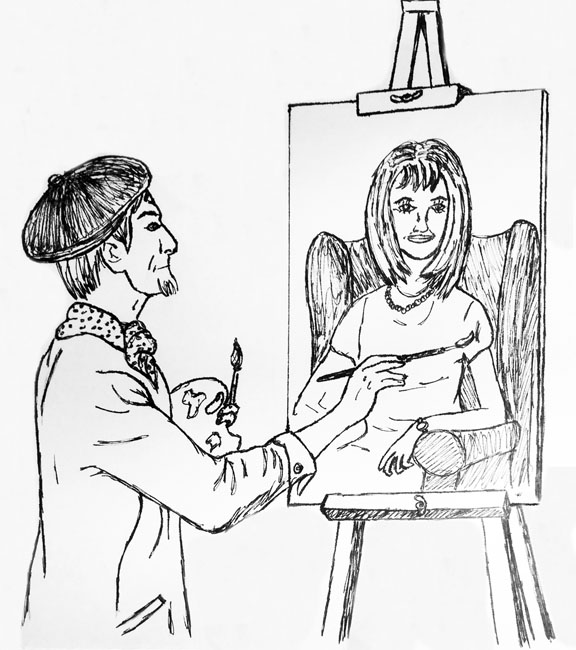
\includegraphics[width=0.55\columnwidth]{figures/exampleprompt.jpg}\\
\hline
\textbf{Response (L1)} \\
\hline
He is droning his wife pitcher. (Arabic)\\
\hline
The artist is drawing a pretty women. (Chinese) \\
\hline
The artist is painting a portrait of a lady. (English) \\
\hline
The painter is painting a woman's paint. (Spanish)\\
\hline
\end{tabular}
\end{center}
\caption{Example item and NNS responses from previous study.}
\label{fig:example-picture}
\end{figure}

The PDT consisted of 10 items (8 line drawings and 2 photographs) intended to elicit a single sentence each; an example is given in Figure~\ref{fig:example-picture}. Participants were asked to view the image and ``describe the action in either past or present tense.'' Responses were typed by the participants themselves in a computer lab with spell checking disabled.
I collected responses from 53 participants for a total of 530 sentences. There were 14 NSs (non-linguistics undergraduate and graduate students) and 39 NNSs (university students enrolled in English as a Second Language courses).

My process was to parse a NNS sentence into a dependency representation
%(section~\ref{sec:syntactic-form})
and then extract and lemmatize a semantic triple from this parse
%(section~\ref{sec:semantic-form})
to compare to a set of gold standard semantic triples similarly derived from the NS responses. As in my current research, I used the Stanford Parser for this task, trained on the Penn Treebank \citep{demarneffe:ea:06, klein:manning:03}.\footnote{\url{http://nlp.stanford.edu/software/lex-parser.shtml}} 

I manually categorized the 530 sentences in the dataset into 11 types plus one catch-all category, as shown in
Table~\ref{tab:sentence-type}. I established these types because each
one corresponds to a basic sentence structure and thus has consistent
syntactic features, leading to predictable patterns in the dependency
parses.


%\subsection{Obtaining a syntactic representation}
%\label{sec:syntactic-form}
%Because dependency parsing focuses on identifying dependency
%relations, rather than constituents or phrase structure, it clearly
%labels the subject, verb and object of a sentence, which can then map
%to a semantic form \citep{Kuebler.McDonald.Nivre-09}. In these experiments, I took a na\"ive approach in which subject, verb and
%object were considered sufficient for deciding whether or not a
%response accurately describes the visual prompt.

%
%Using the parser's options, I set the output to be Stanford typed
%dependencies, a set of labels for dependency relations. The Stanford
%parser has a variety of options for the specific
%ouput, e.g., how one wishes to treat prepositions
%\citep{defmarneffe:manning:12}.  I used only two non-default parser options ({\tt
%  CCPropagatedDependencies} and {\tt CCprocessed}\footnote{\url{http://nlp.stanford.edu/software/dependencies_manual.pdf}}) in order to:
%%
%1) omit prepositions and conjunctions from the sentence text and
%instead add the word to the dependency label between content words;
%and 2) propagate relations across conjunctions.  These decisions
%are important to consider for any semantically-informed processing of
%learner language.
%
%To see the impetus for removing prepositions, consider the learner
%example in Figure~\ref{fig:prep-dependency}, where the preposition \textit{with} is
%relatively unimportant to collecting the meaning.  Additionally,
%learners often omit, insert, or otherwise use the wrong preposition
%\citep{chodorow:et:al:07}.  The default parser would present a
%\texttt{prep} relation between \textit{played} and \textit{with},
%obscuring what the object is; with the options set as above, however,
%the dependency representation folds the preposition into the label
%(\texttt{prep\_with}), instead of keeping it in the parsed string, as
%shown in Figure~\ref{fig:prep-dependency}.
%
%\begin{figure}[htb!]
%\begin{center}
%    \begin{dependency}[arc edge,text only label,label style={above}]
%    \begin{deptext}[column sep=.5em]
%      \textit{vroot} \& The \&[1em] boy \&[1em] played \& with \& a \&[1em] ball \\
%    \end{deptext}
%    \depedge{4}{3}{nsubj}
%    \depedge[arc angle=90]{1}{4}{root}
%    \depedge{4}{7}{prep\_with}
%%    \depedge[arc angle=35,edge style={dotted}]{7}{6}{det}
%%    \depedge[edge style={dotted}]{3}{2}{det}
%    \depedge[arc angle=35]{7}{6}{det}
%    \depedge{3}{2}{det}
%  \end{dependency}
%\end{center}
%\caption{Dependency parse showing collapsed preposition dependencies.}
%\label{fig:prep-dependency}
%\end{figure}
%
%%\lk{it may be worthwhile to add the conll parse for this example so it's clear how these graphs come about}
%This is a lenient approach to prepositions, as prepositions
%are not without semantic meaning---e.g., \textit{the boy played in a
%  ball} means something quite different from the \textit{with} example.  However, this option makes it moderately easier to compare the meaning to an expected semantic form (e.g., \textit{play(boy,ball)}).
%
%As for propagating relations across conjunctions, this also simplifies the representation somewhat and makes it easier to connect verbs and their arguments, as needed for the semantic
%form used in comparisons. For a conjunction like \textit{cats and dogs}, for example, the default settings would produce \texttt{cc(cats, and)} and \texttt{conj(cats, dogs)}, but the chosen settings would collapse this into \texttt{conj\_and(cats, dogs)}, omitting the dependency that merely labels a conjunction relation between the first conjunct and the conjunction.

%Given the rule-based approach to matching \textit{verb(subject,object)} triples, many dependency relations are irrelevant for the next step of obtaining a semantic form.  For example, in this work I ignored determiner (\texttt{det}) relations between a noun and its determiner, allowing for variability in how a learner produces noun phrases. 

%\subsection{Obtaining a semantic representation}
%\label{sec:semantic-form}
%
%\subsubsection{Sentence types}

\begin{table*}[htb!]
\begin{center}
\begin{tabular}{|c|l|l|r|r|}
\hline
Type & Description & Example & NS & NNS \\
\hline
 A & Simple declarative transitive & The boy is kicking the ball. & 117 & 286 \\
 \hline
 B & Simple + preposition & The boy played with a ball. & 5 & 23 \\
 \hline
 C & Missing tensed verb & Girl driving bicycle. & 10 & 44 \\
 \hline
 D & Missing tensed verb + preposition & Boy playing with a ball. & 0 & 1 \\
 \hline
 E & Intransitive (No object) & A woman is cycling. & 2 & 21 \\
 \hline
 F1 & Passive & An apple is being cut. & 4 & 2 \\
 \hline
 F2 & Passive with agent & A bird is shot by a man. & 0 & 6 \\
 \hline
 Ax & Existential version of A or C & There is a boy kicking a ball. & 0 & 0 \\
 \hline
 Bx & Existential version of B  or D & There was a boy playing with a ball. & 0 & 0 \\
 \hline
 Ex & Existential version of E & There is a woman cycling. & 0 & 0 \\
 \hline
 F1x & Existential version of F1 & There is an apple being cut. & 0 & 1 \\
 \hline
 F2x & Existential version of F2 & There is a bird being shot by a man. & 0 & 0 \\
 \hline
 Z & All other forms & The man is trying to hunt a bird. & 2 & 6 \\
 \hline
\end{tabular}
\end{center}
\caption{Sentence type examples, with distributions of types for
  native speakers (NS) and non-native speakers (NNS)}
\label{tab:sentence-type}
\end{table*}

%\subsubsection{Rules for sentence types}

A sentence type indicates that the subject,
verb, and object can be found in a consistent place in the parse,
e.g., under a particular dependency label.
For example, for simple transitive sentences (type \textit{A} in Table~\ref{tab:sentence-type}),
the words labeled {\tt nsubj}, {\tt root}, and {\tt dobj} 
pinpoint the necessary information.
Thus, the patterns for extracting semantic information---in the form
of \textit{verb(subj,obj)} triples---reference particular Stanford
typed dependency labels, part-of-speech (POS) tags, and locations
relative to word indices (see Figure~\ref{fig:conll}).

\begin{figure}[htb!]
\begin{center}
\begin{tabular}{|C{4em}|C{5em}|C{4em}|C{4em}|C{4em}|}
\hline
\textbf{Index} & \textbf{Word} & \textbf{POS} & \textbf{Head} & \textbf{Label} \\
\hline
0 & \textit{root} & ROOT & 0 & root \\
\hline
1 & the & DET & 2 & det \\
\hline
2 & boy & NN & 4 & nsubj \\
\hline
3 & is & VBZ & 4 & aux \\
\hline
4 & kicking & VBG & 0 & root \\
\hline
5 & the & DT & 6 & det \\
\hline
6 & ball & NN & 4 & dobj \\
\hline
\hline
    \multicolumn{5}{|c|}{\begin{dependency}[arc edge,text only label,label style={above}]
    \begin{deptext}[column sep=.5em]
      ROOT \& DET \&[1em] NN \& VBZ \&[1em] VBG \& DET \&[1em] NN \\
      \textit{root} \& The \&[1em] boy \& is \&[1em] kicking \& the \&[1em] ball \\
    \end{deptext}
    \depedge[arc angle=90]{5}{3}{nsubj}
    \depedge{5}{4}{aux}
    \depedge[arc angle=92]{1}{5}{root}
    \depedge[arc angle=80]{5}{7}{dobj}
%    \depedge[arc angle=35,edge style={dotted}]{7}{6}{det}
%    \depedge[edge style={dotted}]{3}{2}{det}
    \depedge[arc angle=35]{7}{6}{det}
    \depedge{3}{2}{det}
  \end{dependency}} \\
\hline
\end{tabular}
\end{center}
%\caption{The dependency parse of an example NNS response in CoNLL\footnote{Standard dependency parse format established by the Conference on Computational Natural Language Learning (CoNLL).} format and the corresponding visual representation.}
\caption{The dependency parse of an example NNS response in a standard format (CoNLL) and the corresponding visual representation.}
\label{fig:conll}
\end{figure}

%More complicated sentences or those containing common learner errors
%(e.g., omission of the copula \textit{be}) required slightly more
%complicated extraction rules, but, since this work examined only transitive
%verbs, these still boiled down to identifying the
%sentence type and extracting the appropriate triple.
Determining the sentence type is accomplished by arranging a small set of binary decisions into a tree, as shown in Figure~\ref{fig:decision-tree}. This decision tree checks for the presence of various dependency labels. The extraction rules for the particular sentence type are then applied to obtain the semantic triple. Finally, for each NNS response, the resulting triple was checked against the gold standard list of NS triples. Ideally, each acceptable response should find a match, and unacceptable responses should not.

\begin{figure*}[htb!]
\begin{center}
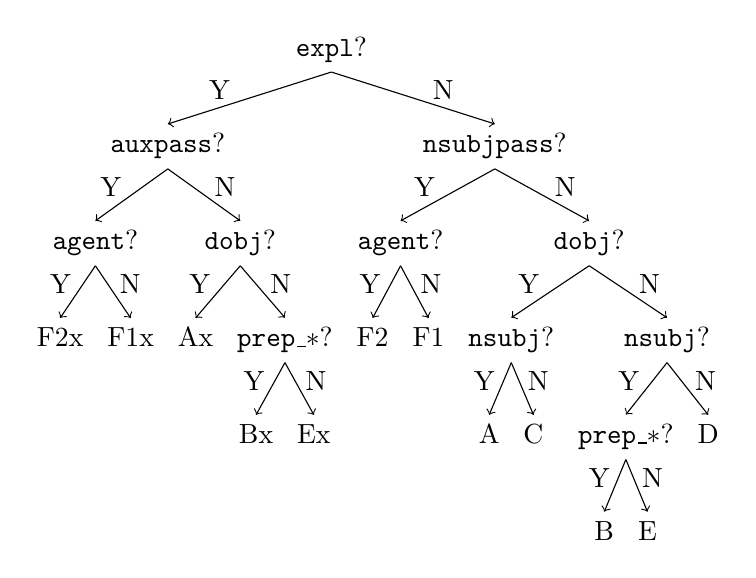
\begin{tikzpicture}
\tikzset{level distance=3.5em}
\tikzset{edge from parent/.append style={->}}
\Tree
[.{\tt expl}?
  \edge node[auto=right,pos=.6,inner sep=1pt]{Y};
  [.{\tt auxpass}? 
  	\edge node[auto=right,pos=.6,inner sep=1pt]{Y};
  	[.{\tt agent}? 
		\edge node[auto=right,pos=.6,inner sep=1pt]{Y};
		[.F2x ]
		\edge node[auto=left,pos=.6,inner sep=1pt]{N};
		[.F1x ]
	]
	\edge node[auto=left,pos=.6,inner sep=1pt]{N};
	[.{\tt dobj}? 
		\edge node[auto=right,pos=.6,inner sep=1pt]{Y};
		[.Ax ]
		\edge node[auto=left,pos=.6,inner sep=1pt]{N};
		[.{\tt prep\_}$\ast$?
			\edge node[auto=right,pos=.6,inner sep=1pt]{Y};
			[.Bx ]
			\edge node[auto=left,pos=.6,inner sep=1pt]{N};
			[.Ex ]
		]
	]
  ]
  \edge node[auto=left,pos=.6,inner sep=1pt]{N};
  [.{\tt nsubjpass}? 
  	\edge node[auto=right,pos=.6,inner sep=1pt]{Y};
  	[.{\tt agent}? 
		\edge node[auto=right,pos=.6,inner sep=1pt]{Y};
		[.F2 ]
		\edge node[auto=left,pos=.6,inner sep=1pt]{N};
		[.F1 ]
	]
	\edge node[auto=left,pos=.6,inner sep=1pt]{N};
	[.{\tt dobj}? 
		\edge node[auto=right,pos=.6,inner sep=1pt]{Y};
		[.{\tt nsubj}?
			\edge node[auto=right,pos=.6,inner sep=1pt]{Y};
			[.A ]
			\edge node[auto=left,pos=.6,inner sep=1pt]{N};
			[.C ]
		]
		\edge node[auto=left,pos=.6,inner sep=1pt]{N};
		[.{\tt nsubj}?
			\edge node[auto=right,pos=.6,inner sep=1pt]{Y};
			[.{\tt prep\_}$\ast$?
			 	\edge node[auto=right,pos=.6,inner sep=1pt]{Y};
				[.B ]
				\edge node[auto=left,pos=.6,inner sep=1pt]{N};
				[.E ]
			]
			\edge node[auto=left,pos=.6,inner sep=1pt]{N};
			[.D ]
			]
		]
	]
  ]
]
\end{tikzpicture}
\end{center}
\caption{Decision tree for determining sentence type and extracting semantic triple}
\label{fig:decision-tree}
\end{figure*}

%To illustrate, consider the process for the example in Figure~\ref{fig:F2-dependency}.  The
%sentence is passed through the parser to obtain the dependency parse shown.
%The parsed sentence then moves to the
%decision tree shown in Figure~\ref{fig:decision-tree}.
%At the top of the tree, the sentence is checked for an {\tt expl}
%(expletive) label; having none, it moves rightward to the {\tt
%  nsubjpass} (noun subject, passive) node. Because a {\tt
%  nsubjpass} label is found, the sentence moves leftward to the {\tt agent}
%node. This label is also found, and because the sentence has reached a terminal node, it is labeled as a type F2 sentence.
%
%
%With the sentence now typed as F2, specific F2 extraction
%rules are applied. The logical subject is taken from under the {\tt agent} label,
%the verb from {\tt root}, and the logical object from {\tt nsubjpass},
%to obtain \textit{shot(man,bird)}, which can be lemmatized to
%\textit{shoot(man,bird)}. 
%%Very little effort goes into this process:
%%the parser is pre-built; the decision tree is small; and the
%%extraction rules are minimal.
%
%This much is possible with relatively little effort in part due to the constraints in the
%pictures.  For figure~\ref{fig:example-picture}, for example,
%\textit{the artist}, \textit{the man in the beret}, and \textit{the
%  man} are all acceptable subjects, whereas if there were multiple men
%in the picture, \textit{the man} would not be specific enough.
%%In future work, we expect to relax such constraints on image contents
%%by including rules to handle relative clauses, adjectives and other
%%modifiers in order to distinguish between references to similar
%%elements, e.g., 
%%\textit{a man shooting a bird} vs. \textit{a man reading the
%%  newspaper}.

\subsection{Rule-based matching results}
\label{sec:rule-results}

Evaluating this work required addressing two major questions.  First,
how accurately does this approach extract semantic information from potentially
innovative sentences?
%Due to the simple structures of the sentences (section~\ref{sec:sentence-distribution}), this simple system performs moderately well.
Secondly, how many semantic forms does one need in order to capture the variability in meaning in NNS sentences? I operationalized this second question by asking how well a given set of NS semantic forms models a gold standard.
% (section~\ref{sec:eval:coverage})?

An accurate extraction was defined as one in which the extraction rules chose the desired subject, verb, and object given the sentence at hand and without regard to the PDT image. Accuracy was 92.3\% for NNS responses and 92.9\% for NS responses. I attribute the high extraction scores to the constrained nature of the task and the relatively small range of sentence types it elicits. As seen in Table~\ref{tab:sentence-type}, only three sentence types account for more than 90\% of all responses. 

Assessing the coverage of NNS forms required first manually determining which extracted triples \textit{should} be matched given a hypothetical perfect gold standard set of triples. To separate the problem of coverage from extraction, I removed any incorrectly extracted triples from the NNS set and the NS gold standard.
 
I called an appropriate NNS triple found in the gold standard set a \textbf{true positive (TP)} (i.e., a correct match), and an appropriate NNS triple \textit{not found} in the gold standard set a \textbf{false negative (FN)} (i.e., an incorrect non-match), as shown in Table~\ref{tab:contingencies}. I used standard terminology here (TP, FN), but because this was an investigation of what \emph{should be} in the gold standard, these were considered
false negatives and not false positives.  To address the question of
how many (NS) sentences are needed to obtain good coverage, \textbf{coverage} was defined as recall: \textit{TP/(TP+FN)}. I reported 23.5\% coverage for unique triple
types and 51.0\% coverage for triple tokens.

\begin{table}[htb!]
\begin{center}
\begin{tabular}{|ll||l|l|}
  \hline
  & & \multicolumn{2}{c|}{NNS}\\
  & & $+$ & $-$ \\
  \hline
  \hline
  \multirow{2}{*}{NS} & Y & TP & FP \\
  \cline{2-4}
  & N & FN & TN\\
  \hline
\end{tabular}
\end{center}
\caption{Contingency table comparing presence of NS forms (Y/N) with
  correctness ($+$/$-$) of NNS forms}
\label{tab:contingencies}
\end{table}

I defined an inappropriate NNS triple (i.e., a content error)
\textit{not found} in the gold standard set as a \textbf{true negative
  (TN)} (i.e., a correct non-match). \textbf{Accuracy} based on this
gold standard---assuming perfect extraction---is defined as
\textit{(TP+TN)/(TP+TN+FN)}.\footnote{Accuracy is typically defined as (TP+TN)/(TP+TN+FN+FP), but false positives (FPs) are cases where an incorrect NNS response was in the gold standard; by removing errors from the NS responses, I prevented this scenario (i.e., FP=0).} I reported 46.4\% accuracy for types and 58.9\% accuracy for tokens.

The immediate lesson taken from this was: given a strict matching approach, NS data alone does not make a sufficient gold standard, in that many correct NNS answers are not counted as correct. I explored expanding the set of NS triples by separating individual subjects, verbs and objects from NS triples and recombining them into the various possible combinations. However, this lead to new problems as it generates a lot of nonsensical triples. Consider, for example, \textit{do(woman,shirt)}---an incorrect triple derived from the correct NS triples, \textit{wash(woman,shirt)} and \textit{do(woman,laundry)}. Instead, my current work has attempted to improve coverage by prompting NSs to give an initial PDT response, followed by a second alternative.

A related concern was that, even when only examining cases
where the meaning is literally correct, NNSs produced a wider range of
forms to describe the prompts than NSs. For example, for a picture
showing what NSs overwhelmingly described as a \textit{raking} action,
many NNSs referred to a man \textit{cleaning} an area. Literally,
this may be true, but it does not align with a NS based gold standard. 
This behavior was expected, given that learners are encouraged
to use words they know to compensate for gaps in their vocabularies
\citep{AgustinLlach2010}. This also parallels the observation in SLA research that while second language learners may attain native-like grammar, their ability to use
pragmatically native-like language is often much lower
\citep{BardoviDornyei1998}. \lk{Work a D Stringer citation in here?}
These findings highlighted the need for a more flexible approach.
%that considers how native-like a sentence is as well as how appropriate its meaning is.

Moreover, evaluating this strict matching approach required an annotator to decide whether a given response is correct or incorrect. Partial matching is not allowed; this is an inherent weakness of the approach, because while a complete triple gives some indication of the meaning of the sentence, any single element of the triple taken alone does not provide enough context to indicate meaning. This inflexibility means that using this approach would effectively require the manual curation of a robust gold standard set of acceptable responses, which is counter to my goal of producing an approach that can be expanded to new PDT items simply by crowdsourcing a gold standard from NSs.

%\begin{table}[htb!]
%\begin{center}
%\begin{tabular}{|c|c|}
%\hline
%Triple & Example sentence \\
%\hline
%\hline
%shoot(man, bird) & A man just shot a bird. \\
% \hline
%shoot(man, fowl) & The man shoots the fowl. \\
% \hline
%shoot(man, duck) & A man just shot a duck. \\
% \hline
%shoot(hunter, bird) & The hunter has shot a bird. \\
% \hline
%shoot(he, bird) & He shot the bird down! \\
% \hline
% \end{tabular}
%\end{center}
%\caption{The NS gold standard for Item 10.}
%\label{tab:item10GS}
%\end{table}

I followed up this work with a modification of this strict matching approach that included  language models and spell checking tools to attempt to identify and fix misspellings that lead to downstream problems \citep{king:dickinson:14}. I omit this discussion because it is not applicable to the current work; I now take a simpler approach --- respondents use spell checking during the task. This is because in most contexts where my system would be used, like a language tutoring application or game, spelling instruction is not the objective, and a built-in spell checker would likely be available. Moreover, omitting this step removes a layer of analysis---and importantly, a potential source of errors---and allows the research to focus more directly on meaning.

%%%% END material from Qual Paper (BEA 2013) %%%%


%%%% BEGIN material from BEA 2016 %%%%
\section{Recent work: Generalized, similarity-based approaches}

%%%% 2020/05/21. Resume here. %%%% 

In subsequent work \citep{king:dickinson:16}, I began looking for a ``sweet spot'' of
semantic analysis \citep[cf.][]{bailey:meurers:08} for image-based learner productions. I applied new methods to the same dataset, and the current dissertation research applies a refined version of these methods to the new dataset discussed in Chapters~\ref{chap:data} and~\ref{chap:annotation}.
In particular, using available NLP tools, I moved away from specific correct semantic representations and an exact definition of correctness, to more abstract representations
and more gradable notions of correctness (section~\ref{sec:ranking}). This obviates the need for a rule-based extraction of sentence elements, which must be customized for a limited range of expected sentence types. It also allows for graded scoring of results, meaning that a response is not outright rejected because only one element of a triple is not found. On the other hand, it means that the system does not provide a discrete ``acceptable'' or ``not acceptable'' decision, which means that downstream tasks like assessment, providing feedback or effecting game outcomes would require more careful consideration of what to do with the system output.

I should note, in this context, that I am discussing semantic
analysis given a gold standard set of NS sentences.  Image processing
tasks often rely on breaking images into semantic primitives
\citep[see, e.g.,][and references therein]{ortiz:wolff:lapata:15}, but
for NNS data, I want to ensure that I can account not just for
correct semantics (the \emph{what} of a picture), but natural
expressions of the semantics (the \emph{how} of expressing the
content).  In other words, the goal is to reason about meaning based on
specific linguistic forms.

A second issue regarding content analysis, beyond correctness, stems
from using an incomplete GS. The productive nature of language means that a sentence can be expressed in countless ways, and thus a GS can never really be ``complete''. Examining the degree of this variability both for NSs and NNSs is necessary to determine whether a crowd-sourced gold standard can account for a sizable portion of test responses. Analyzing variability can also help determine the most effective parameters for an NLP system for image based responses. Additionally, it can offer insights into theoretical research on variability in learner language (cf. \citet{ellis1987variability}, \citet{kanno1998consistency}).

%That is, different types of image content might require
%different mechanisms for processing.  Additionally, knowing how
%different pictures elicit different kinds of content can provide
%feedback on appropriate types of new data to collect.
%We approach this issue by clustering responses in various ways
%(section~\ref{sec:clustering}) and seeing how the clusters connect to
%system parameters.
%
%For both the experiments involving the accuracy of different system
%parameters (section~\ref{sec:ranking}) and the clustering of different
%responses (section~\ref{sec:clustering}), we present results within
%those sections that show the promise of moving to abstract representations, but in
%different ways for different kinds of data.
%
%We build directly from \citet{king:dickinson:13,king:dickinson:14},
%where the method to obtain a semantic form from a NNS production is:
%1) obtain a syntactic dependency representation from the off-the-shelf
%Stanford Parser \citep{demarneffe:ea:06, klein:manning:03}, and 2)
%obtain a semantic form from the parse, via a small set of hand-written
%rules.  It is this method we attempt to generalize
%(section~\ref{sec:ranking}).

%\section{Data Collection}
%\label{sec:data}
%
%Because our approach requires both NS and NNS responses and
%necessitates constraining both the form and content of responses, we
%previously assembled a small corpus of NS and NNS responses to a PDT
%\citep{king:dickinson:13}.  Research in SLA often relies on the
%ability of task design to induce particular linguistic behavior
%\citep{skehan1998assessing}, and the PDT should induce context-focused
%communicative behavior.  Moreover, the use of the PDT as a reliable
%language research tool is well-established in areas of study ranging
%from SLA to Alzheimer's disease \citep{ellis2000task,
%forbes2005detecting}.

%
%The PDT consists of 10 items (8 line drawings and 2 photographs\footnote{We have not observed substantial differences between responses for the drawings and the photographs.}) intended to elicit a single sentence
%each; an example is given in Figure~\ref{fig:example-picture}. Participants
%were asked to view the image and describe the action in past or present tense.
%The data consist of responses from 53 informants (14 NSs, 39 NNSs),
%for a total of 530 sentences, with the NNSs being intermediate and
%upper-level adult English learners in an intensive English as a Second
%Language program.  The distribution of first languages (L1s) is: 14
%English, 16 Arabic, 7 Chinese, 2 Japanese, 4 Korean, 1 Kurdish, 1
%Polish, 2 Portuguese, and 6 Spanish.
%
%Responses were typed by the participants themselves, with spell checking disabled in some cases.  Even among the NNSs that used spell checking, a number of spelling errors resulted in real words. To address this, we use a spelling correction tool to obtain candidate spellings for each word, prune the candidates using word lists from the NS responses, recombine candidate spellings into candidate sentences, and evaluate these with a trigram language model (LM) to select the most likely intended response \citep{king:dickinson:14}.
%
%Once the responses had been collected, the NNS responses were
%annotated for correctness, with respect to the content of the picture.
%The lead author marked spelling and meaning errors which prevent a
%complete mapping to correct information
%\citep[see][]{king:dickinson:13}.  On the one hand, minor misspellings
%are counted as incorrect (e.g., \textit{The artiest is drawing a
%\textbf{portret}}), while, on the other hand, the annotation does
%not require distinguishing between between spelling and meaning
%errors.  In the future, we plan on fine-tuning the annotation
%criteria.
\bigskip
START HERE 2021/01/15
\bigskip

\subsection{Generalizing the Methods}
\label{sec:ranking}

The previous work assumed that the assessment of NNS responses
involves determining whether a gold standard set contains the same
semantic triple that the NNS produced, i.e., whether a \textit{triple}
is \textit{covered} or \textit{non-covered}.  In such a situation the
gold standard need only be comprised of \textit{types} (not \textit{tokens}) of semantic triples. But the gold standard is comprised of the small set of NS responses---here, only 14---and is thus incomplete. This means that exact matching is going to miss many cases,
and indeed as discussed in Section~\ref{sec:rule-results}, coverage was only at 51\%. Even with a much larger sample of NS responses, a gold standard will always be incomplete. Additionally, relying on matching of triples limits the utility of the method to specific semantic requirements, namely transitive sentences.  By changing to ``bags of dependencies'' and tallying the counts of dependencies in the NS responses comprising the gold standard, I moved into a gradable, or ranking, approach to NNS responses.

My goal is to emphasize the degree to which a response conveys the same
meaning as the GS, necessitating an approach which can automatically
determine the importance of a piece of information in the GS.  In Section~\ref{sec:representation}, I detail how I represented the information
 and in Section~\ref{sec:scoring}, I discuss comparing NNS
information to GS information, which allowed me
to rank responses from least to most similar to the GS.\footnote{Although rankings often go from highest to lowest, I prioritize identifying problematic cases, so I rank accordingly.}
%I also discuss the handling of various other system parameters (section~\ref{sec:parameters}).

This work used the same 10 item PDT dataset described in section~\ref{sec:first-approaches}. Another example is shown in Figure~\ref{fig:example-picture2}.

\begin{figure}
\begin{center}
\begin{tabular}{|c|}
\hline
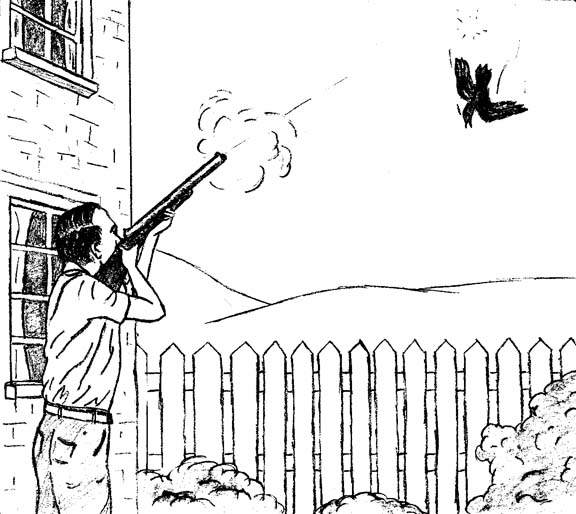
\includegraphics[width=0.7\columnwidth]{figures/exampleprompt2.jpg}\\
\hline
\textbf{Response (L1)} \\
\hline
The man killing the beard. (Arabic)\\
\hline
A man is shutting a bird. (Chinese) \\
\hline
A man is shooting a bird. (English) \\
\hline
The man shouted the bird. (Spanish)\\
\hline
\end{tabular}
\end{center}
\caption{Example item and responses}
\label{fig:example-picture2}
\end{figure}

\subsection{Representation}
\label{sec:representation}

To overcome the limitations of an incomplete GS, I represented each
response as a list of \textit{terms} taken from the dependency parse
\citep{demarneffe:ea:06}, the terms referring to
%being either 
individual dependencies (i.e., relations between words).
%or individual words. 
This eliminates the complications of extracting semantic triples from
dependency parses, which only handled a very restricted set of
sentence patterns and resulted in errors in 7--8\% of cases
\citep{king:dickinson:13}. Operating directly on individual
%words or
dependencies from the overall tree also means the system can allow for
``partial credit''; it distributes the matching over smaller,
overlapping pieces of information rather than a single, highly
specific triple.

Specifically, representations took one of five forms.  I first
tokenized and lemmatized a response to a list of dependencies that
represents the response.
The five term representations are then variations on dependencies. The
full form concatenates the label, head and dependent, as in
\texttt{subj\#boy\#kick}. I call this \textbf{ldh} (label, dependent,
head). The remaining four forms abstract over either the label, head
and/or dependent, as in \texttt{X\#boy\#kick}. I refer to these forms
as \textbf{xdh}, \textbf{lxh}, \textbf{ldx}, and \textbf{xdx}. I tested the system performance using each of these term representations separately.

The \param{xdx} model is on a par with treating the sentence as a ``bag
of words'' (or more accurately, a bag of lemmas), except that some function words not receiving parses (e.g., prepositions) are not included (see section~\ref{sec:syntactic-form}).

\subsection{Scoring Responses}
\label{sec:scoring}

Taking the term representations from the previous section, my next
step was to combine them in a way which ranks responses from least to
most appropriate.  I scored the responses with one of four approaches, each
using one of two methods to \textbf{weight} response terms combined
with one of two methods to \textbf{compare} the weighted NNS terms
with the GS.

For weighting, I used either a simple frequency measure
or one based on term frequency-inverse document frequency (\textbf{tf-idf})
\citep[][ch. 6]{manning-et-al:08}.  I used tf-idf as a measure of
a term's importance with the hope that it could reduce the impact
of semantically unimportant terms---e.g., determiners like
\textit{the}, frequent in the GS, but unimportant for evaluating the
semantic contents of NNS responses---and to upweight terms which may
be salient but infrequent, e.g., only used in a handful of GS
sentences. For example, for an item depicting a man shooting a bird
(see Table~\ref{tab:i10responses-avgprec} and Figure~\ref{fig:example-picture}), of 14 GS responses, 12
described the subject as \textit{man}, one as \textit{he} and one as
\textit{hunter}. Since \textit{hunter} is relatively infrequent in English, even
one instance in the GS should get upweighted via tf-idf, and indeed it
that was the effect. 
This is valuable, as numerous NNS responses used \textit{hunter}.

Calculating tf-idf relies on both \emph{term frequency} ($tf$) and
\emph{inverse document frequency} ($idf$).  Term frequency is simply
the raw count of a term, and for tf-idf of terms in the GS, I take
this as the frequency within the GS.  Inverse document frequency is
derived from some reference corpus, and it is based on the notion that
appearing in more documents makes a term less informative with respect
to distinguishing between documents.  The formula is in
(\ref{ex:tfidf}) for a term $t$, where $N$ is the number of documents
in the reference corpus, and $df_{t}$ is the number of documents
featuring the term ($idf_{t} = \log \frac{N}{df_{t}}$).  A term
appearing in fewer documents will thus obtain a higher $idf$ weight,
and this should readjust frequencies based on semantic importance.

\begin{exe}
\ex\label{ex:tfidf} $tfidf(t) = tf_{GS} \log \frac{N}{df_{t}}$
%, where $df_t = |\{d\in D, t \in d\}|$
\end{exe}

After this counting or weighting, the scores are then either
\textbf{averaged} to yield a response score, or NNS term
weights and GS term weights are treated as vectors and the response
score is the \textbf{cosine distance} between them.  This
yields:

%%former approach names: b = FA; m = IC (TC); c = FC; a = IA (TA)
\paragraph{Frequency Average (FA).} 
%This approach serves as our baseline. 
Within the GS, the frequency of each term is calculated. Each term in
the NNS response is then given a score equal to its frequency in the
GS; terms missing from the GS are scored zero. The response score is
the average of the term scores, with higher scores closer to the GS.

\paragraph{Tf-idf Average (TA).} This involves the exact same
averaging as with model FA, but now the terms in the GS are assigned
tf-idf weights before averaging.

\paragraph{Frequency Cosine (FC).} The frequency of each term is
calculated within the GS and (separately) within the NNS response. 
The term scores are then treated as vectors, and the response score is
the cosine distance between them, with lower scores being closer to
the GS.

\paragraph{Tf-idf Cosine (TC).} This involves the exact same
distance comparison as with model FC, but now the terms of both the GS
and NNS responses are assigned tf-idf weights before comparison.

The two cosine approaches are effectively primitive versions of sentence encoders like the currently popular BERT \citep{BertDevlin2018} and Universal Sentence Encoder \citep{UniversalSentenceEncoder}. Sentence encoders are a form of language model that learns mathematical representations of words by observing them in context, accounting for things like average distance from a given word type to another given word type. Sentence encodings are thus vectors representing these word values for a full sentence. These approaches result in very high dimensional spaces---imagine a sentence representation that consists of a vector for each word in the sentence, where each vector is a list of average distances from that word type to \textit{every other word type in the language}. Thus sentence encoders typically rely on methods of dimensionality reduction to compress these representations into vectors of manageable length.
I say my cosine approaches constitute ``primitive'' encoders because they omit this step. In the case of my PDT constrained corpus, the number of word types (and in turn dependency types) observed for a given item remains small enough that the raw vectors representing dependencies' tf-idf scores can still be processed easily with a laptop computer. Not only does this simplify the process, it means that the process remains transparent. There are no opaque machine learning processes that derive compressed representations, and each sentence vector could be examined value by value, where each number represents a real dependency. This is important because it leaves the door open for meaningful feedback on each response. For example, one could identify the most salient dependencies in the GS of a given item and somehow present those to a user who gives a low scoring response in order to suggest a more appropriate response. That is to say, a full encoder could determine how similar a response is to a GS, but it could not tell us \textit{why} it made its determination.

\subsection{System Parameters}
\label{sec:parameters}

In addition to the four approaches, the five term representations and
two sets of parameters, listed below, were varied, resulting in a total of
60 settings for processing responses (see also
Table~\ref{tab:dist-ranked-parameters}). 

\paragraph{Term form.} As discussed in
section~\ref{sec:representation}, the terms can take one of five
representations: \param{ldh}, \param{xdh}, \param{lxh}, \param{ldx},
or \param{xdx}.

\paragraph{Scoring approach.} As discussed in
section~\ref{sec:scoring}, the NNS responses can be
compared with the GS via models \param{FA}, \param{TA}, \param{FC}, or \param{TC}.

\paragraph{Reference corpus.} The reference corpus for deriving tf-idf
scores can be either the Brown Corpus \citep{kucera:francis:67} or the
Wall Street Journal (WSJ) Corpus \citep{marcus-et-al:93}. These are
abbreviated as \param{B} and \param{W} in the results
below; \param{na} indicates the lack of a reference corpus, as this is
only relevant to approaches \param{TA} and
\param{TC}. The corpora are divided into as many documents as
originally distributed (\param{W}: 1640, \param{B}: 499). The WSJ is
larger, but Brown has the benefit of containing more balance in its
genres (vs. newstext only). Considering the narrative nature of PDT
responses, a reference corpus of narrative texts would be ideal, but
I chose manually parsed reference corpora as they are more reliable
than automatically parsed data.

\paragraph{NNS source.} Each response has an original version
(\param{NNSO}) and the output of a language model spelling corrector
(\param{NNSLM}). (The current dissertation relies on a corpus for which participants used spell checking at the time of the task, so this offline spelling correction is no longer applicable. In short, it used a spelling tool to find candidate spellings for each word in a NNS sentence, pruned the lists of candidate words by comparing against words in NS responses, formed new candidate sentences by combining candidate words, and finally chose the most likely sentence by rating each candidate with a trigram word model. I omit the exact details here for brevity, but more can be found in \cite{king:dickinson:14}).

\subsection{Results}

\subsubsection{Evaluation metrics}
\label{sec:metrics}

I ran 60 response experiments, each with different system settings
(section~\ref{sec:parameters}). Within each experiment, I ranked the 39
scored NNS responses from least to most similar to the GS.

For assessing these settings themselves, I relied on the past annotation,
which counted unacceptable responses as errors (see
section~\ref{sec:eval:extraction}).  As the
lowest rank indicates the greatest distance from the GS, a good system
setting should ideally position the unacceptable responses among those
with the lowest rankings. Thus, I assigned each error-containing
response a score equal to its rank, or, if necessary, the average rank
of responses sharing the same score.

In Table~\ref{tab:i10responses-avgprec}, an excerpt of sentence
responses is shown for one item, ranked from lowest to highest.  To
take one example, the third-ranked sentence, \textit{the man is hurting duck}, has a score of 0.996, and it is annotated as an error (1 in
the \textit{E} column).  Thus, the evaluation metric adds a score of 3
to the overall sum.  The sentence ranked 18, by contrast, is not an
error, and so nothing is added.  In the case of the top rank, two
responses with errors are tied, covering rank 1 and 2, so each adds a score of 1.5.

\begin{table}[htb!]
\begin{center}
\setlength{\tabcolsep}{0.3em}
\begin{tabular}{|r|c|l|r|r|}
\hline
\textit{R} & \textit{S} & Sentence & \textit{E} & \textit{V}\\
\hline
\hline
\multirow{2}{*}{1} & 1.000 & she is hurting. & 1 & 1.5 \\
& 1.000 & man mull bird & 1 & 1.5 \\
\hline
3 & 0.996 & the man is hurting duck. & 1 & 3.0 \\
4 & 0.990 & he is hurting the bird. & 1 & 3.0 \\
\hline
11 & 0.865 & the man is trying to hurt a bird & 1 & 11.0 \\
12 & 0.856 & a man hunted a bird. & 0 & 0.0 \\
\hline
17 & 0.775 & the bird not shot dead.  & 1 & 17.0 \\
18 & 0.706 & he shot at the bird & 0 & 0.0 \\
19 & 0.669 & a bird is shot by a un & 1 & 19.0 \\
20 & 0.646 & the old man shooting the birds & 0 & 0.0 \\
\hline
37 & 0.086 & the old man shot a bird. & 0 & 0.0 \\
38 & 0.084 & a old man shot a bird. & 0 & 0.0 \\
39 & 0.058 & a man shot a bird & 0 & 0.0 \\
\hline
\hline
\multicolumn{3}{|c|}{Total (Raw)} & 17 & 169 \\
\hline
\multicolumn{3}{|c|}{Average Precision} & \multicolumn{2}{c|}{0.75084} \\
\hline
\end{tabular}
\caption{Rankings for Item 10 from the best system setting (tf-idf cosine scoring, Brown Corpus for tf-idf reference, the language model spelling corrected NNS sentence, and the full label, dependent and head representation; TC\_B\_NNSLM\_ldh) based on average precision scores. \textit{R}: rank; \textit{S}: sentence score; \textit{E}: error; \textit{V}: rank value. Note that not all responses are shown. }
\label{tab:i10responses-avgprec}
\end{center}
\end{table}

The sum of these scores is taken as the \textbf{Raw} metric for that
experimental setting. In many cases, one version of a response
(\param{NNSO} or \param{NNSLM}) contains an error, but the other
version does not. Thus, for example, an \param{NNSO} experiment may
result in a higher error count than the \param{NNSLM} equivalent, and
in turn a higher Raw score.
In this sense, Raw scores emphasize error reduction and incorporate
item difficulty.

However, it is possible that the \param{NNSO} experiment, even with
its higher error count and Raw score, does a better job ranking the
responses in a way that separates good and erroneous ones. To account
for this, I also used \textbf{(mean) average precision ((M)AP)}
\citep[][ch. 8]{manning-et-al:08}, which emphasizes discriminatory
power.

For average precision (AP), one calculates the precision of error
detection at every point in the ranking, lowest to highest.  In
Table~\ref{tab:i10responses-avgprec}, for example, the precision for
the first cut-off (1.000) is 1.0, as two responses have been
identified, and both are errors ($\frac{2}{2}$). At the 11th- and
12-ranked response, precision is 1.0 ($\frac{11}{11}$) and 0.917
(=$\frac{11}{12}$), respectively, precision dropping when the item is
not an error.
AP averages over the precisions for all $m$ responses ($m=39$ for our
NNS data), as shown in (\ref{ex:ap}), with each response notated as
$R_k$.  Averaging over all 10 items results in the Mean AP (MAP).

\begin{exe}
\ex\label{ex:ap} $AP(item) = \frac{1}{m} \sum\limits_{k=1}^m
Precision(R_k)$
\end{exe}

As mentioned, the Raw metric emphasizes error reduction, as it
reflects not just performance on identifying errors, but also the
effect of the overall number of errors.
%In this way, it may be useful
%for predicting future system performance, an issue we explore in the
%evaluation of clustering items (section~\ref{sec:clusteringresults}).
MAP, on the other hand, emphasizes finding the optimal separation
between errors and non-errors and is thus more of the focus in the
evaluation of the best system parameters next.

\subsubsection{Best system parameters} 

To start the search for the best system parameters, it may help to
continue with the example in
Table~\ref{tab:i10responses-avgprec}. The best setting, as determined by the
MAP metric, uses the tf-idf cosine (\param{TC}) approach with the Brown Corpus (\param{B}),
the spelling corrected response (\param{NNSLM}), and the full form of
the dependencies (\param{ldh}). It ranks highest because errors are
well separated from non-errors; the highest ranked of 17 total errors
is at rank 19.  Digging a bit deeper, one can see in this example how
the verb \textit{shoot} is common in all the highest-ranked cases shown
(\#37--39), but absent from all the lowest, showing both the effect of
the GS (as all NSs used \textit{shoot} to describe the action) and the
potential importance of even simple representations like lemmas.  In
this case, the \param{ldh} representation is best, likely because the
word \textit{shoot} is not only important by itself, but also in terms
of which words it relates to, and how it relates (e.g.,
\texttt{dobj\#bird\#shoot}).

\begin{table*}
\begin{center}
\begin{tabular}{|l|r||l|r||l|r||l|r|}
\hline
\multicolumn{2}{|c||}{Approach} & \multicolumn{2}{|c||}{Term Form} & \multicolumn{2}{|c||}{Ref. Corpus (TA/TC)} & \multicolumn{2}{|c|}{NNS Source} \\
\hline
\hline
0.51577 & TC & xdh & 0.51810 & Brown & 0.51534 & NNSLM & 0.51937 \\
\hline
0.50780 & FC & ldh & 0.51677 & WSJ & 0.50798 & NNSO & 0.49699 \\
\hline
0.50755 & TA & lxh & 0.51350 & & & & \\
\hline
0.49464 & FA & xdx & 0.49901 & & & & \\
\hline
& 	& ldx & 0.49352 &  &  &  & \\
\hline
\end{tabular}
\caption{Approaches and parameters ranked by mean average precision for all 10 PDT items.}
\label{tab:dist-ranked-parameters}
\end{center}
\end{table*}

Table~\ref{tab:all-dist-ranked-settings} shows the five best and five
worst system settings averaged across all 10 PDT items, as ranked by
MAP. Among the trends that pop out is a favoritism
towards \param{NNSLM} models (i.e., spelling correction). This is due
to the fact that higher numbers of errors inflate the MAP scores, and
somewhat counterintuitively, the spelling correction module introduces
more errors than it corrects, meaning there are more errors present
overall in the \param{NNSLM} responses than in the \param{NNSO}
responses.\footnote{Note that among the remaining parameter classes,
variation does not effect the number of errors.}

Another feature among the best settings is the inclusion of heads in the dependency representations. In fact, the top 17 ranked settings all include heads (\param{lxh}, \param{xdh}, \param{ldh}); \param{xdx} first enters the rankings at 18, and \param{xdx} and \param{ldx} are common among the worst performers. This is likely due to the salience of the verbs in these transitive sentences; they constitute the heads of the subjects and objects, in relatively short sentences with few dependencies.
Furthermore, the tf-idf weighted models dominate the rankings, especially \param{TC}. It is also clear that for my data tf-idf works best with the Brown Corpus (\param{B}).

\begin{table}[htb!]
\begin{center}
\begin{tabular}{|r|l|c|}
\hline
Rank & MAP & Settings \\
\hline
\hline
1 & 0.5534 & TC\_B\_NNSLM\_lxh \\
\hline
2 & 0.5445 & TA\_B\_NNSLM\_lxh \\
\hline
3 & 0.5435 & TC\_W\_NNSLM\_lxh \\
\hline
4 & 0.5422 & TC\_B\_NNSLM\_xdh \\
\hline
5 & 0.5368 & TC\_B\_NNSLM\_ldh \\
\hline
\hline
56 & 0.4816 & TA\_B\_NNSO\_xdx \\
\hline
57 & 0.4796 & FA\_na\_NNSLM\_ldx \\
\hline
58 & 0.4769 & FC\_na\_NNSO\_lxh \\
\hline
59 & 0.4721 & TA\_W\_NNSO\_xdx \\
\hline
60 & 0.4530 & FA\_na\_NNSO\_lxh \\
\hline
\end{tabular}
\caption{Based on Mean Average Precision, the five best and five worst settings across all 10 PDT items.}
\label{tab:all-dist-ranked-settings}
\end{center}
\end{table}

I also summarize the rankings for the individual parameter classes,
presented in Table~\ref{tab:dist-ranked-parameters}, confirming the
trends in Table~\ref{tab:all-dist-ranked-settings}. For a given
parameter, e.g., \param{ldh}, I averaged the experiment scores from
all settings including \param{ldh} across all 10 items. Notably, \param{TC} outperforms the other models, with \param{FC} and \param{TA} close behind (and nearly tied). Performance falls for the simplest model, \param{FA}, which was in fact intended as a baseline. With \param{TC}$>$\param{FC} and \param{TA}$>$\param{FA}, tf-idf weighting seems preferable to basic frequencies.

Again, the importance of including heads in dependencies is apparent here; the three dependency representations containing heads constitute the top three, with a sizable drop in performance for the remaining two forms (\param{xdx} and \param{ldx}). Moreover, given the content and narrative style of the PDT responses, it is unsurprising that the Brown Corpus serves as a better reference corpus than the WSJ Corpus for tf-idf. Finally, the \param{NNSLM} source significantly outperforms the \param{NNSO} source.

Despite the strength of these overall trends, variability
does exist among the best settings for different items, a point obscured
in the averages.  In Tables~\ref{tab:i01-dist-ranked-settings} and
\ref{tab:i05-dist-ranked-settings}, I present the best and worst
ranked settings for two of the least similar items, 1 and 5.
Their dissimilarity can be seen at a glance, simply from the range of
the AP scores (0.05--0.31 for item 1 vs. 0.52--0.81 for item 5), which
in itself reflects a differing number of erroneous responses (2 [\param{NNSO}]
or 6 [\param{NNSLM}] for item 1 vs. 23 or 24 for item 5).

For item 1, a drawing of a boy kicking a ball, there is considerable
variability in the best scoring approach just within the top five settings:
all four approaches (TA, TC, FA, FC) are in the top five.  Contrary to the overall
trends, I also found the \param{ldx} form---without any head
information---in the two best settings.  Note also that, even though
tf-idf weighting (\param{TA}/\param{TC}) is usually among the best settings, it is
occurs among the worst settings, too.

For item 5 in Table~\ref{tab:i05-dist-ranked-settings}, a drawing of a
man raking leaves, the most noticeable difference is that
of \param{xdx} being among three of the top five settings.
I believe that part of the reason for
the higher performance of \param{xdx} (cf. lemmas), is that for this
item, all the NSs use the verb \textit{rake}, while none of the NNSs use this word.  For item 1 (the boy kicking a ball), there is lexical variation
for both NSs and NNSs.

\begin{table}[htb!]
\begin{center}
\begin{tabular}{|r|c|c|}
\hline
Rank & AP & Settings \\
\hline
\hline
1 & 0.30997 & TC\_B\_NNSLM\_ldx \\
\hline
2 & 0.30466 & TA\_B\_NNSLM\_ldx \\
\hline
3 & 0.30015 & TA\_B\_NNSLM\_xdh \\
\hline
4 & 0.29704 & FC\_na\_NNSLM\_xdh \\
\hline
5 & 0.29650 & FA\_na\_NNSLM\_ldh \\
\hline
\hline
56 & 0.06474 & TC\_B\_NNSO\_ldx \\
\hline
57 & 0.06174 & TC\_W\_NNSO\_ldx \\
\hline
58 & 0.06102 & TA\_W\_NNSO\_lxh \\
\hline
59 & 0.05603 & TA\_W\_NNSO\_xdx \\
\hline
60 & 0.05094 & TA\_W\_NNSO\_ldx \\
\hline
\end{tabular}
\caption{Based on Average Precision, the five best and five worst settings for item 1.}
\label{tab:i01-dist-ranked-settings}
\end{center}
\end{table}

\begin{table}[htb!]
\begin{center}
\begin{tabular}{|r|c|c|}
\hline
Rank & AP & Settings \\
\hline
\hline
1 & 0.80965 & FA\_na\_NNSLM\_xdx \\
\hline
2 & 0.80720 & TA\_B\_NNSLM\_lxh \\
\hline
3 & 0.80473 & TC\_B\_NNSLM\_lxh \\
\hline
4 & 0.79438 & TC\_B\_NNSLM\_xdx \\
\hline
5 & 0.78108 & TC\_W\_NNSLM\_xdx \\
\hline
\hline 
56 & 0.56495 & FC\_na\_NNSO\_xdh \\
\hline
57 & 0.56414 & TC\_B\_NNSO\_lxh \\
\hline
58 & 0.55890 & TC\_W\_NNSO\_lxh \\
\hline
59 & 0.54506 & FC\_na\_NNSO\_lxh \\
\hline
60 & 0.52013 & FA\_na\_NNSO\_lxh \\
\hline
\end{tabular}
\caption{Based on Average Precision, the five best and five worst settings for item 5.}
%%LK: fixed 4/6 pm.
\label{tab:i05-dist-ranked-settings}
\end{center}
\end{table}

These types of differences---for these items and others---lead me to explore the clustering of item patterns, in order to
leverage these differences and automatically choose the optimal
settings for new items; we turn to this next.

%\section{Clustering}
%\label{sec:clustering}
%
%Given the variability of NS and NNS responses, and the possible
%correlation with different system parameters, we have begun exploring
%connections by clustering the different items.  The clustering uses,
%for one set, \emph{response features}, i.e., features observable from
%the responses, and, separately, \emph{performance features}, i.e., the
%performance of different system settings on the responses.
%
%Although the work is very exploratory, our goal is to get a handle on
%learner variability for different items and explore correlations
%between response and performance clusters.
%
%\subsection{Response Clustering}
%
%We cluster the 10 PDT items using simple features taken from the
%responses themselves. Specifically, we use various combinations of
%type counts, token counts, and type-to-token ratios for each term form
%(\param{ldh}, \param{xdh}, \param{lxh}, \param{ldx}, \param{xdx}),
%taken from each response source (GS, \param{NNSO}, \param{NNSLM}).
%
%\subsection{Performance Clustering}
%
%From the system output, we cluster items using per-item Raw 
%scores for various settings. That is, for each of the 10 items, we
%calculate an average error score for each approach
%(\param{FA}, \param{TA}, \param{FC}, \param{TC}), each term form
%(\param{ldh}, \param{xdh}, \param{lxh}, \param{ldx}, \param{xdx}),
%each reference corpus (\param{B}, \param{W}), and each
%response source (\param{NNSO}, \param{NNSLM}). 
%As mentioned in section~\ref{sec:metrics}, Raw scores should account for the number of
%errors produced by NNSs for each item, which should 
%correlate with future system performance.
%
%\subsection{Results}
%\label{sec:clusteringresults}
%
%Although there is noise in some experiments, some patterns do seem to
%emerge in many of the clusterings; we present some of the most common
%patterns here.
%
%Figure~\ref{fig:response-clusters} shows a clustering based on
%response features that shares some characteristics with
%Figure~\ref{fig:parameter-clusters}, a clustering based on performance
%features. (Note that clustering heights are not to scale.)  In both
%examples, items 5 and 9 form a cluster attaching to the root. These
%are described in the GS as \textit{A man is raking leaves} and
%\textit{Two boys are rowing a boat}. These were also the two most
%difficult items for NNSs. While other items involved common verbs like
%\textit{kick}, \textit{paint} and \textit{cut}, the actions depicted
%in these items were more specific and required words outside the
%vocabulary of many participants. For example, while all 14 NSs used
%either \textit{row} or \textit{paddle}, only five of 39 NNSs used
%these verbs; the rest used verbs like \textit{boat}, \textit{sail},
%\textit{sit}, \textit{play} or \textit{ride}.
%
%\begin{figure}
%\begin{center}
%\begin{tikzpicture}[sloped]
%\node (5) at (-7.5,0) {5};
%\node (9) at (-6.9,0) {9};
%\node (1) at (-6.2,0) {1};
%\node (4) at (-5.5,0) {4};
%\node (6) at (-4.7,0) {6};
%\node (2) at (-4.0,0) {2};
%\node (8) at (-3.2,0) {8};
%\node (10) at (-2.6,0) {10};
%\node (3) at (-1.8,0) {3};
%\node (7) at (-1.1,0) {7};
%\node (59) at (-7.2,0.7) {};
%\node (14) at (-5.9,0.7) {};
%\node (28) at (-3.5,0.7) {};
%\node (37) at (-1.5,0.7) {};
%\node (1037) at (-2.3,1) {};
%\node (281037) at (-2.9,1.3) {};
%\node (6281037) at (-3.6,1.7) {};
%\node (146281037) at (-4.9,2.1) {};
%\node (59146281037) at (-6.4,2.5) {};
%\draw  (5)  |- (59.center);
%\draw  (9)  |- (59.center);
%\draw  (1)  |- (14.center);
%\draw  (4)  |- (14.center);
%\draw  (2)  |- (28.center);
%\draw  (8)  |- (28.center);
%\draw  (3)  |- (37.center);
%\draw  (7)  |- (37.center);
%\draw (10) |- (1037.center);
%\draw (37) |- (1037.center);
%\draw (1037) |- (281037.center);
%\draw (28) |- (281037.center);
%\draw (6) |- (6281037.center);
%\draw (281037) |- (6281037.center);
%\draw (14) |- (146281037.center);
%\draw (6281037) |- (146281037.center);
%\draw (59) |- (59146281037.center);
%\draw (146281037) |- (59146281037.center);
%\end{tikzpicture}
%\end{center}
%\caption{PDT items clustered by type and token counts of all NS, NNSO and NNSLM responses.} 
%%%duh?%%(Heights not to scale.)}
%\label{fig:response-clusters}
%\end{figure}
%
%\begin{figure}
%\begin{center}
%\begin{tikzpicture}[sloped]
%\node (5) at (-7.5,0) {5};
%\node (9) at (-6.9,0) {9};
%\node (3) at (-6.2,0) {8};
%\node (8) at (-5.5,0) {3};
%\node (2) at (-4.7,0) {2};
%\node (10) at (-4.0,0) {10};
%\node (1) at (-3.2,0) {1};
%\node (4) at (-2.6,0) {4};
%\node (6) at (-1.8,0) {6};
%\node (7) at (-1.1,0) {7};
%\node (59) at (-7.2,.8) {};
%\node (210) at (-4.3,.7) {};
%\node (14) at (-2.9,.7) {};
%\node (67) at (-1.5,.7) {};
%\node (8210) at (-4.9,1.0) {};
%\node (38210) at (-5.7,1.3) {};
%\node (1467) at (-2.2,1.4) {};
%\node (382101467) at (-4,2) {};
%\node (all) at (-5,2.5) {};
%\draw  (5) |- (59.center);
%\draw  (9) |- (59.center);
%\draw  (2) |- (210.center);
%\draw  (10) |- (210.center);
%\draw  (1) |- (14.center);
%\draw  (4) |- (14.center);
%\draw  (6) |- (67.center);
%\draw  (7) |- (67.center);
%\draw  (8) |- (8210.center);
%\draw  (210) |- (8210.center);
%\draw  (8210) |- (38210.center);
%\draw  (3) |- (38210.center);
%\draw  (14) |- (1467.center);
%\draw  (67) |- (1467.center);
%\draw  (38210) |- (382101467.center);
%\draw  (1467)  |- (382101467.center);
%\draw  (59)  |- (all.center);
%\draw  (382101467)  |- (all.center);
%\end{tikzpicture}
%\end{center}
%\caption{PDT items clustered by parameter performance.} 
%%%duh?%%(Heights not to scale.)}
%\label{fig:parameter-clusters}
%\end{figure}
%
%Items 1 and 4 also appear as a cluster in both cases. In GS examples,
%these are described as \textit{The boy is kicking a ball} and
%\textit{A man is reading a newspaper}. The images portray actions that
%language learners often learn in beginner courses, and in fact, these
%were the easiest items for NNSs. The simple actions and objects mean
%that both token counts and type counts are relatively low. \md{Just to make sure: are these still the right parameters that perform highly?}\lk{I changed it slightly; these are best, but the trend isn't very strong via MAP. the trends are different via Raw, (and stronger, hence the cluster!) but I don't think we want to go into that, given that we present the MAP for item 1 in Table 4} With regard
%to feature performance, for both items the same parameters perform
%highly (\param{TC}/\param{TA}, \param{ldx}/\param{ldh}/\param{xdh}), suggesting that a future item
%which clusters with these two would benefit from the same processing.
%
%\section{Summary and Outlook}
%
%We have investigated ways to reason about learner meaning in cases
%where the set of correct meanings is incomplete, namely in the
%case of picture description tasks (PDTs).  Specifically, we have
%explored different models of representing and scoring NNS responses to
%a picture---different linguistic representations, term weighting
%schemes, reference corpora, and use of spelling correction---in order
%to automatically determine the relevant parts of an image from a set
%of NS responses.  In more exploratory work, we have also examined the
%variability in both NS and NNS responses, and how different system
%parameters correlate with the variability.  
%
%Already, the results are providing insight for future system
%development, data collection, and investigations into learner
%language. 
%A big next step of the work is to collect more data, and
%examining the variability in the NS/NNS data has provided feedback on
%the types of new data to gather, to better ensure a wide range of
%behavior from NNSs.  Getting a range of items, with different sentence
%types and variability in responses, will help us properly find our
%envisioned sweet spot of semantic analysis.  In that vein, we plan on
%exploring more parameters (e.g., semantic role information) and
%holding out data to better gauge the impact of clustering a new item
%with the existing items and selecting the processing parameters on
%that basis.

%%%% END material from BEA 2016 %%%%

\section{Current method}

The current method relies on a much larger corpus with more detailed annotation. As discussed in Chapter 4, the annotations do not encode for errors, as before, but instead give a binary score for five different features. This means the evaluation cannot take the form of MAP, but must instead compare response rankings, i.e., how well does the system rank responses in comparison to an ideal ranking based on manual annotations? Spearman rank correlation is used to provide these scores.

Because the annotations and evaluation are much different in the current work, it does not exactly follow that findings from the previous work will hold true. However, I believe that the previous work has highlighted some of the system parameters that are most likely to perform well, and I choose to experiment among the top contenders. For example, all of the current experiments rely on the tf-idf cosine (TC) approach, as this consistently outperformed the others. The frequency average (FA) approach is used \lk{Is it?} as a baseline where appropriate, as this presents a very simplistic distributional approach as opposed to the more linguistically sophisticated TC. The large increase in the size of the datasets also means that running an exhaustive search for the best parameters among all combinations is not reasonable; as discussed, the previous work used 60 different system settings in total. For that reason, I have chosen to focus on experiments that optimize for each parameter individually, then combine the best parameter settings for use on held out data to ensure they perform optimally. These experiments and their results are discussed in Chapter 6.

%TODO:
%This section should briefly summarize the takeaways from the chapter and explain which of the settings described here are used in the current experiments.
%Note that the current data is not annotated for errors, which means the current experiments rely on Spearman rank correlation scores, not MAP scores. This means I can't assume that the best settings found in 2016 will apply, but I should argue that the 2016 results do show some ability to discriminate as desired. and after all --- errors don't appear in the GS, and thus for our purposes they aren't native-like, and TC especially does seem to perform well here. Generally, the top settings seem fairly unsurprising and intuitive.
%This leads directly into the next chapter (Experiments), which contains a section for each experiment, which is basically varying a given parameter (ldh, xdh, xdx), and the results for each experiment.
%
%Question:
%Do I need some kind of baseline to compare to? Perhaps Frequency Average (FA)?

%%%%%%%%%%%%%%%%
% Chapter 6
%%%%%%%%%%%%%%%%

\chapter{Results}
This chapter is all about the results of the experiments, with some statistical discussion, etc.


%%%%%%%%%%%%%%%%
% Chapter 7
%%%%%%%%%%%%%%%%

\chapter{Optimization}
\label{chap:optimization}
In this chapter, I detail my research applying the methods discussed in Chapter~\ref{chap:method} to the much larger and more richly annotated dataset described in Chapters~\ref{chap:data} and \ref{chap:annotation}. The chapter primarily consists of a series of experiments focused on isolating and optimizing a number of parameters or variables in my picture description task (PDT) response analysis pipeline. 

The experiments are organized here according to the sequence in which the variables appear or become relevant in my process, which begins with data collection and ends with scoring and ranking non-native speaker (NNS) responses. Thus, in Section~\ref{sec:exp-transitivity}, I begin with the variable I refer to as \textit{transitivity}, which emerged during task design for the PDT described in Chapter~\ref{chap:data}; I look at the effects of applying my dependency-based tf-idf cosine pipeline to new item types, namely intransitives and ditransitives, and compare against performance on transitive items. Next, in Section~\ref{sec:exp-targeting}, I turn to experiments regarding \textit{targeting}, which refers to whether or not the PDT item subject was referenced in the prompt (as discussed in Section~\ref{sec:pdt}). In Section~\ref{sec:exp-familiarity}, I examine a variable I call \textit{familiarity}, which refers to whether the native speakers (NSs) contributing to the model are \textit{familiar} to me personally or are crowdsourced. Another new variable follows in Section~\ref{sec:exp-primacy}; I call this \textit{primacy}, which refers to whether the NS model contains only first responses, or an equal number of first and second responses (also discussed in Section~\ref{sec:pdt}). I then evaluate the effects of a new innovation---normalizing the weight of each NS term in the model according to the length of the response in which it appeared, in Section~\ref{sec:exp-term-norm}; I call this variable \textit{term normalization}.\lk{Is this technically norming the terms or the responses?} For the final variable experiments, I return in Section~\ref{sec:exp-term-reps} to the best performing dependency \textit{term representations} from Section~\ref{sec:response-rep} to see how they perform with the current dataset.

After examining these variables individually, in Section~\ref{sec:exp-combos} I consider the hypothesis that particular combinations \lk{Check research Qs and sync this up}of settings will perform better than others in particular conditions. This is a ``non-exhaustive,'' mostly future-looking set of experiments, where I report some promising trends.

Finally, in Section~\ref{sec:exp-bert}, I present a set of experiments comparing the performance of my best system settings against BERT, a more sophisticated, state of the art language model capable of ranking NS responses according to their similarity to the collection of NNS responses. These results provide insights into the trade-offs between using my simpler, highly transparent tool and a more powerful yet highly opaque tool.

\section{Transitivity experments}
\label{sec:exp-transitivity}
Here we compare the performance of my ranking system when applied to items that are (predominantly): intransitive, transitive, ditransitive.
\subsection{Transitivity results}
\label{sec:transitivity-results}

\section{Targeting experiments}
\label{sec:exp-targeting}
Here we compare the performance of my ranking system when applied to targeted vs untargeted data.
\subsection{Targeting results}
\label{sec:targeting-results}

\section{Familiarity experiments}
\label{sec:exp-familiarity}
Here we compare how well the system works when using different sources of NSs. (Crowdsourced informants drastically outnumbered Familiar, so this will require some cross-validation -- which in turn requires tf-idf for the XGS in each cross-val cycle; i.e., time intensive computation).
\subsection{Familiarity results}
\label{sec:familiarity-results}

\section{Primacy experiments}
\label{sec:exp-primacy}
Here we compare how well the system works when using NSs' first responses vs a mix of first and second responses. (The latter is nearly double the former, so this will require some cross-validation -- which in turn requires tf-idf for the XGS in each cross-val cycle; i.e., time intensive computation).
\subsection{Primacy results}
\label{sec:primacy-results}

\section{Term normalization experiments}
\label{sec:exp-term-norm}

In my pipeline, the NS model for each PDT item is comprised of some number of NS responses. The length of these responses can vary; some valid responses contain only one or two words\footnote{Participants were instructed to provide complete sentences, but incomplete sentences were still judged valid where appropriate; see Chapter~\ref{chap:data} and the Annotation Guide in Appendix~\ref{appendix:annotation_guide}.}, while the longest top out at around 15 words. These longer, well-formed responses are relatively uncommon, but understanding their impact on a model is an important step in optimizing my response rating process. So far, I have treated each NS model as a flat ``bag of terms'' in which each term (cf. \textit{dependency}; see Section~\ref{sec:response-rep}) contributes equally, meaning longer responses carry more weight in the model. This has the potential to introduce noise. 

My hypothesis is that system performance should improve by using NS models where each term is re-weighted by $1/\textit{n}$, where \textit{n} is the number of terms in the response containing the term. In other words, I believe dependencies should be re-weighted to ensure that every NS response contributes equal weight to the model. The rationale here is simple. Every response used in the NS model is assumed to contain the information that is crucial for satisfying the PDT prompt, and the number of terms conveying this information is roughly equivalent from one response to another. Thus, as the number of terms in a response increases (above some minimum number), the likelihood that any given term in that response is crucial decreases.


\begin{table}[htb!]
\begin{center}
\begin{tabular}{|l|l|l|l|}
\hline
Response A & Response B & Norm. wt. & Non-norm. wt.\\
\hline
\multirow{2}{*}{The girl is singing} & The girl in the cute purple & & \\
& dress is singing a song & & \\
\hline
\hline
det(the, girl) & det(the, girl) & 0.175 & 0.143 \\
\hline
nsubj(girl, sing) & nsubj(girl, sing) & 0.175 & 0.143 \\
\hline
%& erased(in, ERASED) & 0.050 & 0.071 \\
%& \textit{erased(in, ERASED)} & 0.000 & 0.000 \\
& \textit{erased(in, ERASED)} & --- & --- \\
\hline
& det(the, dress) & 0.050 & 0.071 \\
\hline
& amod(cute, dress) & 0.050 & 0.071 \\
\hline
& amod(purple, dress) & 0.050 & 0.071 \\
\hline
%& prep\_in(dress, girl) & 0.050 & 0.071 \\
& prep\_in(dress, girl) & 0.050 & 0.071 \\
\hline
aux(be, sing) & aux(be, sing) & 0.175 & 0.143 \\
\hline
root(sing, ROOT) & root(sing, ROOT) & 0.175 & 0.143 \\
\hline
& det(a, song) & 0.050 & 0.071 \\
\hline
& dobj(song, sing) & 0.050 & 0.071 \\
\hline
\hline
4 & 10 & 1.0 & 1.0 \\
\hline
\end{tabular}
\caption{\label{tab:normalize-responses-deps} A ``toy'' model consisting of lemmatized syntactic dependencies from only two NS responses, each with perfect annotation scores. (Note that the version of Stanford typed dependencies used in this work collapses dependencies containing prepositions and incorporates prepositions in a label, resulting in the ``prep\_in'' and ``erased'' dependencies above. See Chapter~\ref{chap:method} for more on the parsing and lemmatization.)}
\end{center}
\end{table}

This is illustrated by the responses in Table~\ref{tab:normalize-responses-deps}. If we take these two responses to constitute one NS model, Response A contributes four dependencies, each of which is necessary to satisfy the five annotated features and contributes meaningfully to the model. Response B, however, contributes 10 dependencies, some of which, like \textit{amod(purple, dress)}, add non-critical detail. In a non-normalized setting, this dependency constitutes one out of a total 14 dependencies in the NS model, approximately 0.071. In a normalized setting, however, this dependency appears as zero of four (0.0) dependencies in Response A, and one of 10 (0.1) in Response B, making it 0.05 of the overall model (0.1 divided by two responses). This should have the effect of making extraneous information in the model less impactful on response ratings.

Taking this example further, consider the dependency \textit{nsubj(girl, sing)}, also from Table~\ref{tab:normalize-responses-deps}. In the non-normalized setting, this dependency appears as two out of a total 14 dependencies, or 0.143 of the NS model. In the normalized setting, the dependency appears as one out of four (0.25) dependencies in Response A, and one out of 10 (0.1) dependencies in Response B, equating to 0.175 of the NS model (0.35 divided by two responses). Because this dependency is critical, raising its weight from 0.143 to 0.175 should have a positive impact on system performance; NNS responses containing the dependency should rise in the rankings relative to those without it. 

To test my hypothesis, I compared the performance of normalized and non-normalized models. This followed my standard design of ranking NNS responses by their system scores, then comparing this ranking with the weighted annotation ranking using Spearman rank correlation. I isolate this variable as before: for all system configurations, I generate a Spearman score using a non-normalized NS model, and again using a normalized NS model, then compare the averages.

Such normalization can be sensitive to the effects of size\lk{Citation?}, so I conducted the  experiments using models of my standard sample size of 50 NS responses, and again using a sample size of 15.

%This experiment was conducted with the largest XGS (\textit{all NS responses}) and the smallest XGS (\textit{all familiar NS responses}) to ensure that the effect of normalization is consistent. This process was repeated for the same data sets without the normalization; the Spearman scores for the normalized and non-normalized GSs were compared.

%
%To account for this and examine whether or not it poses a problem, I conducted experiments in which each \textit{response}, not each \textit{dependency}, contributes equally to the XGS. This meant simply normalizing for the length of the response by applying a weight to each dependency token as it was added to the XGS, where the weight is equal to 1 divided by the total number of dependencies in the response. The responses were then ranked by these scores, and Spearman's rank correlation coefficient (``Spearman'') was used to compare the ranking against the ``true'' GS (TGS), which is the result of ranking the responses using the weighted annotations (discussed in Chapter~\ref{chap:annotation}). This experiment was conducted with the largest XGS (\textit{all NS responses}) and the smallest XGS (\textit{all familiar NS responses}) to ensure that the effect of normalization is consistent. \lk{Get avg \# responses for All NS vs Familiar NS} This process was repeated for the same data sets without the normalization; the Spearman scores for the normalized and non-normalized GSs were compared.

\subsection{Term normalization results}
\label{sec:term-norm-results}

The results of this experiment are shown in Table~\ref{tab:normalize-responses-spearman}.\lk{UPDATE table with n50 and n15, and discussion here} The comparisons show very little difference in the correlations, with only one of the 12 experiments showing a slightly stronger correlation for the normalized model. The simplest explanation for this is the fact that longer responses with extraneous information are relatively uncommon, so we can expect this normalization to have a low impact.
%\lk{But what else can I say here}

\bigskip
NTS: For different test responses, find some examples where the non-normalized model is rated/ranked higher than in the normalized model.

Because the non-normalized GSs outperform their normalized counterparts, and because normalization adds complexity to the process, this step was not used in the remaining optimization experiments.




\begin{table}[htb!]
\begin{center}
\begin{tabular}{|l||l|l||l|l|}
\hline
 & \multicolumn{2}{|c||}{\textit{All NS GS}} & \multicolumn{2}{|c|}{\textit{Familiar NS GS}} \\
\hline
 Dep & Norm & Non-norm & Norm & Non-norm \\
\hline
\hline
ldh & -0.474 & \textbf{-0.477} & -0.462 & \textbf{-0.471} \\
\hline
xdh & -0.476 & \textbf{-0.478} & -0.470 & \textbf{-0.474} \\
\hline
xdx & \textbf{-0.441} & -0.438 & -0.428 & \textbf{-0.431} \\
\hline
Avg & -0.463 & \textbf{-0.465} & -0.454 & \textbf{-0.458} \\
\hline
\end{tabular}
\caption{\label{tab:normalize-responses-spearman} Spearman correlation coefficient using gold standards (GSs) that are normalized for length (number of dependencies) and GSs that are non-normalized. This was conducted for various dependency representations: \textit{label, dependent, head (ldh)}; \textit{dependent, head} (xdh); \textit{dependent} only (xdx). The p-values are not indicated but range between 0.034 and 0.068 for all cases, indicating that the correlations are very unlikely to be coincidental.}
\end{center}
\end{table}




\section{Term representation experiments}
\label{sec:exp-term-reps}
One parameter I vary in my pipeline is the format with which I represent each dependency. A dependency consists of a \textit{head}, \textit{dependent}, and \textit{label}. In past work, I experimented with omitting one or more of these elements to allow for less restrictive matching; the results are shown in Table~\ref{tab:dist-ranked-parameters}. In the current dissertation, I compare the system performance using the three formats: \textit{label-dependent-head} (ldh), \textit{dependent-head} only (xdh), and \textit{dependent} only (xdx). In other words, in my ``bag of terms'' approach, the bags contain either labeled dependencies (ldh), unlabeled dependencies (xdh) or words (xdx). The labeled and unlabeled dependencies were the top performers in my previous work, and the xdx format is included as a kind of baseline showing a bag of words approach.

\subsection{Term representation results}
\label{sec:term-norm-results}
In all cases, the \texttt{ldh} format results in a higher Spearman correlation than \texttt{xdh}. As expected, \texttt{xdx} performs significantly worse than either \texttt{ldh} or \texttt{xdh}.


\section{Combined settings experiments}
\label{sec:exp-combos}
\subsection{Combined settings results}
\label{sec:combos-results}

\section{BERT experiments}
\label{sec:exp-bert}
\subsection{BERT results}
\label{sec:bert-results}

%\section{XGS filtered by annotation}
%% No, we decided this is mostly pointless / uninformative
%\label{section:experiment-filtered}
%Here we examine how performance changes when we filter the XGS to include only ``perfect'' annotation responses or ``core event = yes'' responses. (Response counts will vary depending on exactly how I do this, so this will require some cross-validation -- which in turn requires tf-idf for the XGS in each cross-val cycle; i.e., time intensive computation).
%\subsection{Results}
%\label{subsection:filtered-results}


%%%%%%%%%%%%%%%%
% Appendices
%%%%%%%%%%%%%%%%

\begin{appendices}

%Some Table of Contents entry formatting
\addtocontents{toc}{\protect\renewcommand{\protect\cftchappresnum}{\appendixname\space}}
\addtocontents{toc}{\protect\renewcommand{\protect\cftchapnumwidth}{6em}}

%Begin individual appendices, separated as chapters
\chapter{PDT Background Questionnaire}
\label{appendix:questionnaire}
This section presents the brief background questionnaire given to participants of the picture description task discussed in Chapter~\ref{chap:data}.

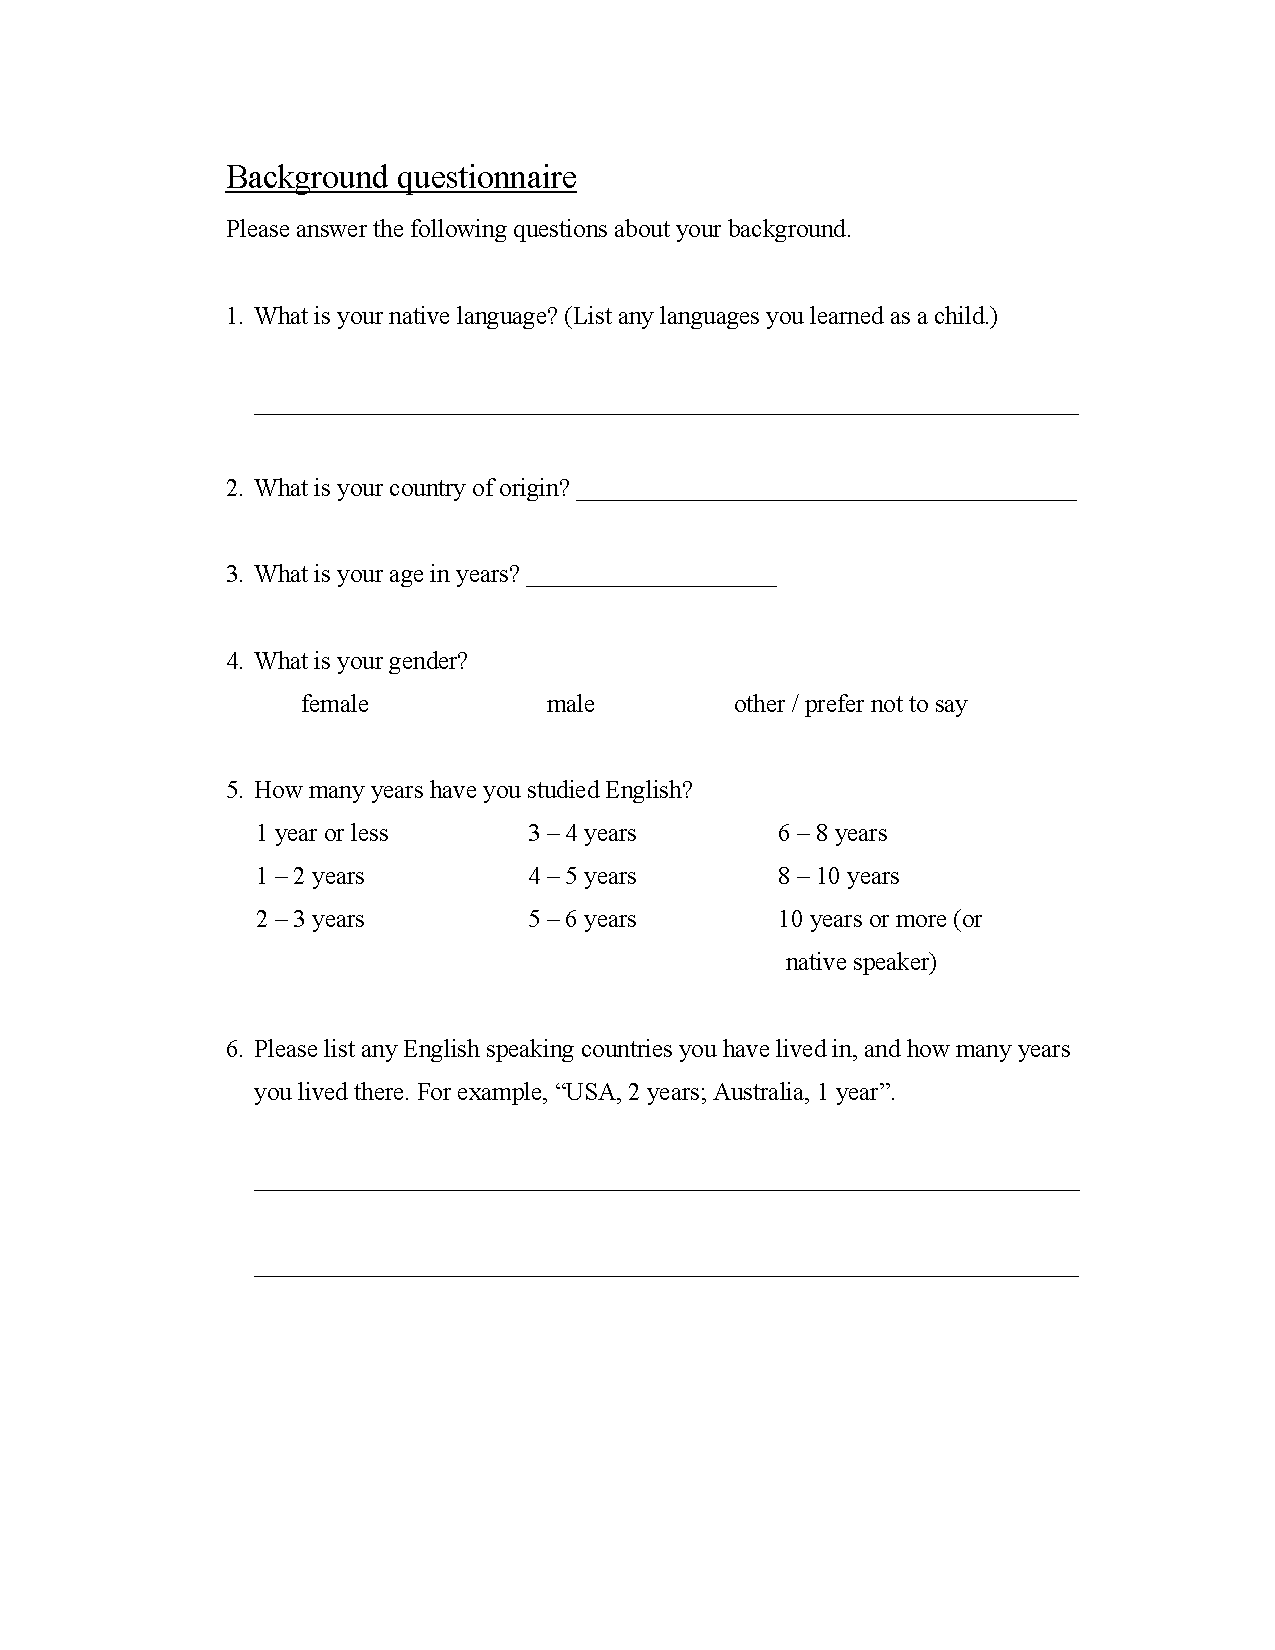
\includepdf[pages=-]{PDT_questionnaire.pdf}

\chapter{PDT Items}
\label{appendix:PDT_items}
The 30 picture description task (PDT) items are shown in this section. Each is displayed with its \textit{targeted} prompt. For all items, the \textit{untargeted} prompt is ``What is happening?'' Each item is marked as \textit{In}, \textit{Tr}, or \textit{Di} to denote it as either \textit{intransitive}, \textit{transitive}, or \textit{ditransitive}.

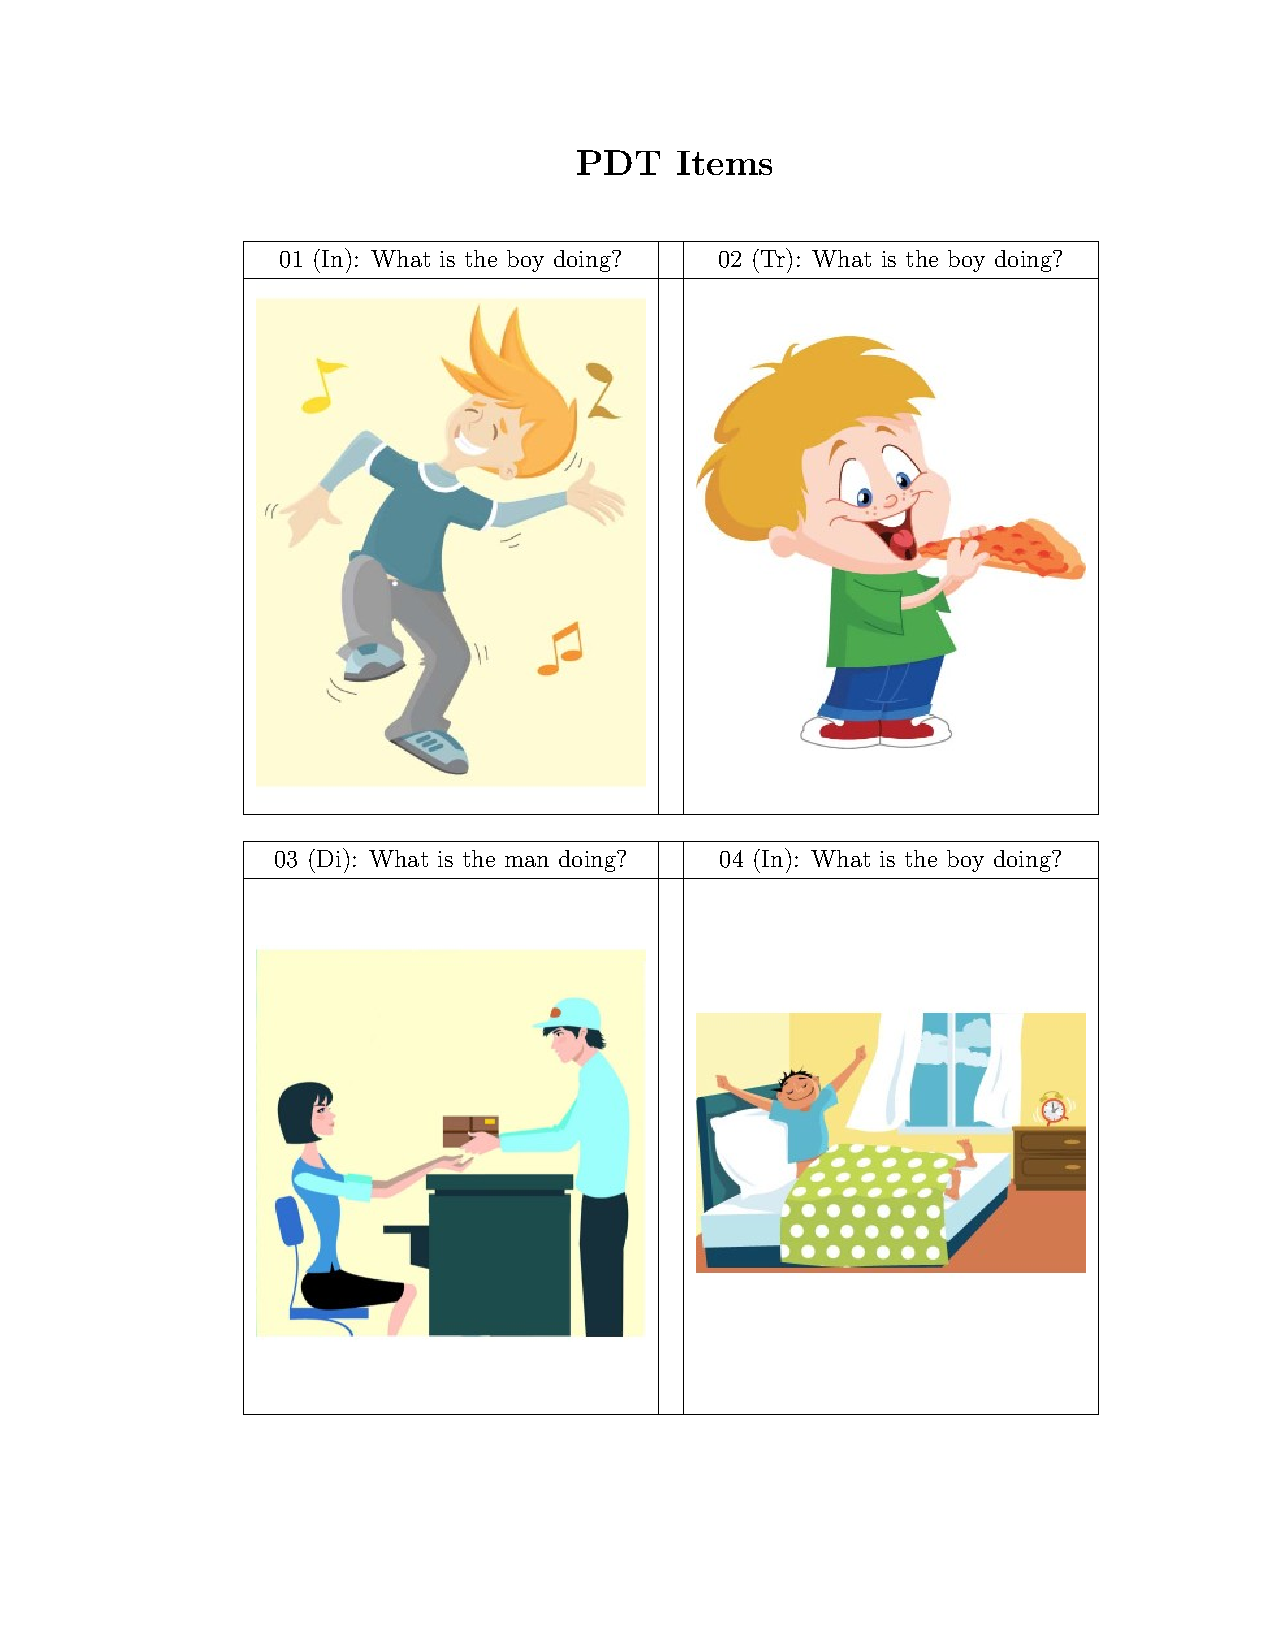
\includepdf[pages=-]{PDT_items_appendix_diss_format.pdf}

\chapter{Annotation Guide}
\label{appendix:annotation_guide}
The following pages consist of the annotation guide. This guide was produced through an iterative process of annotation and discussion between the researchers, annotators and outside linguists. This is the final version of the guidelines, which was used to produce the annotations included in the SAILS Corpus.

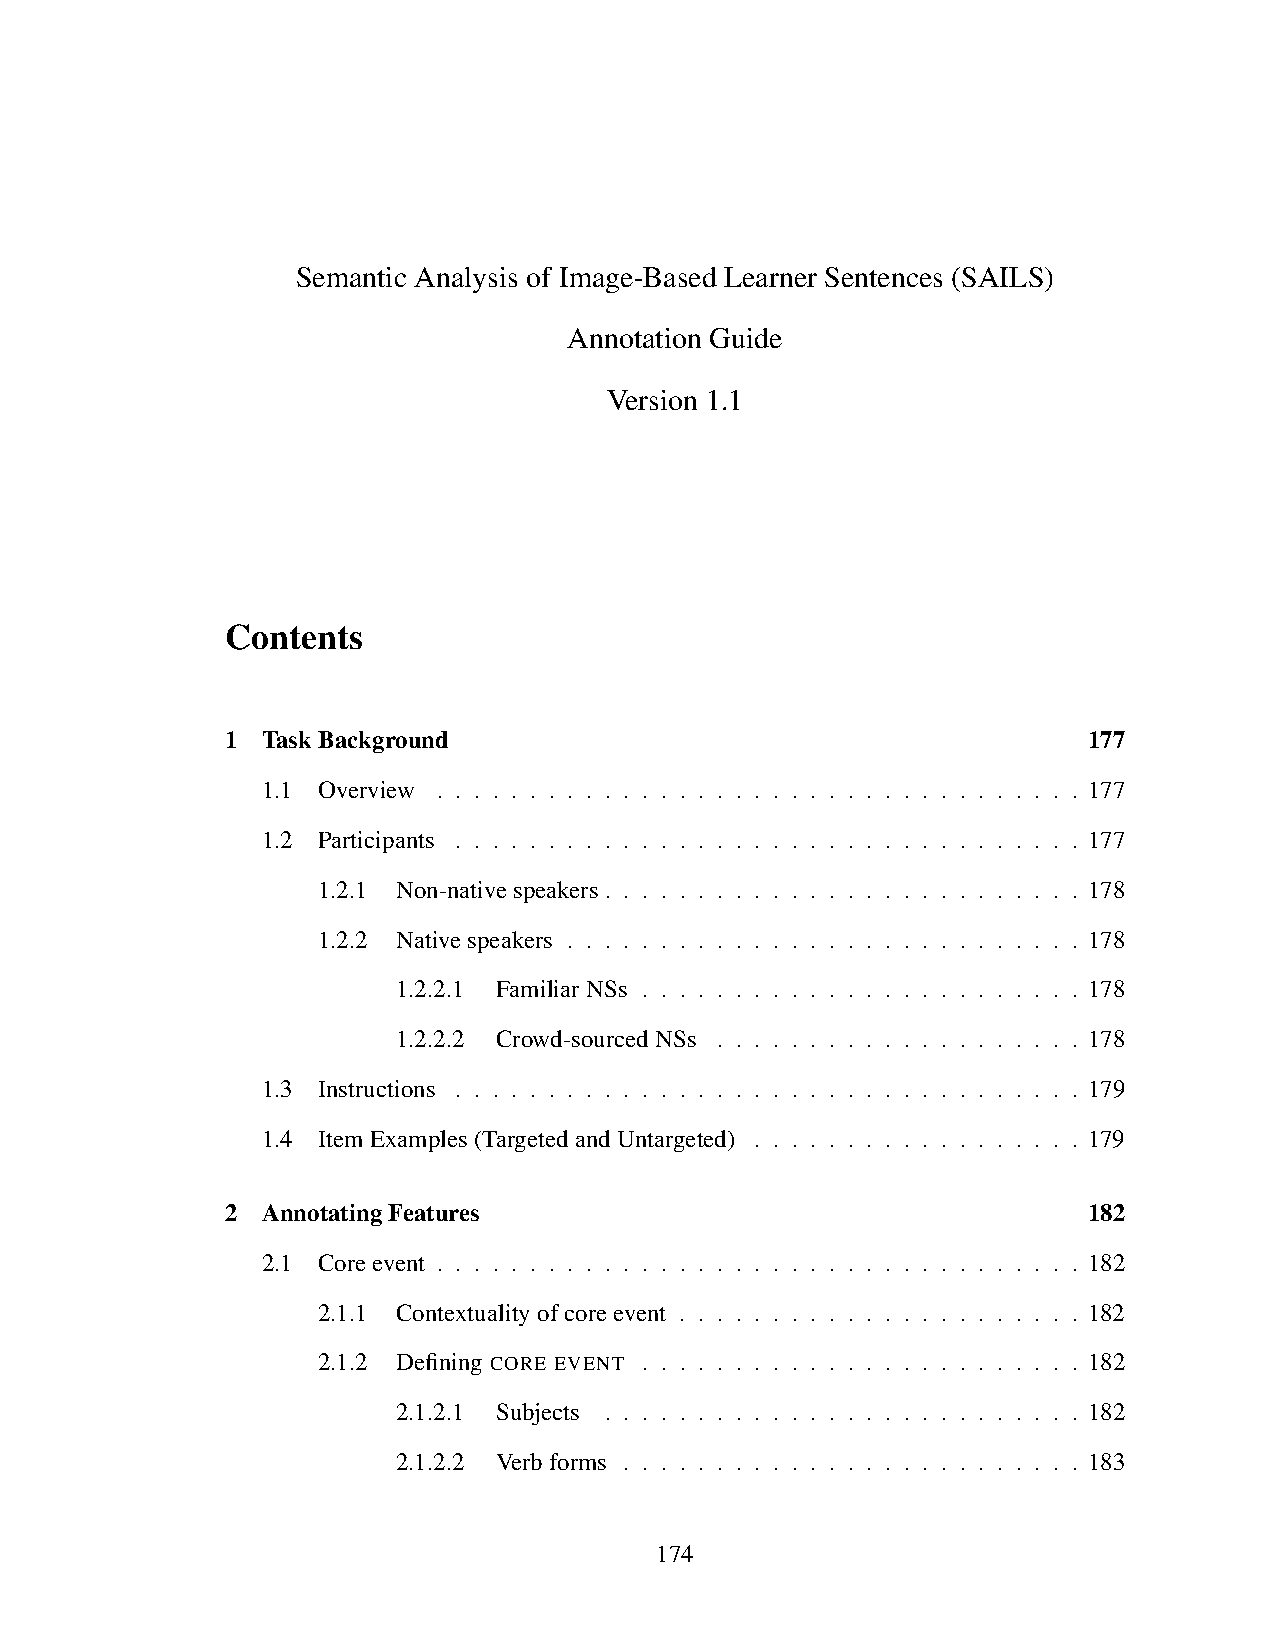
\includepdf[pages=-]{Annotation_Guide_Diss_Style.pdf}

\end{appendices}

%%%%%%%%%%%%%%%%
% References
%%%%%%%%%%%%%%%%
%\begin{singlespace}  % use single-line spacing for multi-line text within a single reference
%	\setlength\bibitemsep{\baselineskip}  %manually set separataion betwen items in bibliography to double space
%	\printbibliography[heading=bibintoc,title={References}]
%\end{singlespace}
%%\printbibliography[heading=bibintoc,title={References}]
%\addcontentsline{toc}{chapter}{References}  %add References section to Table of Contents
\bibliographystyle{acl_natbib}
\bibliography{levi.bib}
%%%%%%%%%%%%%%%%
% Vita 
% Only for PhD students
% Masters students remove this line
%%%%%%%%%%%%%%%%
%\chapter*{Vita}
\addtocontents{toc}{
 \unexpanded{\unexpanded{\renewcommand{\cftchapdotsep}{\cftnodots}}}%  
}
\addcontentsline{toc}{chapter}{Curriculum Vitae}


\includepdf[pages=-]{LK_CV.pdf}


\pagenumbering{gobble}

\end{document}
